% Supplementary text. First converted 2026-11-14 from explore/structure_vs_sequence/doc/structure_vs_sequence.tex
% (commit 25bae39 lineage) by scratch/make_supp.py, then edited here as source.
\section{Definitions: copies, arrangements, alignment columns and distances}\label{sec:compared}
\textbf{Structure} of a haplotype is the composition and order of the principal bundles (sequence blocks shared
across haplotypes) along its whole SMN window, as decomposed by PANGEA, the successor of PGR-TK~\cite{chin2023}.
The \emph{structural distance} between two windows is the score of \texttt{pangea cohort bundle dist} (0 =
same bundles in the same order). It reflects the large repeat units, hundreds of kilobases long, that carry the SMN copies, not the SMN genes themselves.

\textbf{Which haplotypes each comparison uses.} Of the \nHapsAll{} haplotypes, \nHapsRes{} are \emph{resolved} (the SMN region on one contig). Two different sets of the same size come from them: the \nHapsResSMNone{} resolved haplotypes that carry an SMN1 copy (\nHapsResNoSMNone{} carry none) and the \palHaps{} whose window has repeat units (\nHapsNoUnits{} have none). Structure is compared with SMN1 sequence (Mantel tests by lineage, the two trees, the bands) on \mlbHaps{} haplotypes: the \nHapsResSMNone{} resolved haplotypes with an SMN1 copy, and GRCh38 and CHM13; the SMN2-only Mantel test uses the \mTwoN{} haplotypes with an SMN2 copy; the all-copy Mantel test uses all \nHapsRes{} resolved haplotypes with the two references (\setAllCopy); the palindrome and arm results use the \palHaps{} with units; the ancestry tests use the \anHaps{} resolved haplotypes in the five continental groups, leaving out \setNoLab{} without a population label and \setAsl{} from ASL.

\textbf{Sequence} is the gene body of each counted SMN copy (SMN1, SMN2 and the hybrids h12 and h21, read from the
assemblies by the study's pipeline).

\textbf{Repeat units and their families (Table~\ref{tab:unitfam}; Fig.~\ref{fig:ruAlgo}).} A haplotype's \emph{window}
is the stretch of its contig that a PANGEA query of the GRCh38 stretch chr5:\wfGStart--\wfGEnd{} hits; every window
begins and ends in bundles that occur once in it (Fig.~\ref{fig:ruAlgo}a; Methods). PANGEA's \texttt{repeat-units}
(version 0.27.0, default settings) takes a window's bundle segments in order, each with a bundle id, a strand, a start and
an end, and works in six steps (Fig.~\ref{fig:ruAlgo}b,c):
\begin{enumerate}
\item \emph{Self-match.} Two segments with the same bundle id match: directly when on the same strand, inverted when on
opposite strands. This is a dot plot of the window against itself, in bundles.
\item \emph{Chains.} Matches are joined along diagonals (anti-diagonals for inverted matches). A step may skip up to
\ufMaxGap{} segments on both copies, or up to \ufMaxIndel{} on one copy (an indel), but not segments of the step's own
bundle, which would be another copy in a tandem array. A chain scores the bases of its matched segments, less, at each
step, a quarter of the difference between the bases skipped on the two copies.
\item \emph{Palindrome centers.} Where segments mirror each other outward from a point, on each side over at least the
minimum unit span and \ufMinMatch{} mirrored pairs, the point is a palindrome center; chains that cross it are cut there.
\item \emph{Tandem arrays.} A chain whose two copies overlap, with at least 90\% of its matches at one offset and at
least 2.5 units, is a tandem array; copies that fall in it are snapped to whole units.
\item \emph{Copies.} Chains are taken best first. A chain adds its two copies when they do not overlap, hold at least
\ufMinMatch{} matched segments and the shorter spans the minimum unit span (the median window span divided by 50, held
within 5--40~kb; \ufAutoKb{}~kb here). A copy that overlaps a known copy by half or more is that copy; otherwise it keeps
only the segments no earlier copy holds. Copies found by one chain are linked into one repeat.
\item \emph{Families.} A copy's \emph{bundle content} is the number of bases of each bundle id within its span, strand
ignored; a family's mean content is that number averaged over its members. Over all windows, copies are taken from the
longest. Each joins the family most similar to it by bp-weighted Jaccard similarity, the sum over bundle ids of the
smaller of the copy's and the family's bases divided by the sum of the larger, if that similarity is at least \ufJac{}
(a Jaccard distance of at most 1$-$\ufJac); otherwise it founds a family. The elements compared are thus bases, each labeled only by its bundle id: two copies share a base of bundle~$b$ wherever both hold one, whatever its exact sequence, and no k-mers or base-level alignment enter. Families are lettered by the bases they
cover, the most first.
\end{enumerate}
Over the \ufWindows{} windows this gives \ufOcc{} occurrences in \ufFams{} families (\ufInv{} inverted and \ufDir{}
direct relative to another occurrence; the shortest unit is \ufShortKb~kb, one of \ufBelowN{} \RU{\ufBelowFam} units
below the minimum span). Table~\ref{tab:unitfam} lists the \ufBig{} families with ten or more occurrences (the other
\ufSmallFams{} hold \ufSmallOcc). A family is defined by its bundle content, not by one fixed sequence; its \emph{core
bundles}, present in at least 90\% of its occurrences, are listed with the share of the family's bases they cover.

\begin{figure}[!htbp]\centering
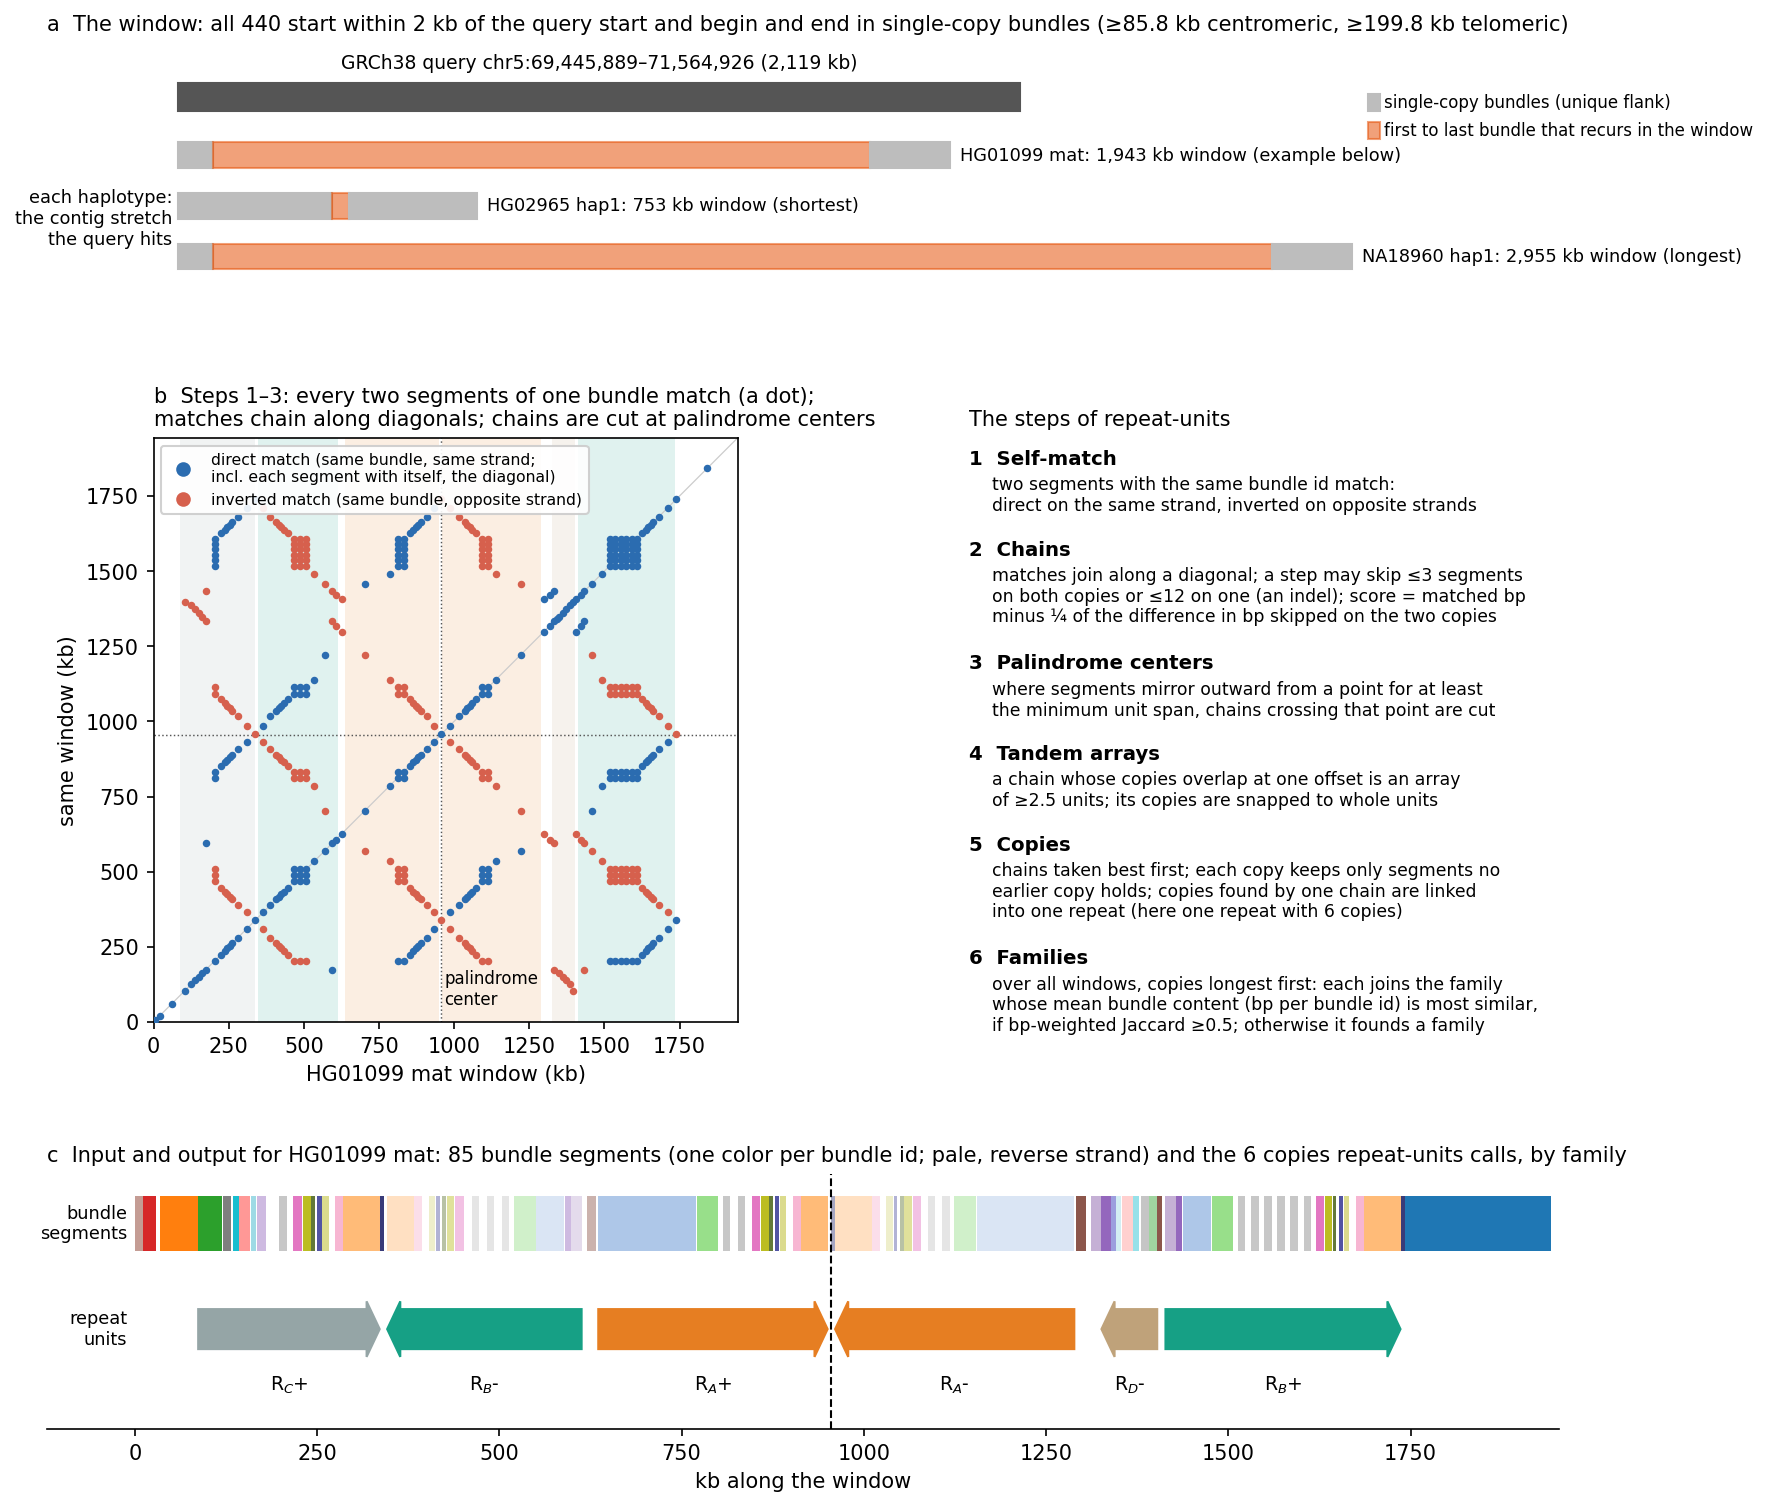
\includegraphics[width=\linewidth]{../figures/repeat_units_algo.png}
\caption{How a window is taken and how \texttt{repeat-units} turns it into repeat units. \textbf{a}, the window: the
stretch of each haplotype's contig hit by the GRCh38 query, drawn to scale for the example haplotype of b and c and for
the shortest and longest windows; gray, the single-copy bundles at each end; orange, from the first to the last bundle
that recurs in the window. \textbf{b}, the self-match of \ruaEx{} in bundles (step~1): one dot per pair of segments of
the same bundle, blue direct and red inverted; chains follow the lines of dots (step~2); the dashed lines mark the
palindrome center at which chains are cut (step~3); shading, the copies called, colored by family. Steps 1--6 are
summarized beside it. \textbf{c}, the input (\ruaSeg{} bundle segments, one color per bundle id, pale on the reverse
strand) and the output (\ruaUnits{} copies, by family and strand) for the same window. Drawn by
\texttt{scripts/39\_repeat\_units\_diagram.py}.}\label{fig:ruAlgo}
\end{figure}

\textbf{Units do not overlap in position, but they may be homologous to each other.} In a window no two units share more than the 55 bases ($k$) that neighboring bundle segments can share
(\ufPosOv{} pairs overlap by more; the ends of \ufKmerOv{} neighboring pairs touch by 1--55 bases; \ufOcc{} occurrences): \texttt{repeat-units} keeps the span of a copy found by a
better-scoring chain and gives a copy found later only the bundle segments that no known copy holds, and a final guard
splits any remaining overlap at its middle (steps 2 and 5 of the algorithm above). A family, however, is
defined by similarity of bundle content (bp-weighted Jaccard similarity at least \ufJac{} to the family's mean content; step~6), not by bundles of its own, so the
same bundles, and so the same sequence, recur in units of different families: the core bundles of \ufInA{} all lie
within \RU{A}'s (\RU{B} has exactly \RU{A}'s \ufABshared{} core bundles; see below), \ufPairsShare{} of the \ufPairs{} pairs of families in
Table~\ref{tab:unitfam} share at least one core bundle, and \ufBidsMulti{} of the \ufBids{} bundle ids found in units (an id counts when one of its segments lies within a unit's span)
appear in units of two or more families. Families \RU{A} and \RU{B} are the clearest case. Read in each unit's own orientation, both hold the same \ufABshared{} core
bundles in the same order and orientation (\ufABorder; in \ufAinOrd{} of \ufAn{} \RU{A} and \ufBinOrd{} of \ufBn{} \RU{B} units).
They differ in how much of two of them a unit holds and in what lies beside them: bundle~1 covers a median \ufAbOneA{} kb
in an \RU{A} unit against \ufAbOneB{} kb in an \RU{B} unit, the array bundle~15 \ufAbArrA{} against \ufAbArrB{} kb (the other
eight core bundles differ by at most \ufAbOtherMax{} kb), \ufBstartK{} \RU{B} units and no \RU{A} unit open with bundles 9+~8+,
and \ufAtenM{} \RU{A} units and no \RU{B} unit carry bundle 10$-$ before the core. In arm elements \RU{A} is mostly the core
(\feACore{} of its bases) and \RU{B} mostly Xi$'$ and Xi (\feBXi; Table~\ref{tab:unitfamel}): \RU{B} is the inverted copy of the core's
inner part, so the two families are one sequence seen from the two sides of the palindrome, cut at different places.

\textbf{Why \RU{A} and \RU{B} are two families although they share their core bundles.} The family rule (step~6
above) decides it, and it weighs bases, not bundle ids. \RU{A} was founded by the longest copy, \ufAfoundKb~kb. The
first \RU{B} copy, \ufBfoundKb~kb, scored \ufBfoundSim{} against \RU{A}'s mean content at that point, below the \ufJac{}
needed to join, and so founded a family of its own; each later copy joined the nearer of the two. The bases that set
them apart are those of two core bundles: the mean \RU{A} unit holds \ufMeanOneA~kb of bundle~1 against \ufMeanOneB~kb in
an \RU{B} unit, and \ufMeanArrA~kb of the array bundle~15 against \ufMeanArrB~kb. Every \RU{B} unit (\ufBcloser{} of
\ufBn) and \ufAcloser{} of the \ufAn{} \RU{A} units lie nearer their own family's final mean than the other's (median
similarity to their own mean \ufAownSim{} and \ufBownSim). The two families are nevertheless close: their final mean
contents have a similarity of \ufMeansSim, above the threshold, and \ufBgeThr{} of the \ufBn{} \RU{B} units would pass it
against \RU{A}'s final mean (median \ufBvsASim). \RU{A} and \RU{B} are thus two neighboring clusters of the same
sequence; where the line between them falls depends on the order in which the rule met the copies and on the
threshold, and taken in another order the two could have formed one family.

\textbf{How alike the families are in sequence.} The family rule compares bundle content. To compare sequence we took up
to \fsN{} units of each family with at least \fsMinOcc{} donor occurrences (\fsFams{} families, \fsUnits{} units, one per
haplotype) and, for every two units from different haplotypes (\fsPairs{} pairs), matched their shimmers (w24, k48,
r2) and took the Jaccard similarity of the two units' shimmer sets (shared over union; Fig.~\ref{fig:famshim}). Units
of one family are \fsJDiagLo--\fsJDiagHi{} alike, and \RU{A} and \RU{B} are the most alike pair of different families
(\fsJAB, against at most \fsJOtherMax{} for any other pair; \RU{B} with itself \fsJBB). Much of the spread within a
family is length: counted over the shorter unit's shimmers, units of one family are \fsODiagLo--\fsODiagHi{} alike
(\RU{B} \fsOBB), the shorter unit lying largely within the longer. Counted by direction, \fsCBA{} of an \RU{B} unit's
shimmers are found in an \RU{A} unit and \fsCAB{} the other way, so \RU{B} is largely a part of \RU{A}'s sequence;
\RU{D} lies largely within \RU{C} (\fsCDC{} against \fsCCD), and against \RU{A} or \RU{B} every median is at most
\fsDABMax. Shimmer positions are matched without their order, and the samples of \RU{F} and \RU{J} are small. Drawn by \texttt{43\_family\_shimmer.py}.

\begin{figure}[htbp]
\centering
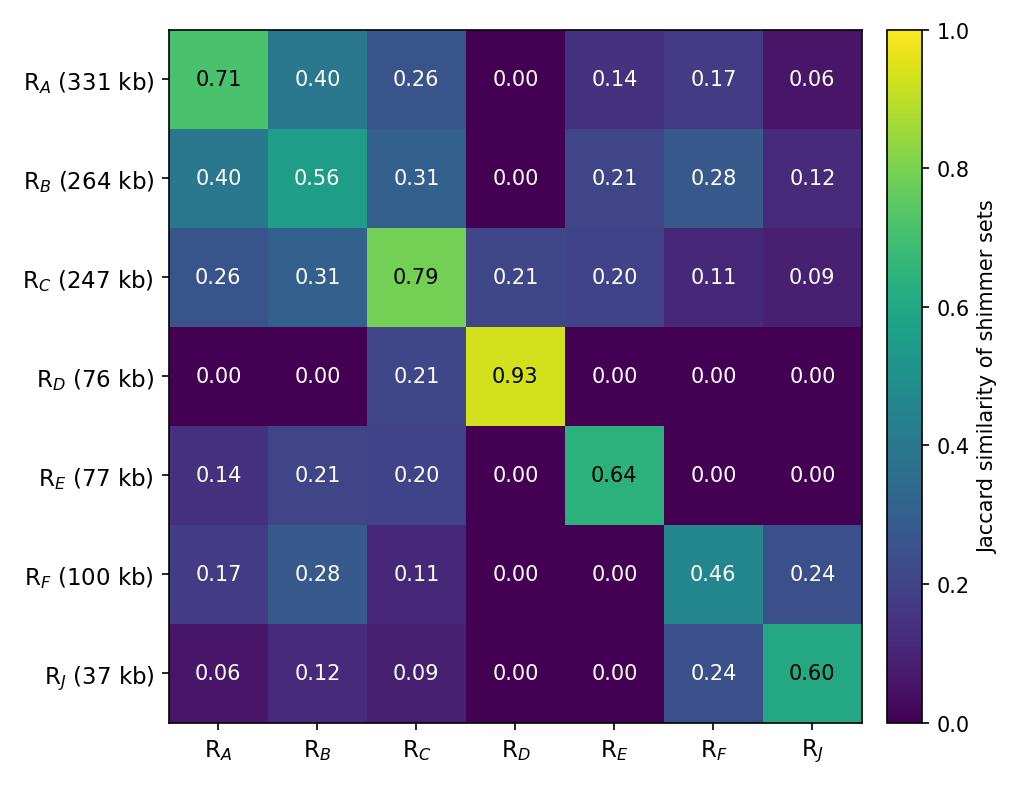
\includegraphics[width=0.62\linewidth]{../figures/family_shimmer.png}
\caption{Sequence similarity between repeat-unit families: Jaccard similarity of two units' shimmer sets (shared over
union), the median over pairs of units from different haplotypes (up to \fsN{} units per family, one per haplotype;
\fsPairs{} pairs). Row labels give the median length of the sampled units. Drawn by
\texttt{43\_family\_shimmer.py}.}
\label{fig:famshim}
\end{figure}

Which family a stretch of sequence is labeled with depends on
which chain claimed it first and where that chain stopped. The arms are compared by their elements, not their units
(Section~\ref{sec:palindrome}, Fig.~\ref{fig:palindrome}). The table is written by \texttt{33\_unit\_families.py} and \texttt{40\_numbers.py}.

\textbf{Why unit boundaries are not unique.} The region is built of nested repeats, in both orientations: the core and its inverted copy across the axis (the \RU{A}+\,\RU{A}$-$ pair), beyond the core an inverted copy of it, split by a tandem array into Xi$'$ and Xi, and Xi again in the core's orientation (Xd), with the spacer S at the center of each inverted pair (Section~\ref{sec:palindrome}, Table~\ref{tab:elements}). Read outward from the axis, the same bundles therefore recur several times, at different distances and in both orientations, and a repeat finder has to choose which copies to pair and where each copy ends. PANGEA's \texttt{repeat-units} pairs them from the best-scoring chain outward and gives later chains only what is left (above), so homologous sequence is labeled \RU{A} on one arm and \RU{B} on another, and an \RU{A} unit stops before the core's end or runs past it over E according to what the other arm holds there: both \RU{A} units run past the core on \auCZeroBoth{} of the \auCZeroHaps{} C0 haplotypes and neither does on \auCOTZeroNeither{} of the \auCOTZeroN{} C1|T0 haplotypes (Section~\ref{m:arms}). Other pairings of the same sequence are possible, for example the inverted core copy (Xi$'$ and Xi) with the inner part of the core on its own arm rather than with its counterpart on the other arm, so the units are one consistent reading of the region, not the only one.

\textbf{Five windows as bundles, units and elements (Fig.~\ref{fig:pgraph}).} PANGEA first builds a graph of
shimmer pairs shared by the sequences and then reads principal bundles off it. A shimmer is a sparse minimizer (a $k$-mer chosen as the smallest
in its window, with only a fraction of them kept), and a shimmer pair is two consecutive shimmers along a sequence; in the graph each vertex is a shimmer pair and
an edge joins two pairs that follow each other in some sequence, so that sequence shared by several haplotypes runs as one path. Fig.~\ref{fig:pgraph}
shows what the study's decomposition (\texttt{results/decomp/smn.bed}, the settings of Table~\ref{tab:decomp}) makes of five windows (HG03816 pat, HG01099 mat, GRCh38, CHM13 and \grBand, a
``1-~1+'' haplotype of the B1\,+\,B2 band): \grSegs{} bundle segments from \grBundles{} bundles, and under them the
repeat units of Table~\ref{tab:unitfam} and the arm elements of Section~\ref{sec:palindrome}. Bundles, units and elements all come from the study's own decomposition, so the bundle ids are those of Table~\ref{tab:unitfam}.

HG03816 pat and HG01099 mat (the top two windows of Fig.~\ref{fig:pgraph}) carry the same arm elements in the same order and, at the study's bundle scale, the same repeat units. With the finer bundles of Section~\ref{sec:fine} PANGEA cut one of them into a short \RUf{A} unit and \RUf{B} units and gave the other one long \RUf{A} unit (Section~\ref{sec:fine}).

\begin{figure}[htbp]\centering
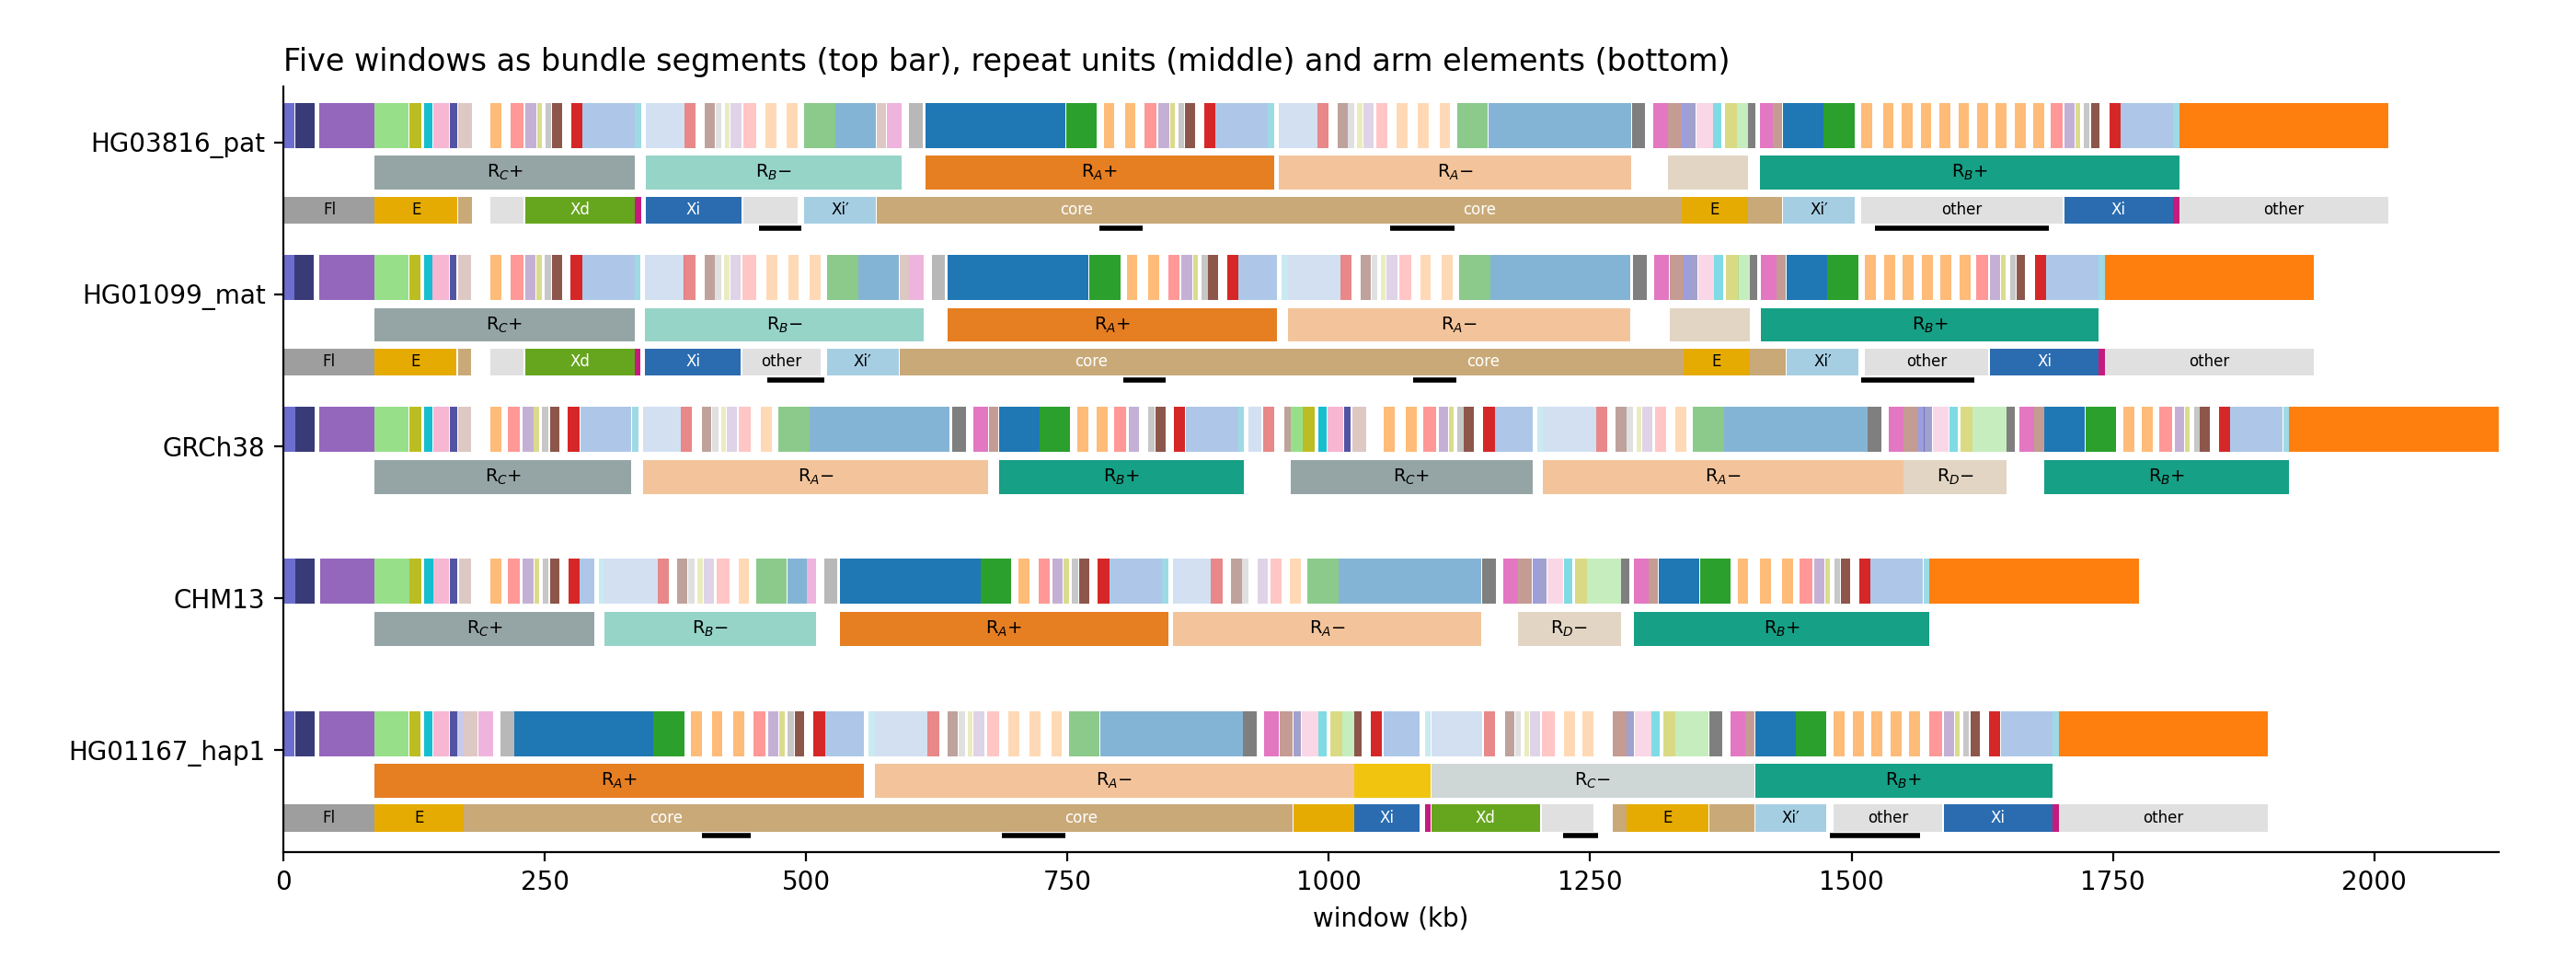
\includegraphics[width=\linewidth]{../figures/window_bundles.png}
\caption{Five SMN windows in the study's bundle decomposition (\texttt{pangea cohort bundle decomp}, $w=48$, $k=55$, $r=4$; all settings in Table~\ref{tab:decomp}): for each
window, bundle segments (top bar; one color per bundle id; pale, reverse
direction), the study's repeat units (middle bar, family colors as in Fig.~\ref{fig:allhaps}) and, for the three windows
with an \RU{A}+ \RU{A}$-$ pair, the arm elements of step 28b (bottom bar, colors as in Fig.~\ref{fig:palindrome}; black lines,
the $\sim$20~kb tandem arrays).}\label{fig:pgraph}
\end{figure}


\begin{table}[htbp]\footnotesize\centering
\caption{Repeat-unit families with ten or more occurrences, from PANGEA's \texttt{repeat-units} output
(\texttt{results/decomp/smn.repeat\_units.tsv}) and the bundle decomposition. Occ.: unit occurrences; windows: windows
(haplotypes and the two references) carrying the family; span of an occurrence; bundles: median number of bundle
segments in an occurrence; strand of the occurrence (+/$-$); its relation to the other copy (inverted/direct); core
bundles: the bundle ids present in at least 90\% of the family's occurrences, with the share of the family's bases
they cover (core bp). Bundle ids are those of \texttt{results/decomp/smn.bed}.}\label{tab:unitfam}
\begin{tabular}{@{}lrrlrrrp{4.1cm}r@{}}\toprule
Family & Occ. & Windows & Span, kb (range) & Bundles & +/$-$ & Inv./dir. & Core bundles (number: ids) & Core bp\\\midrule
\tabUnitFam
\bottomrule\end{tabular}
\end{table}

\begin{table}[htbp]\footnotesize\centering
\caption{What each repeat-unit family is made of, in the arm elements of Section~\ref{sec:palindrome}. For every unit
occurrence on the \elHaps{} haplotypes with the head-to-head \RU{A} pair, the share of its bases in each element (core: within the
arm's core; core end; Xi, both parts, Xi$'$ and Xi; S; Xd; E; flank; other: bases in none of these elements), averaged per family, so each row adds to 1; last column, the commonest combination of elements
with a share of at least 0.1, and how many occurrences have it. Families with ten or more such occurrences. Written by
\texttt{40\_numbers.py} from \texttt{results/sv/unit\_family\_elements.tsv} (step 28e).}\label{tab:unitfamel}
\begin{tabular}{@{}lrrrrrrrrrrl@{}}\toprule
Family & Occ. & Hap. & Core & Core end & Xi & S & Xd & E & Flank & Other & Commonest (occ.)\\\midrule
\tabUnitFamEl
\bottomrule\end{tabular}
\end{table}

\textbf{Copy classes.} The study's pipeline names each copy by two paralog-specific bases read in the copy's own
sequence: c.840 in exon~7 and c.*239 in exon~8. An \emph{SMN1} copy carries the SMN1 base at both, an \emph{SMN2}
copy the SMN2 base at both. A \emph{hybrid} carries one of each: \emph{h12} has SMN1's exon~7 and SMN2's exon~8,
\emph{h21} the reverse. A $\Delta$7--8 copy lacks exons 7 and 8. A counted copy lies away from contig ends and gaps and is either whole (all nine exons:
1, 2a, 2b and 3--8) or a $\Delta$7--8 copy (exons 1--6); a \emph{truncated} piece is cut short by a contig end or gap and a \emph{fragment} misses
part of the gene elsewhere, and neither is counted as a copy.

\textbf{Arrangement type.} The \emph{arrangement} of a haplotype is the string of its SMN copies in order along its
window, from the centromeric end to the telomeric end (GRCh38 coordinate order), each written as a class code followed
by its strand. The codes are \texttt{1} (SMN1), \texttt{2} (SMN2), \texttt{h12} and \texttt{h21} (the hybrids),
\texttt{d2} (a $\Delta$7--8 copy of SMN2 type), \texttt{t} (a truncated piece) and \texttt{f} (a fragment). The
strand is \texttt{+} when the copy runs on the forward strand of the window held in GRCh38 orientation (the
orientation read from the window's own sequence), as SMN1 does in GRCh38, and \texttt{-} when it runs on the other.
So ``2-~1+'' is a reversed SMN2 copy on the centromeric side of a forward SMN1 copy, two copies in head-to-head
inverted orientation; ``1+'' is a single forward SMN1 copy; and ``1-~h12+~1+'' is three copies. GRCh38 itself reads
``2+~1+'' and CHM13 ``2-~1+''. ``1-~h21$\pm$'' stands for ``1-~h21+'' and ``1-~h21-'' together.

An
\emph{arrangement type} is one distinct string; haplotypes with the same string share the type. Over the \arrHaps{}
resolved haplotypes (the region on one contig, spanned end to end) there are \arrTypes{} types, \arrOnce{} of them
seen on one haplotype only; the commonest, ``2-~1+'', is on \arrTopN. Uncounted pieces are kept in the strings, which
adds \arrUncTypes{} types (``f-~1-'' and ``t-~2-~1+''), and they are built by the study's pipeline
(\texttt{scripts/05\_haplotype\_calls.py}). \emph{Centromeric} and \emph{telomeric} for a single copy are defined in
Section~\ref{sec:posstrand}.

\textbf{Alignment columns.} The copies are compared through one multiple sequence alignment made by MAFFT: a table
with one row per copy and one \emph{column} per aligned position. A column holds, for each copy, the base it carries
at that position, or a gap (`-') where it has none; MAFFT places the gaps so that the bases in one column are taken
to be the same position of the gene in every copy. The alignment has \nAlnRows{} rows (each copy cut with 2~kb of flank on each
side, all on the SMN1 strand) and \nAlnCols{} columns, more than any one copy's length because an insertion in any
copy adds columns where all other copies have gaps. The \emph{gene-body columns} are those between the flanks,
measured on the GRCh38 SMN1 copy: the \nRefBody{} columns where that copy has a base (its \nRefLen{} bases, less
2{,}000 at each end), plus the \nInsCols{} columns inside that stretch where it has a gap and some other copy has a
base (insertions in other copies, such as longer poly-T runs). That makes \nGeneCols{} gene-body columns. A column is
therefore a position of the alignment, not a base of GRCh38; a position in this document given as chr5:\ldots{} is
the GRCh38 base in that column (for an insertion column, the GRCh38 base just before it).

The \emph{copy distance} is the share of differing bases between two copies (p-distance), counted over the
gene-body columns where both copies carry a base (A, C, G or T); columns where either copy has a gap or an N are
skipped, so a pair is compared over somewhat fewer than \nGeneCols{} columns. \nVarCols{} of the gene-body columns
vary among the copies. The \emph{sequence distance} between two haplotypes is the mean,
taken both ways, of each copy's distance to its nearest copy on the other haplotype. It is computed over all copies,
over SMN1 copies only and over SMN2 copies only; the last two compare lineages without mixing in which genes a
haplotype carries.

\textbf{Copies used.} Of the \nCounted{} counted copies, \nAligned{} were aligned; the \nJoined{} copy the pipeline joined from two
pieces of one contig (an SMN2 copy of HG00597 mat) was not. The \nDelLeftOut{} $\Delta$7--8 copies were then left
out because the aligner misplaced their 6.3-kb deletion, leaving \nCopies{}: \nSMNone{} SMN1, \nSMNtwo{} SMN2,
\nHtwelve{} h12 and \nHtwentyone{} h21. By continental group (1000 Genomes superpopulation of the donor), they are
\spAFR{} AFR, \spEAS{} EAS, \spAMR{} AMR, \spSAS{} SAS and \spEUR{} EUR, \spOther{} from donors with no group in this
scheme (one ASL donor, and HG002 and HG005, which carry no population label in the study's table) and \spNone{} from
GRCh38 and CHM13.

\section{Pipeline steps and software}
Table~\ref{tab:tools} lists each step with the program that does it, its version and what it reads
and writes. The diagrams are drawn by Matplotlib from the distance matrices; PANGEA, MAFFT and IQ-TREE make the
inputs.

\begin{table}[!h]\small\centering
\caption{The steps, in order. \texttt{scripts/run\_all.sh} runs them in order from the project's root.}
\label{tab:tools}
\begin{tabular}{@{}>{\raggedright}p{2.6cm}>{\raggedright}p{3.4cm}>{\raggedright\arraybackslash}p{9.6cm}@{}}
\toprule
Step & Tool (version) & What it does here \\
\midrule
Bundle decomposition & PANGEA \verPangea{}, \texttt{cohort bundle decomp}, \texttt{repeat-units}~\cite{chin2023} & \texttt{00\_windows\_decomp.py}: extracts the \wfN{} windows, decomposes them together (settings in Table~\ref{tab:decomp}) and calls the repeat units; writes \texttt{results/decomp/}. \\
Structural distance & PANGEA \verPangea{}, \texttt{cohort bundle dist}~\cite{chin2023} & Reads the study's bundle
decomposition of every window (\texttt{results/decomp/smn.bed}) and scores each pair of windows by its top bundles;
writes \texttt{results/sv/smn\_struct.dist}. Step 01b does the same on the finer decomposition (\texttt{results/bundles/smn.bed}; Section~\ref{sec:fine}). \\
Copy alignment & MAFFT \verMafft{}, FFT-NS-2~\cite{katoh2013} & \texttt{02\_copy\_alignment.sh}: aligns the \nAligned{} copies
(gene body with flanks, all on the SMN1 strand) progressively; writes \texttt{results/sv/copies.aln.fa}. Its engine,
\texttt{disttbfast}, takes most of the run time. \\
ML tree & IQ-TREE \verIqtree{}, \iqModel, \iqBoot{} ultrafast bootstraps~\cite{minh2020,hoang2018} & \texttt{04a\_ml\_tree.sh}: the
\iqSeqs{} rows (the copies without the $\Delta$7--8 copies, plus four apes) over the \iqCols{} gene-body columns, rooted
on the orangutan copy (\iqIdent{} identical sequences set aside and re-attached); \texttt{29\_ml\_tree\_clades.py} reports
its clades; Fig.~\ref{fig:mltree}. \\
Distances, tests, trees, plots & Python: NumPy \verNumpy{}~\cite{harris2020}, pandas \verPandas{}, SciPy \verScipy{}~\cite{virtanen2020},
Matplotlib \verMpl{}~\cite{matplotlib} & \texttt{07\_compare.py}: p-distances over the gene-body columns; Mantel tests
(Spearman, \nPerm{} permutations)~\cite{mantel1967}; the UPGMA structure tree with optimal leaf order; cophenetic correlation;
nearest-neighbor agreement; the three figures. \\
Ape bases at the history sites & agc-rs, Python (as above) & \texttt{13c\_ape\_site\_reads.py}: each ape's base at every S and A/B site, read from its raw primary-assembly sequence by local alignment of the GRCh38 context (\rdAcc{} of \rdN{} reads kept); step~16 uses these bases. \texttt{36\_window\_flanks.py}: how each SMN window was taken and its single-copy ends. \\
Spacer sequence & Python: edlib \verEdlib{}& \texttt{28c\_spacer\_sequence.py}: puts each S occurrence in the reference orientation by \sK-mer containment and aligns it end to end to the others (global edit distance), which gives the Sa and St variants of Section~\ref{sec:palindrome}. \\
This document's numbers & Python (as above) & \texttt{40\_numbers.py}: every number below as a macro, with checks;
recomputes the copy tree to place the \cpe{} copies. \\
\bottomrule
\end{tabular}
\end{table}

\section{Large-scale structure against SMN sequence}\label{sec:structseq}
\subsection{Haplotypes with similar structure carry similar SMN copies (Fig.~\ref{fig:scatter})}\label{sec:cophen}
Each dot is one pair of haplotypes. Pairs of the same arrangement type (Section~\ref{sec:compared}) are drawn in orange, pairs of different types in gray. Same-type pairs sit low and left:
their median structural distance is \structSame{} against \structDiff{} for different-type pairs, and their median
sequence distance (all copies) \seqSame{} against \seqDiff{} differences per kb. The horizontal bands come from
the sequence distance being a small whole number of differences divided by the gene length.
The rank correlation, tested by the Mantel test (the haplotype labels of one distance matrix shuffled, \nPerm{} times),
is \mantelAll{} for all copies and \mOneR{} for SMN1 copies; each $p$ is \mantelP{}, the smallest \nPerm{} shuffles
can give, also when shuffling only within African-ancestry and other haplotypes, or within each of five continental groups (\textbf{Shuffles within five groups}, below). Within African-ancestry haplotypes the
SMN1 correlation is \mOneAFRlower{} (\mOneAFRR{}, \mOneAFRN{} haplotypes) than within the rest (\mOneNonAFRR{},
\mOneNonAFRN{} haplotypes).

\begin{figure}[h]\centering
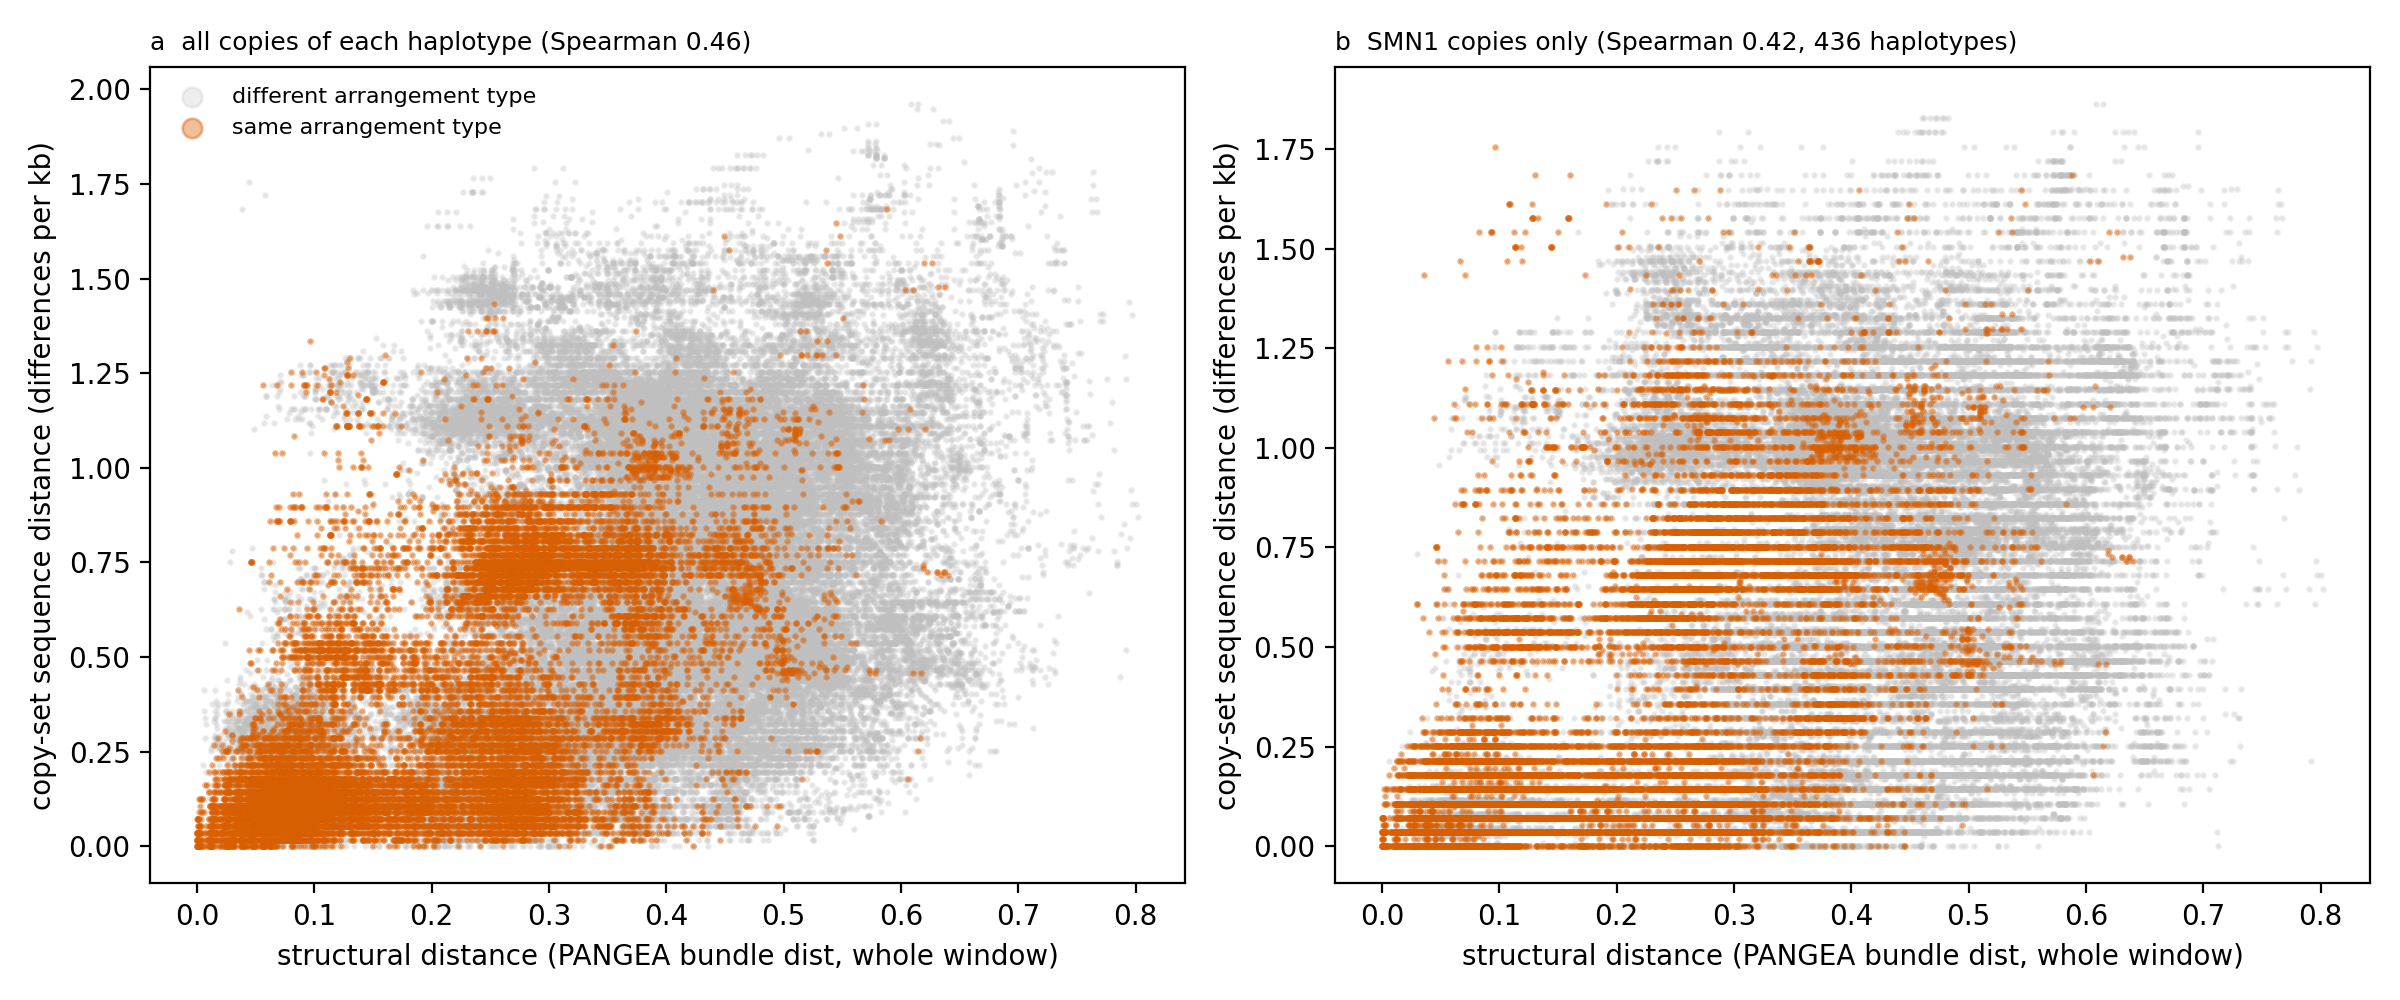
\includegraphics[width=\linewidth]{../figures/hap_scatter.png}
\caption{Each pair of haplotypes by structural distance (x; PANGEA bundle distance over the whole window) and
sequence distance of their SMN copies (y; differences per kb). \textbf{a}, all copies; \textbf{b}, SMN1 copies only.
Orange, the two haplotypes have the same arrangement type. Drawn by \texttt{07\_compare.py}.}
\label{fig:scatter}
\end{figure}

\paragraph{Within one arrangement type (Fig.~\ref{fig:scattype}).} Drawn one type at a time, the same-type pairs of
the \stTypes{} types carried by ten or more haplotypes (\stTypeHaps{} haplotypes) do not form one cloud each: most
types split into a few clusters of pairs, low on both axes or higher on both. Across those clusters, structure and
sequence still go together inside a type: the within-type rank correlation is \stRlo{} to \stRhi{} in \stSigTypes{}
types (\stRbig{} for ``2-~1+''; Mantel test, haplotype labels shuffled within the type, each $p$ at the floor
\mantelP{}). The exception is \stNsType{} (\stNsN{} haplotypes, \stNsR{}, $p = \stNsP{}$). By eye, within a single
cluster of pairs the correlation is weak, so much of the within-type correlation comes from the clusters sitting apart;
this was not tested.

Types differ in how varied they are (Fig.~\ref{fig:scattype}h). The single-copy types are the most varied in
sequence: median distance \stQOne{} differences per kb for ``1-'' and \stQPlus{} for ``1+'', against \stQBig{} for
``2-~1+'' and \stQMix{} for ``1-~2+''. ``1-'' is also the most varied in structure (median \stSOne{}, against
\stSMix{} for ``1-~2+'' and \stSBig{} for ``2-~1+'').

\paragraph{Structural distance follows window length.} PANGEA's bundle distance scores the whole window, so two
haplotypes whose windows differ in length differ in structure even with the same SMN arrangement. Over same-type pairs
the structural distance has a rank correlation of \stLenSame{} with the difference in window length
(Fig.~\ref{fig:scattype}i; \stLenAll{} over all pairs), while the sequence distance has \stLenSeqAll{} over all pairs.
The single-copy windows are also the shortest (median \stLOne{} kb for ``1-'', \stLPlus{} kb for ``1+'', against
\stLBig{} kb for ``2-~1+''). Holding the length difference fixed (partial rank correlation), structure and sequence still
go together in the common two-copy types (\stPBig{} for ``2-~1+'', \stPInv{} for ``1-~1+'', \stPFlip{} for ``2-~1-''),
less in ``1+'' (\stPPlus{}), and hardly at all in ``1-'' (\stPOne{}) and ``1-~2+'' (\stPMix{}). So in those two types
the structural spread is mostly a matter of length, not of what the copies carry. Window length here is the length of
the copy-bearing window; every haplotype tested has one.

\begin{figure}[p]\centering
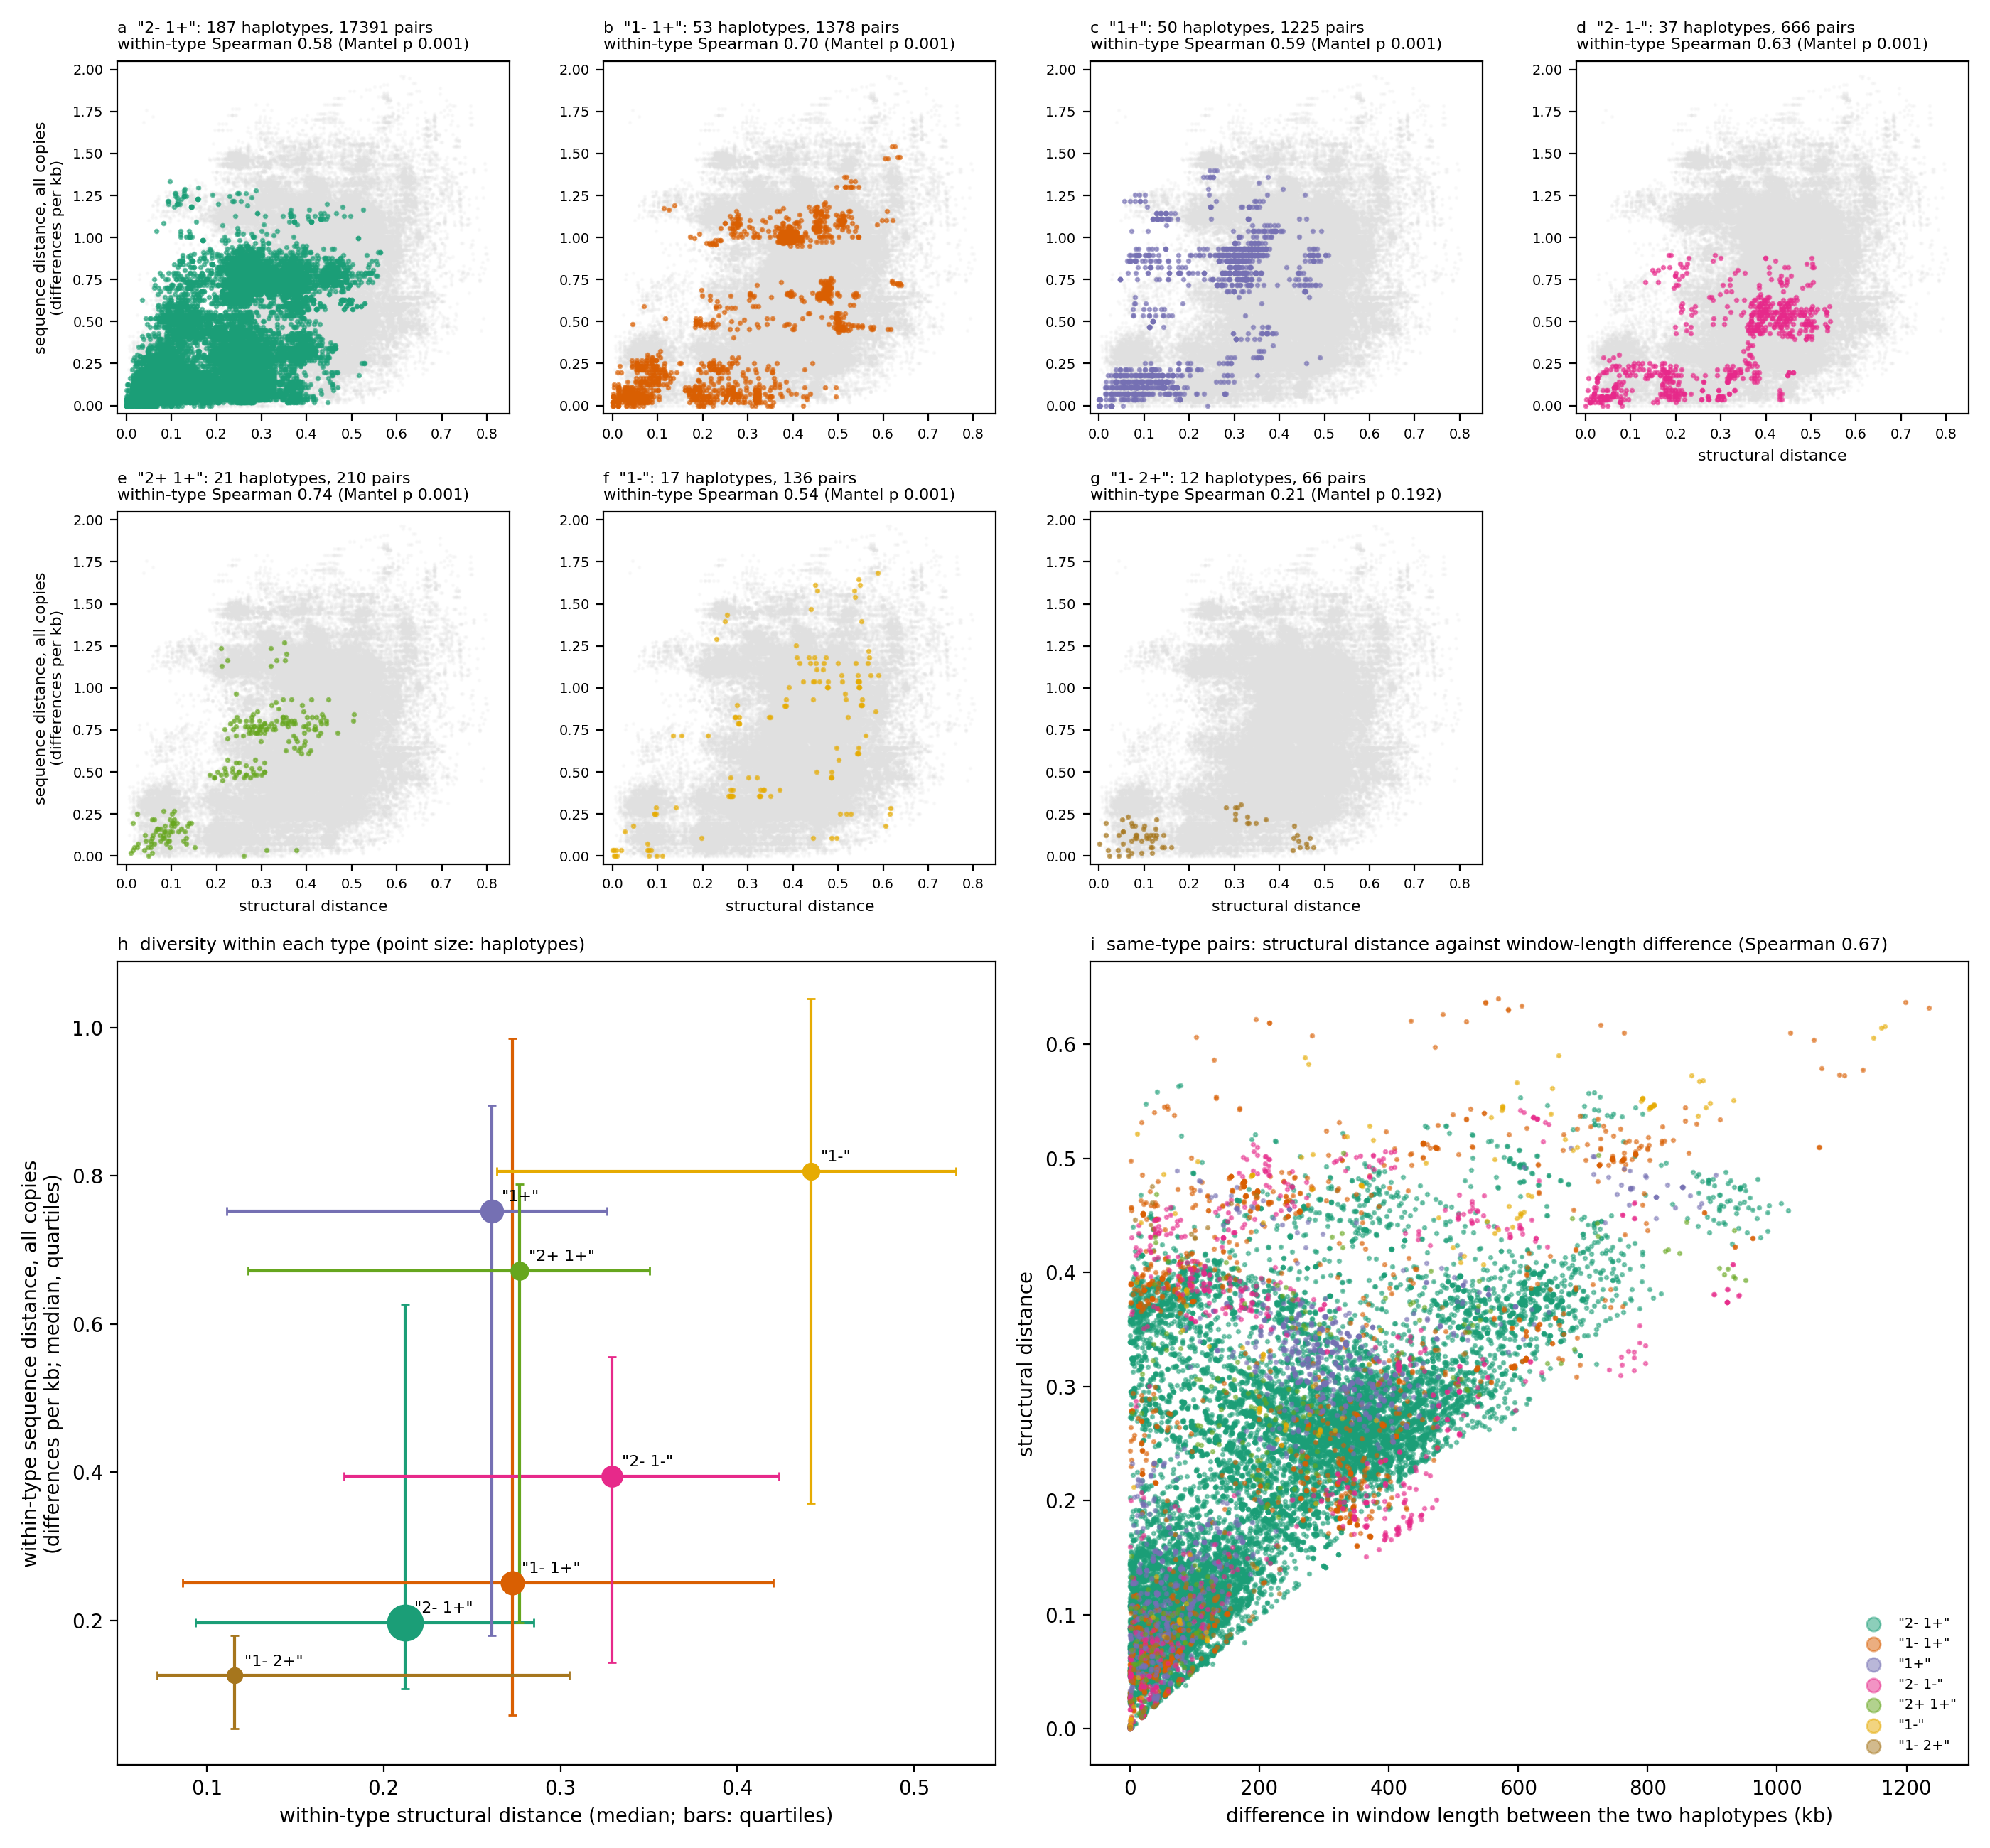
\includegraphics[width=\linewidth]{../figures/hap_scatter_bytype.png}
\caption{Fig.~\ref{fig:scatter}a taken apart by arrangement type. \textbf{a--g}, pairs of the same type (colored)
over all other pairs (gray), one panel per type with ten or more haplotypes, with the within-type rank correlation and
its Mantel $p$. \textbf{h}, within-type median structural and sequence distance; bars, quartiles; point size, number of
haplotypes. \textbf{i}, same-type pairs: structural distance against the difference in window length. Drawn by
\texttt{24\_scatter\_by\_type.py}.}
\label{fig:scattype}
\end{figure}

\paragraph{The two trees agree only loosely.} The structure tree of the \nTangle{} haplotypes that carry an SMN1 copy
(the \nHapsResSMNone{} resolved donor haplotypes with one, plus GRCh38 and CHM13; UPGMA on structural distance) and the
gene-body maximum-likelihood tree (main text, Fig.~\ref{fig:mltree}) agree only loosely: the cophenetic correlation, the
correlation between the heights at which two haplotypes join in the structure tree and the distance between their SMN1
copies along the branches of the maximum-likelihood tree (for a haplotype with two SMN1 copies, each copy's nearest copy
in the other haplotype, averaged both ways), is \cophenetic{}. These tree distances follow the p-distances closely
(Spearman \cophMlVsP). Where the trees do agree is taken up below, by SMN1 lineage make-up (Section~\ref{sec:lintrees}) and
as bands (Section~\ref{sec:bands}).

\subsection{A copy's nearest sequence neighbor tends to share its arrangement type (Table~\ref{tab:nn})}
Each of the \nCopies{} copies is given labels of its context in the haplotype: its copy order, its rank among all SMN copies of the
window, SMN2 and hybrids included (centromeric, middle, telomeric or the only one; defined in
Section~\ref{sec:posstrand}), its strand on GRCh38, the form of the NAIP gene at its 3$'$ side, the downstream
environment, the arrangement type of its haplotype and the donor's continental group (copies on unresolved haplotypes
are not assessed). The main text's Fig.~\ref{fig:mltree} draws the class, haplogroup, arm (cenSMN, telSMN or no \RU{A} pair), arrangement type and continental group
of each copy along the maximum-likelihood tree.

For each copy, the nearest copy by sequence on another haplotype was found
within SMN1 and within SMN2 separately, and the share of copies whose neighbor has the same label was compared with
the share expected by chance, from \nPerm{} shuffles of the label (Table~\ref{tab:nn}). For SMN1, neighbors share the
arrangement type \agArrOne{} of the time against \agArrNullOne{} by chance within ancestry groups, copy order
\agPosOne{} against \agPosNullOne{}, and strand \agStrOne{} against \agStrNullOne{}. For SMN2 the same figures are
\agArrTwo{} against \agArrNullTwo{}, \agPosTwo{} against \agPosNullTwo{}, and \agStrTwo{} against \agStrNullTwo{}.
Of the labels tested within ancestry groups, the arrangement type rises most above chance in both genes; ancestry itself, which can only be shuffled among all copies, rises by about as much in SMN1 (Table~\ref{tab:nn}). Nearly every SMN2 copy sits in an SMN2-type
environment, so that label adds little there (\agEnvTwo{} against \agEnvNullTwo{}, $p=\agEnvPTwo$).

\begin{table}[h]\small\centering
\caption{Nearest sequence neighbor on another haplotype: share with the same label. $n$, copies with the label
assessed; obs., observed share; chance, mean over \nPerm{} shuffles of the label among all copies, and among
copies of the same ancestry group (African ancestry or not); $p$ for the latter. Ancestry itself is tested only
against all-copy shuffles. Written by \texttt{40\_numbers.py} from \texttt{results/sv/copy\_neighbor\_agreement.tsv}.}
\label{tab:nn}
\setlength{\tabcolsep}{3.5pt}
\begin{tabular}{@{}>{\raggedright}p{4.3cm}rrrrr rrrrr@{}}
\toprule
& \multicolumn{5}{c}{SMN1 copies} & \multicolumn{5}{c}{SMN2 copies}\\
\cmidrule(lr){2-6}\cmidrule(l){7-11}
Label & $n$ & obs. & chance & \shortstack{chance\\ in group} & \shortstack{$p$\\ in group} & $n$ & obs. & chance & \shortstack{chance\\ in group} & \shortstack{$p$\\ in group} \\
\midrule
\tabNeighbor
\bottomrule
\end{tabular}
\end{table}


\subsection{Haplotypes with two B copies cluster in both trees; those with one B have like neighbors in both but cluster tightly only by sequence}\label{sec:lintrees}
Do haplotypes with the same SMN1 lineage make-up (Table~\ref{tab:lincomp}) sit together in the structure tree and in
the SMN1 sequence tree? \texttt{19c\_lineage\_in\_both\_trees.py} takes, for the same \tmHaps{} haplotypes,
the structure tree (UPGMA with optimal leaf order on bundle distance) and the gene-body maximum-likelihood tree
(Fig.~\ref{fig:mltree}), read at the haplotype level: the distance between two haplotypes is the tree distance
between their SMN1 copies, each copy to its nearest copy on the other haplotype, both ways, averaged, and a haplotype's
leaf is its first SMN1 copy in the tree's leaf order. It asks, for each
make-up, how often a haplotype's nearest neighbor in the tree has the same make-up, against labels shuffled across all
haplotypes and shuffled only within AFR and within non-AFR (\tmPerm{} shuffles each, so $p$ stops at \tmPmin), and
into how many separate runs of leaves the group falls.
\begin{itemize}
\item \textbf{Two B copies} (\tmBBn{} haplotypes, \tmBBafr{} AFR; mostly one B1 with one B2): the nearest neighbor
shares the make-up in \tmBBnnStruct{} of cases in the structure tree and \tmBBnnSeq{} in the sequence tree (chance
\tmBBchanceStruct, or \tmBBchanceAfrStruct{} within AFR; $p=\tmBBpStruct$ and $\tmBBpSeq$ whichever way labels are
shuffled). They form \tmBBrunsStruct{} runs of leaves in the structure tree and \tmBBrunsSeq{} in the sequence tree;
their median tree distance in the structure tree is \tmBBmedStruct, against \tmMedAll{} over all pairs. Taking the 16 structure
clusters and the sequence clusters of Section~\ref{sec:bands} (supported clades of the maximum-likelihood tree), \tmBBkStruct{} fall in one structure cluster (of \tmBBkStructSize{} haplotypes), \tmBBkSeq{} in
one sequence cluster (of \tmBBkSeqSize), and \tmBBkBoth{} in both.
\item \textbf{One B only} (\tmBn, \tmBafr{} AFR): in both trees a haplotype's nearest neighbor shares the make-up
more often than by chance (structure \tmBnnStruct, sequence \tmBnnSeq, against \tmBchanceStruct; $p=\tmBpStruct$ in each,
also within AFR), so they sit in small groups in both. But only in the sequence tree do these groups gather: \tmBrunsSeq{}
runs of leaves there, \tmBrunsStruct{} in the structure tree, where their median tree distance (\tmBmedStruct) is above
the \tmMedAll{} of all pairs. At 16 clusters \tmBkSeq{} share a sequence cluster but only
\tmBkBoth{} share a cluster in both trees: B as a sequence lineage turns up in several arrangements.
\item \textbf{Two A} (\tmAAn; Table~\ref{tab:lincomp} counts \ldCompAA, the extra one an unresolved haplotype, which is in
no tree) group in the sequence tree ($p=\tmAApSeq$) and not in the structure tree
($p=\tmAApStruct$). The \tmABn{} haplotypes with one A and one B copy are too few to test.
\end{itemize}
The shuffles treat haplotypes as independent, the structure tree has no support values, and many structural
distances are exactly \tmMedAll, which makes the median test coarse.


\subsection{Bands of arrangement and haplogroup link the two trees at every clade setting; the cenSMN arm type splits the two large structure clusters (Fig.~\ref{fig:tangclus})}\label{sec:bands}
The lineage make-up explains one group of haplotypes that sit together in both trees (Section~\ref{sec:lintrees}). To find others without choosing them by
eye, \texttt{19b\_ml\_bands.py} cuts the structure tree into \setK{} clusters (UPGMA, as above) and groups the SMN1
copies by the gene-body maximum-likelihood tree: each copy goes to the smallest clade with ultrafast-bootstrap support
$\ge$\setMLsup{} holding at least \setMLmin{} SMN1 copies of these haplotypes, or to the rest of the human clade. This
gives \mlbClusters{} sequence clusters (\path{results/sv/ml_seq_clusters.tsv}): S1-3 (support \mlbThreeSup), S1-2
(\mlbTwoSup), S1-8 (\mlbEightSup, the B2 copies), S1-9 (\mlbNineSup) inside S1-6 (\mlbSixSup; this clade is lineage B1, holding \hgBoneSix{} of the \hgSixB{} S1-6 copies),
three small clades of S1-4 and S1-5 copies, and the rest (\mlbRestCopies{} copies, mostly S1-1 and S1-10). A haplotype
with two SMN1 copies takes the combined label, \mlbLabels{} labels in all. Every structure-cluster by label pair is
tested for more shared haplotypes than chance when it holds five or more haplotypes (hypergeometric, Bonferroni
over all such pairs). Three pairs share at least \mlbMinOv{} haplotypes at $p<10^{-\mlbAlphaExp}$; leaf
positions run from 0 at the bottom of a tree to 1 at the top of Fig.~\ref{fig:tangclus} (for the sequence tree, the
median over the band's SMN1 copies).
\begin{itemize}
\item \textbf{The bulk} (red): \cbBulkn{} haplotypes against \cbBulkexp{} expected ($p=\cbBulkp$), mostly ``2-~1+''
(\cbBulktopArr), from every group, whose SMN1 copy lies outside the supported clades. Significant but loose: it is
the middle of the structure tree and the unresolved part of the sequence tree.
\item \textbf{An S1-2 band} (blue): \cbTwon{} haplotypes against \cbTwoexp{} expected ($p=\cbTwop$), at the top of
the structure tree (\cbTwoposS) and in the lower part of the sequence tree (\cbTwoposG). \cbTwohg{} carry an SMN1 copy
assigned to Chen et al.'s S1-2 or S1-2c~\cite{chen2023}; \cbTwotopArr{} are ``2-~1-''. Each has one SMN1 copy, and all
\cbTworev{} are reversed against GRCh38 (\cbTwotel{} telomeric, \cbTwosingle{} alone on the haplotype). None is from an
AFR donor.
\item \textbf{The B1\,+\,B2 band} (purple) of Section~\ref{sec:lintrees}: \cbABn{} haplotypes against \cbABexp{} expected
($p=\cbABp$), all ``1-~1+'', \cbABafr{} of them AFR; B1 is at cenSMN and B2 at telSMN on \cbABcen{} of them. Of the \linMixHaps{} haplotypes that carry B1 and B2, the one outside the band, \cbABoutNames, has the same B1-at-cenSMN layout and lies in structure cluster \cbABoutClu, so the \linMixBoneCenRev{} such haplotypes of Section~\ref{sec:posstrand} are these \cbABcen{} plus it.
\end{itemize}
One other pair, of \mlbSmallOv{} haplotypes, reaches only $p=$\,\mlbSmallP. The \cbSThreeN{} haplotypes labeled S1-3
form no band at this scale: \cbSThreeBulk{} fall in the bulk's structure cluster and \cbSThreeAB{} in the B1\,+\,B2
band's, neither more than chance (corrected $p=1$). There are \mlThreeN{} S1-3 copies, one per haplotype; over all of them the S1-3 clade has support \mlThreeSup{} and holds no other copy. Two more of Chen et al.'s haplogroups are likewise clades holding only their own copies: S1-8 (\mlEightCladeN{} copies, support \mlEightCladeSup) and the S1-9 family (S1-9, S1-9c and S1-9d; \mlNineFamN{} copies, support \mlNineFamSup; \path{results/sv/mltree_clades.tsv}). One (HG00280
hap1) lies on a haplotype without a structural distance and so is not in Fig.~\ref{fig:tangclus}; among the other
\mlbThreeTree{} the S1-3 clade has support \mlbThreeSup. Of those \mlbThreeTree{} haplotypes, \mlbThreeOnly{} carry only S1-3,
and \mlbThreePlus{} also carries a copy outside the supported clades. With the finer bundles the S1-3 haplotypes form a band (Section~\ref{sec:fine}).

\paragraph{The bands against arm form.} \texttt{28e\_families\_bands.py} sets the bands and the structure clusters beside
the arm types of Section~\ref{sec:palindrome} (\path{results/sv/armform_struct.tsv}, \path{results/sv/armform_bands.tsv}).
Among the haplotypes with the head-to-head \RU{A} pair, the bulk band's structure cluster (\afBulkClu{} haplotypes) holds
\afBulkPair, every one with a C1 cenSMN arm (\afBulkCZero{} C0), and the B1\,+\,B2 band's cluster (\afMixClu{}
haplotypes) holds \afMixPair, \afMixCZero{} of them C0 and \afMixCOne{} C1 (Fisher $p=$\,\afPC). The telSMN arm type is
mixed in both: T1 on \afBulkTOne{} of the \afBulkPair{} against \afMixTOne{} of the \afMixPair{} ($p=$\,\afP). The
B1\,+\,B2 band's \cbABn{} haplotypes are all C0 (\afABCZTOne{} C0|T1, \afABCZTZero{} C0|T0); the bulk band's
\afBulkBandPair{} with the pair are all C1 (\afBulkCOTZ{} C1|T0, \afBulkCOTO{} C1|T1), and \afBulkNoPair{} have no pair;
the S1-2 band has none with the pair. Of the repeat-unit families, the one that best separates T1 from T0 haplotypes is
family~\RU{\afSigFam}, mostly Xi$'$ and Xi (Table~\ref{tab:unitfamel}), on \afSigTOne{} of the \afTOneAll{} T1 haplotypes against
\afSigTZero{} of the \afTZeroAll{} T0. It is also on \afSigNoPair{} of its \afSigHaps{} haplotypes without the pair. Their arms cannot be typed from an axis, so \texttt{28h\_g\_unpaired.py}
reads every S from its nearest SMN copy outward, by bundle id only, and calls an S site T1-like when E lies between the
copy and S and Xi's bundles lie on both sides of S (\path{results/sv/g_unpaired.json}). On the pair
haplotypes this finds a T1-like site on \gValTOne{} of \gValTOneN{} T1 haplotypes and \gValTZero{} of \gValTZeroN{} T0. Of the
\gUnpG{} family-\afSigFam{} haplotypes without the pair \gUnpGTOne{} have one, against \gUnpNoGTOne{} of the \gUnpNoG{} without it; by SMN1
label, all \gSThree{} S1-3 haplotypes among them but only \gSTwo{} of the \gSTwoN{} S1-2 haplotypes. The rule rests on bundle ids and the nearest copy, and was checked only on the pair haplotypes.

\paragraph{The same bands under other settings.} Varying the support
threshold (80, 90, 95) and the clade size (5, 10, 20) gives \mlbSettings{} settings; the same three bands are found at every
one (\path{results/sv/ml_band_sensitivity.tsv}). Haplotypes are treated as
independent, and the structure tree carries no support values.

\paragraph{Shuffles within five groups.} The permutation tests of Section~\ref{sec:lintrees} and
Table~\ref{tab:nn} shuffle labels within AFR and non-AFR only. \texttt{21\_five\_group\_shuffles.py} reruns them with
labels shuffled within each of AFR, AMR, EAS, EUR and SAS (other and references as their own strata). Nothing changes
its conclusion: the Mantel correlations are \fgMantelOne{} (SMN1 copies) and \fgMantelTwo{} (SMN2), $p=\fgMantelPOne$
(the floor); a copy's nearest neighbor shares its arrangement type in \fgArrOne{} of SMN1 copies against \fgArrNullOne{}
by chance and \fgArrTwo{} of SMN2 copies against \fgArrNullTwo{} ($p=\fgArrPOne$); copy order and strand stay above chance
for both genes ($p\le\fgPosPTwo$); the SMN2 environment stays the weakest signal (\fgEnvTwo{} against \fgEnvNullTwo,
$p=\fgEnvPTwo$ with five-group shuffles, against $p=\agEnvPTwo$ with the AFR/non-AFR shuffles of Table~\ref{tab:nn};
the chance levels differ slightly between the two schemes for the same reason). The one-B and two-B make-ups still group in both trees ($p=\fgBBpStruct$, the floor), and two A
still groups in the sequence tree ($p=\fgAApSeq$) and not in the structure tree ($p=\fgAApStruct$). Results are in
\path{results/sv/five_group_shuffles.tsv}.

\begin{figure}[p]\centering
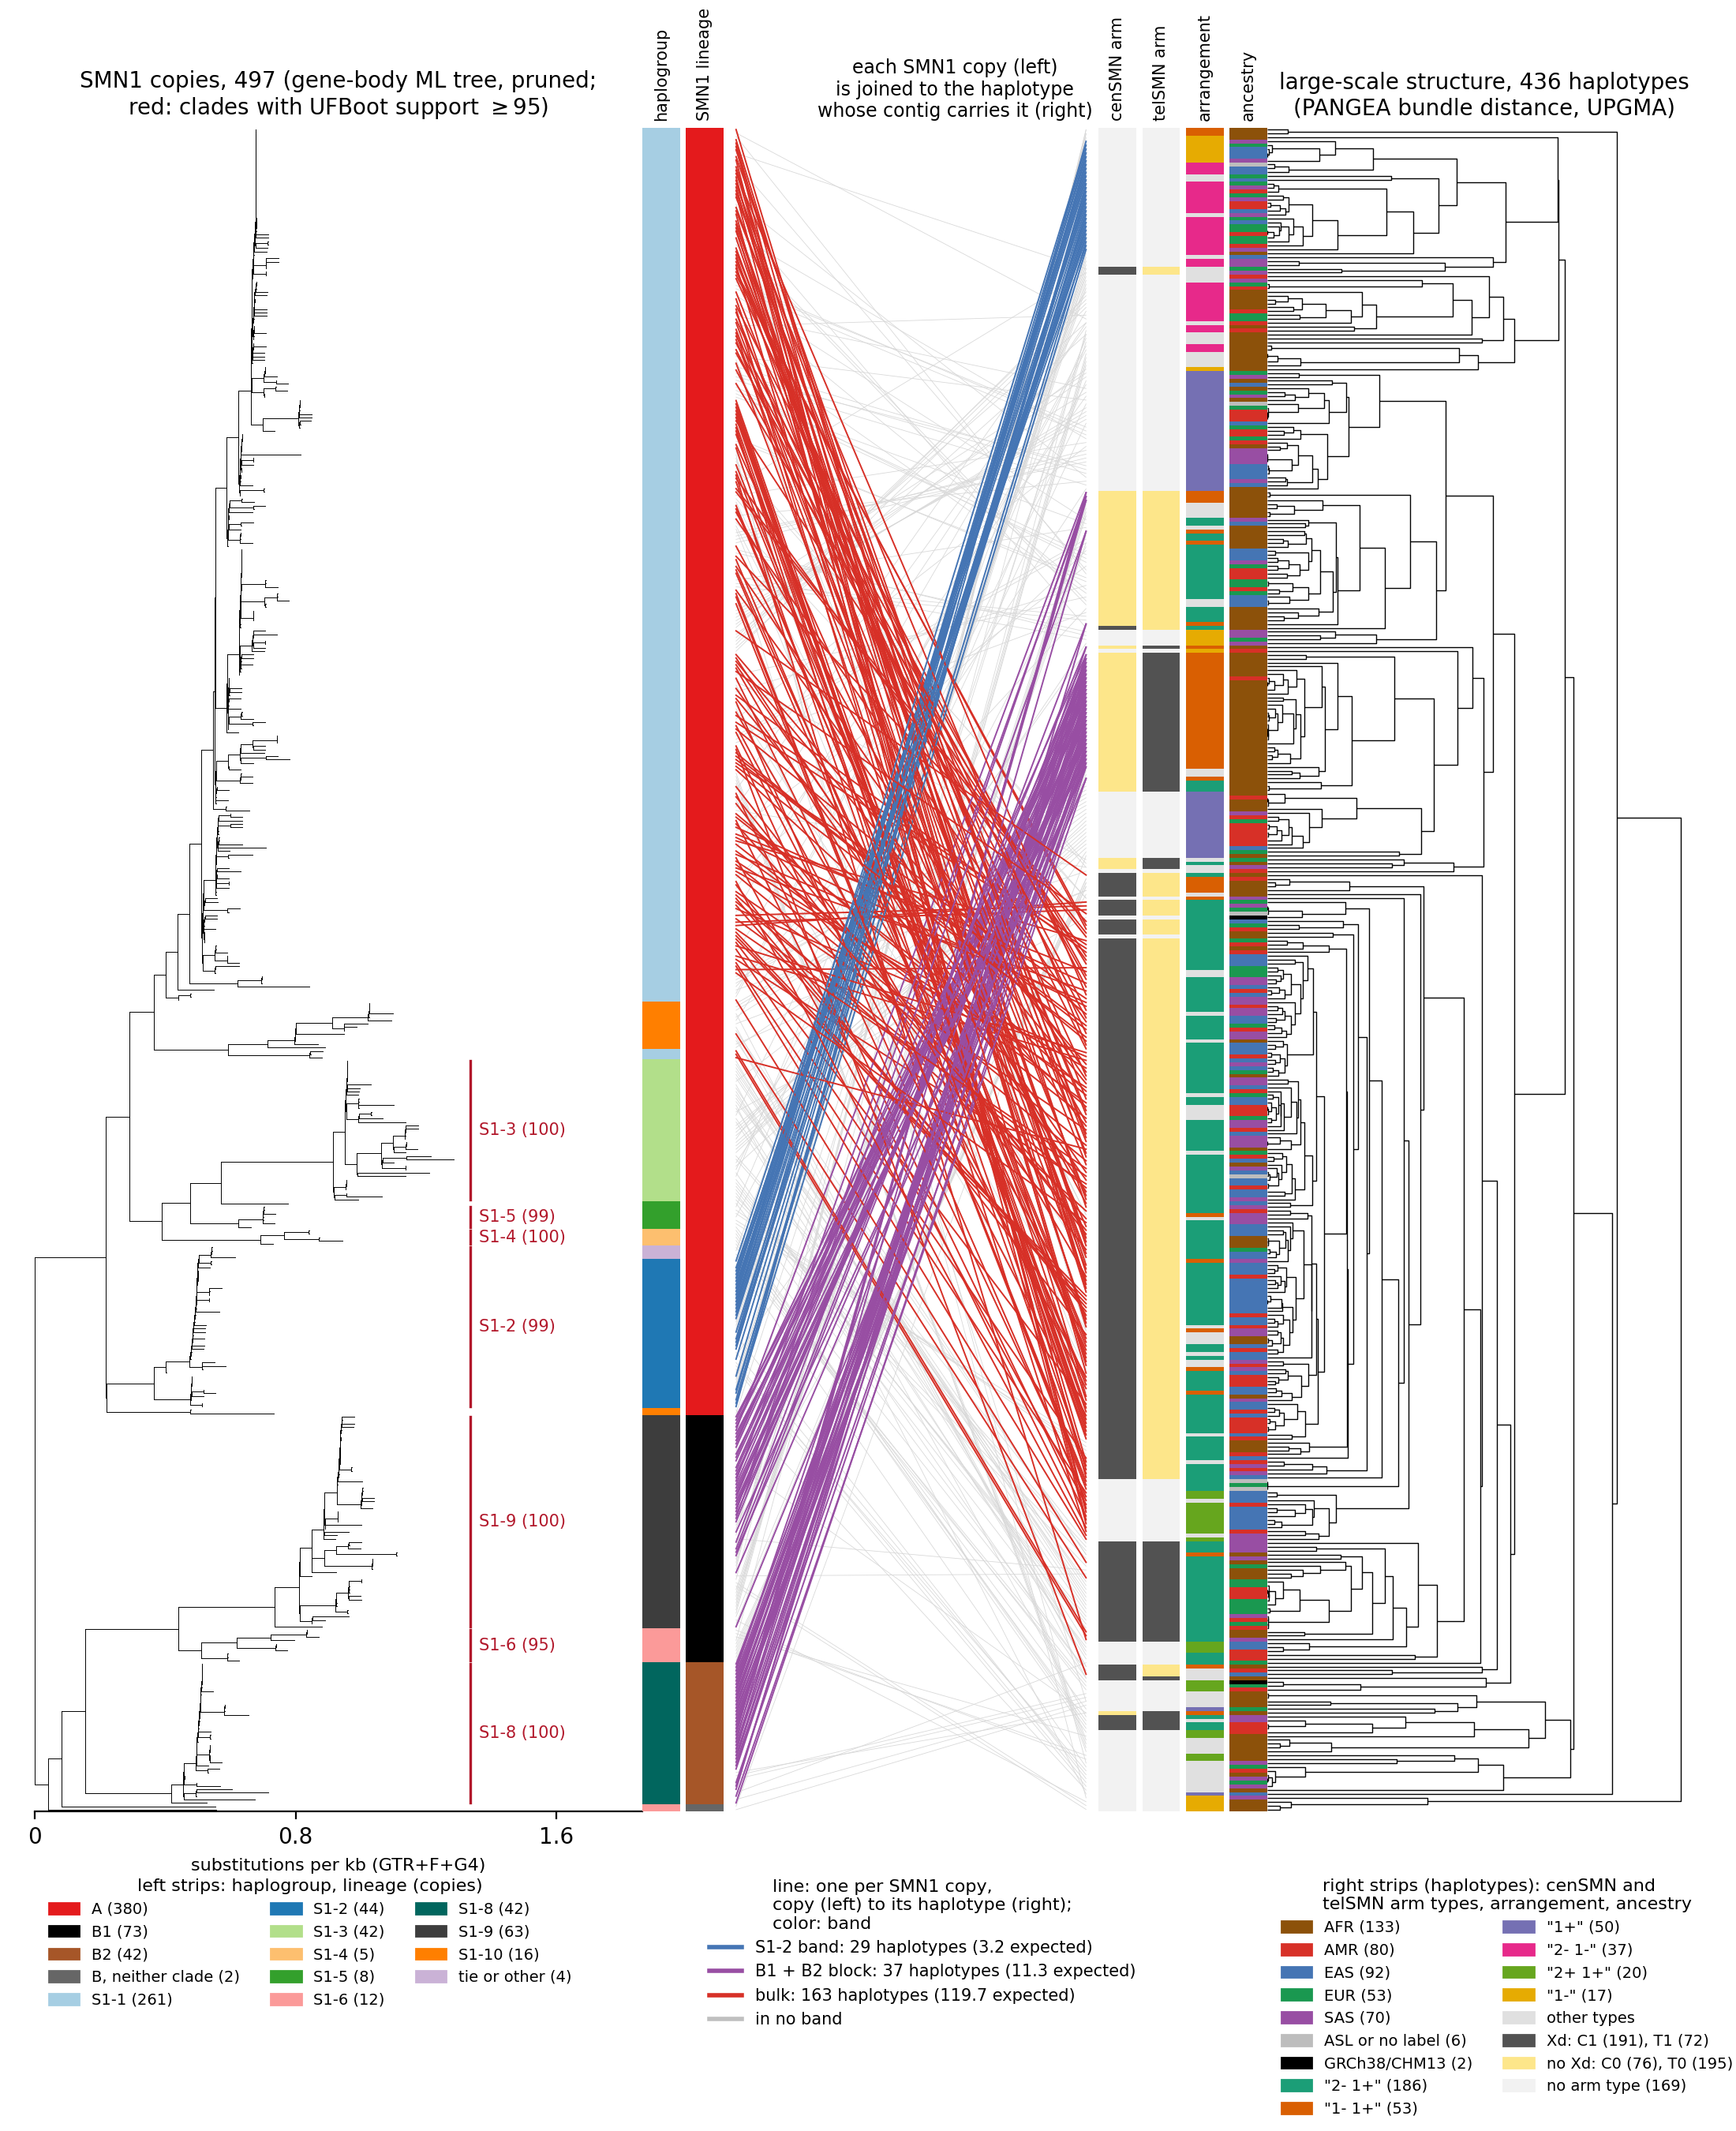
\includegraphics[width=\linewidth,height=0.64\textheight,keepaspectratio]{../figures/tanglegram_ml.png}
\caption{SMN1 sequence against large-scale structure for the \mlbHaps{} haplotypes that carry an SMN1 copy
(\nHapsResSMNone{} resolved haplotypes, GRCh38 and CHM13). The two trees have different leaves: on the left each leaf is
one SMN1 gene copy, on the right each leaf is one haplotype. Left, the gene-body maximum-likelihood tree
(main text, Fig.~\ref{fig:mltree}) pruned to these haplotypes' \mlbCopies{} SMN1 copies (the other \smnOneUnres{} of the tree's \smnOneAll{} SMN1 copies, all lineage A, sit on \smnOneUnresHaps{} unresolved haplotypes, which have no structural distance), leaves facing the middle, with strips for
each copy's Chen et al.\ haplogroup~\cite{chen2023} and lineage. Right, the UPGMA tree on PANGEA's bundle distance
between haplotypes, drawn mirrored so its leaves also face the middle, with strips for each haplotype's cenSMN and telSMN arm
types (Section~\ref{m:arms}; dark gray, the arm carries Xd, C1 or T1; yellow, it does not, C0 or T0; light gray, no arm type, the haplotype not being one of the \palPair{} with the palindrome; the legend counts the \afPairInTree{} pair haplotypes in this tree, the other \afPairOutTree{} carrying no SMN1 copy), arrangement type and continental group. Each SMN1 copy was cut from one haplotype's contig, so it belongs to exactly one haplotype: a line
joins the copy's leaf to the leaf of that haplotype. \mlbOneCopy{} haplotypes carry one SMN1 copy and have one line;
\mlbTwoCopy{} carry two and have two (\mlbOneCopy{} + 2\,$\times$\,\mlbTwoCopy{} = \mlbCopies{} lines). Red bars mark the
clades with ultrafast-bootstrap support (UFBoot, IQ-TREE's bootstrap approximation) $\ge$\setMLsup{} and at least \setMLmin{} SMN1 copies that define the sequence
clusters (support in brackets; supports are over the copies drawn here, so the S1-3 clade, support \mlThreeSup{} over all its \mlThreeN{} copies, shows \mlbThreeSup; the haplogroup legend counts every copy of a haplogroup; the S1-4 and S1-5 clades (support \mlbFourSup{} and \mlbFiveSup) hold only \mlbFourOwn{} and \mlbFiveOwn{} copies outside the smaller clades they contain; a bar spans the copies a clade holds outside smaller such clades, so S1-6's spans the
S1-6 copies outside the S1-9 clade). Lines are colored by band, a structure cluster and a sequence cluster (\setK{} structure clusters) sharing at least
\setMinOverlap{} haplotypes with Bonferroni $p<\setAlpha$: red, the bulk (SMN1 copies outside the supported clades,
mostly S1-1, on ``2-~1+''); blue, the S1-2 band; purple, the ``1-~1+'' haplotypes carrying B1
and B2; gray, no band.}
\label{fig:tangclus}
\end{figure}


\subsection{Inside an arrangement type, haplotypes that share an SMN1 haplogroup are closer in structure as well as in sequence (Fig.~\ref{fig:hgscatter})}\label{sec:hgscatter}
The clusters of pairs inside each arrangement type (Fig.~\ref{fig:scattype}) were tested against Chen et al.'s
haplogroups (Section~\ref{sec:chenhg}; step \texttt{26\_scatter\_lineage\_haplogroup.py}). A haplotype's haplogroup
make-up is the haplogroup families of its SMN1 copies, sorted and joined (for example S1-8+S1-9); the same make-up
implies the same lineage make-up. Of the \hsPairs{} pairs of haplotypes of the same type, \hsSameHg{} share a
haplogroup make-up and \hsSameLin{} a lineage make-up. Pairs that share a haplogroup make-up are closer on both axes:
median sequence distance \hsSeqSame{} against \hsSeqDiff{} differences per kb, and median structural distance
\hsStrSame{} against \hsStrDiff. Type by type, \hsTested{} of the \hsTypes{} types carried by ten or more haplotypes
can be tested (``1-~2+'' has one make-up only). In each, the same-make-up pairs are closer in structure (medians
\hsStrSameLo--\hsStrSameHi{} against \hsStrDiffLo--\hsStrDiffHi) and in sequence (\hsSeqSameLo--\hsSeqSameHi{}
against \hsSeqDiffLo--\hsSeqDiffHi), each at $p=\hsPfloor$, the floor of \hsShuf{} shuffles of the make-up labels
among the type's haplotypes. Kept to pairs of one make-up, the structure--sequence rank correlation inside a type falls
to \hsRhgLo--\hsRhgHi{} (from \hsRallLo--\hsRallHi{} over all pairs of the type) in every tested type but ``1-'',
where it rises (\hsRoneAll{} to \hsRoneHg). So the
clusters inside a type are largely haplogroup clusters, and the haplogroups are what tie structure and sequence
together there; this is the within-type side of the bands of Section~\ref{sec:bands}.

\begin{figure}[p]\centering
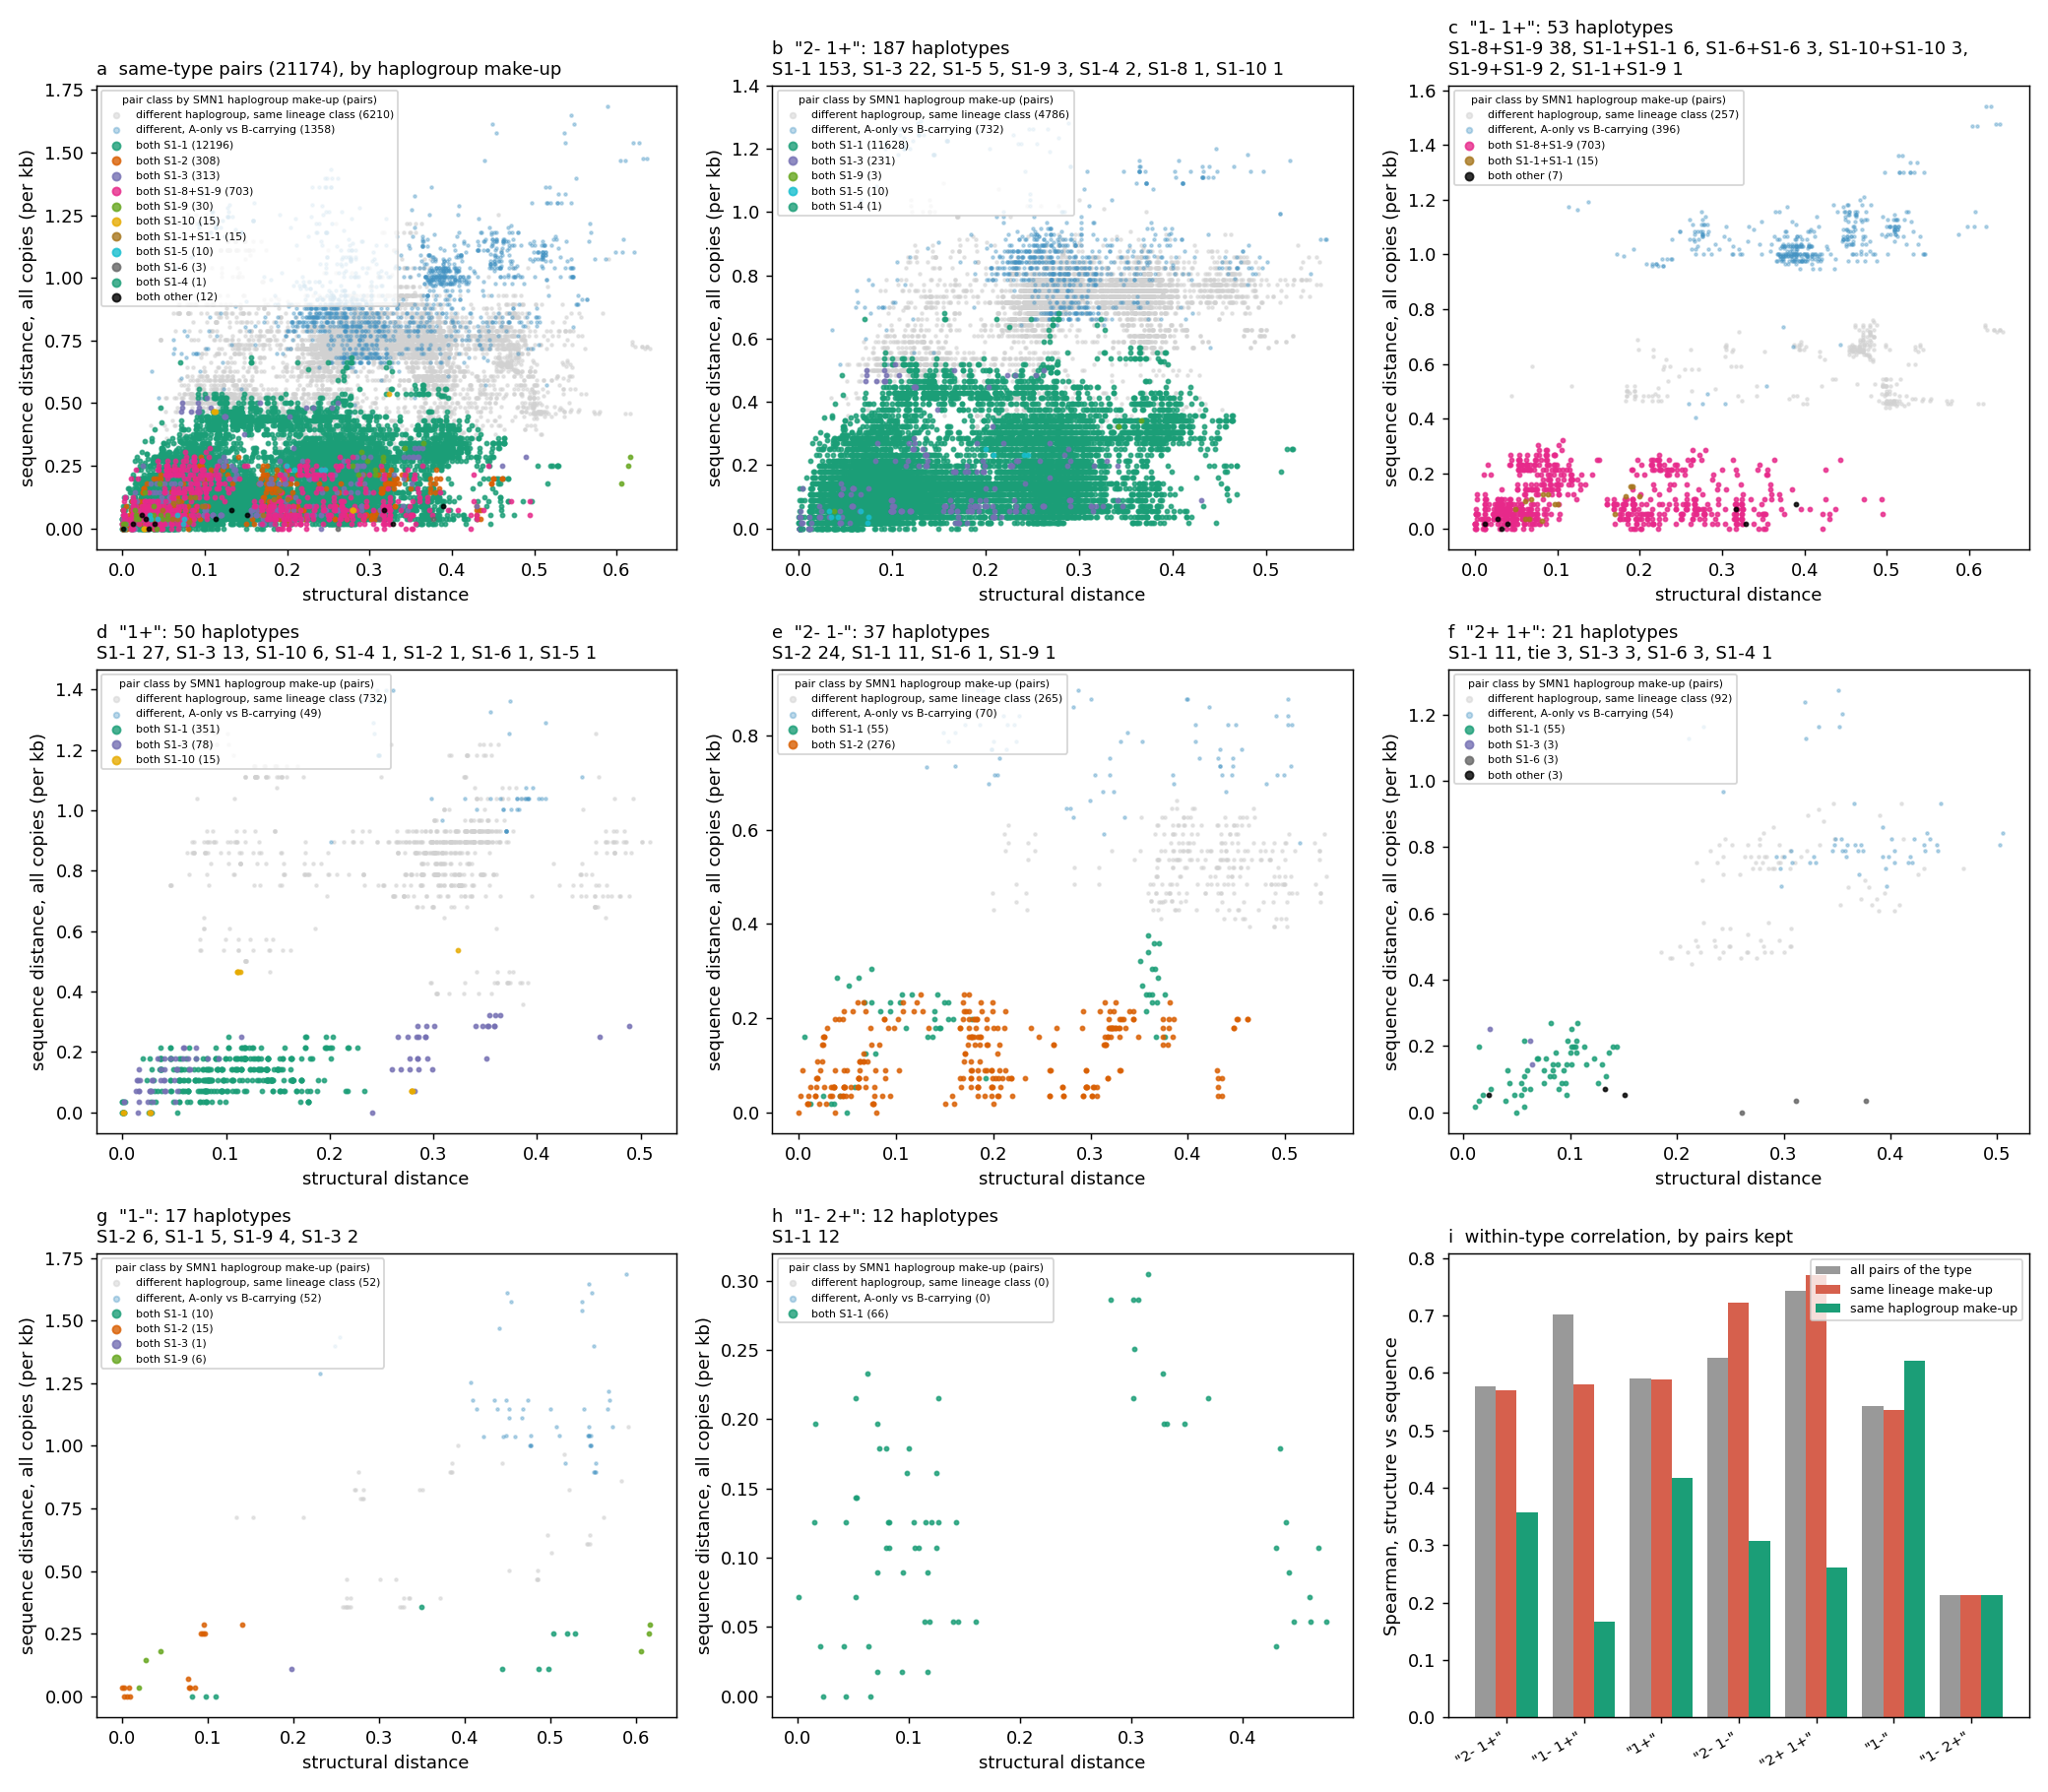
\includegraphics[width=\linewidth]{../figures/hap_scatter_hg.png}
\caption{Pairs of haplotypes of the same arrangement type, by structural distance (x) and sequence distance of all
their SMN copies (y, differences per kb), colored by SMN1 haplogroup make-up: a color, both haplotypes have that
make-up; light gray, different make-ups within one lineage class; blue, one haplotype carries only A copies and the
other a B copy. \textbf{a}, all \hsPairs{} same-type pairs; \textbf{b--h}, one panel per type with ten or more
haplotypes, titled with its make-ups and their counts. \textbf{i}, within-type rank correlation of structure and
sequence over all pairs of the type, over pairs of the same lineage make-up, and over pairs of the same haplogroup
make-up. Drawn by \texttt{26\_scatter\_lineage\_haplogroup.py}.}
\label{fig:hgscatter}
\end{figure}

\section{SMN1 lineages A and B, and the sub-lineages B1 and B2}\label{sec:lineages}
\subsection{The lineages are the two halves of the maximum-likelihood tree}\label{sec:apart}
Lineages are defined on the maximum-likelihood tree of the gene body (Section~\ref{m:lineages}, Fig.~\ref{fig:mltree};
step \texttt{05\_\allowbreak lineages.py}). Rooted on the orangutan copy, the human copies form one clade whose two child clades
are the two halves: \emph{lineage B} is the SMN1 copies of the half that holds the \cpe{} copies (\linB{} SMN1 copies
and \mlBsideHtwentyone{} h21 copies, support \mlIsup), and \emph{lineage A} the SMN1 copies of the other half (\linA,
with every SMN2 copy; support \mlIIsup). Within B's half, exactly two clades have support $\ge$95
and lie in no larger such clade: \emph{B1} is the SMN1 copies of the one that holds the h21 copies (\linBone{} copies with
\mlBhH{} h21 copies, support \mlBhSup), and \emph{B2} the SMN1 copies of the other (\linBtwo{} copies, support
\mlEightSup); the \linBnone{} remaining B copies are in neither. The node that joins B1 and B2 alone (\mlBBjoinCopies{}
copies) has support \mlBBjoinSup: by p-distance B2 is nearer A (\gsABtwo{} differences per kb) than it is to B1
(\gsBoneBtwo; Section~\ref{sec:grpdist}).

\subsection{Lineage B is exactly Chen et al.'s S1-6, S1-8 and S1-9 haplogroups (Table~\ref{tab:chenhg})}\label{sec:chenhg}
Our copies were matched to Chen et al.'s haplogroups~\cite{chen2023} by two independent routes (step
\texttt{11\_chen\_\allowbreak haplogroups.py}). Chen et al.'s ``haplotype'' is one gene copy (one SMN1 or SMN2 sequence), not a
chromosome. Chen et al.\ defined their haplogroups by reading monophyletic groups off a neighbor-joining tree of
such copies, and Paraphase assigns a new copy to the haplogroup of the most similar representative sequence; here copies are
assigned from their variant table.

\textbf{Copy by copy:} their supplementary Table S6 lists the variants shared within each haplogroup
(\hgSixVar{} variants, \hgSixSnv{} of them single-base, on GRCh38). \hgPlaced{} of the single-base ones fall inside the
aligned copies (\hgPlacedOne{} on the SMN1 locus, \hgPlacedTwo{} on the SMN2 locus), and the GRCh38 base at every one
is the reference base the table gives. Each SMN1 copy was genotyped at these sites and given the haplogroup whose
variant set it matches best: the Jaccard index of the copy's alternative bases and the haplogroup's listed variants,
at the sites where the copy has a base. Ties are kept (\hgTied{} of the \hgCopies{} SMN1 copies, \hgWithinTie{} of them between
subgroups of one family). The lead of the best haplogroup over the next has a median of \hgMarginB{} for B copies and
\hgMarginA{} for A copies, so the calls among the A haplogroups are the less certain.

\textbf{Person by person:} for the \hgPeople{} people in both Chen et
al.'s Table S3 and our tree, our lineage counts were set against the haplogroup names their method gave.
\begin{itemize}
\item \textbf{B is S1-6, S1-8 and S1-9; A is everything else.} B1 holds all \hgNineB{} copies of the S1-9 family
(S1-9 \hgNinePB, S1-9c \hgNineCB, S1-9d \hgNineDB) and \hgBoneSix{} of the \hgSixB{} S1-6 copies; B2 holds all
\hgEightB{} S1-8 copies; the \hgBnoneSix{} B copies in neither clade are S1-6. No copy of these three haplogroups is in
A, and every other haplogroup (S1-1 to S1-5, S1-10) is in A only. The worst B match has a Jaccard index of
\hgBMinJac{}, and no B copy is tied between haplogroups.
\item \textbf{The marker:} \hgMkNine{} S1-9 copies and \hgMkEight{} S1-8 copies carry \cpe, and no other copy
(Section~\ref{sec:marker}).
\item \textbf{SMN2's nearest SMN1:} the S1-10 copies are the A copies nearest SMN2 (mean \hgTenToTwo{} differences
per kb, against \hgAToTwo{} for all A), as Chen et al.\ found; S1-9 copies are \hgNineToTwo{} from SMN2.
\item \textbf{Person by person:} our B count equals the person's number of S1-6, S1-8 and S1-9 copies in all
\hgPeopleNineSix{} people.
\end{itemize}
\hgWithinTie{} A copies tie between S1-2 and S1-2c, which differ only downstream of the gene, and \hgTieA{} A copies
match no haplogroup better than another; neither touches the A/B question. The lineage split is therefore not a new
grouping: it is the deepest division among Chen et al.'s haplogroups, and their common African two-copy allele
(S1-8 with S1-9d) is a B2 copy with a B1 copy. What the assemblies add is where those copies sit
(Section~\ref{sec:posstrand}).

\begin{table}[htbp]\small\centering
\caption{SMN1 copies of each Chen et al.\ haplogroup family (by the copy-level match) in lineages A and B, how many
carry \cpe, and their mean distance to the SMN2 copies (differences per kb). Families: S1-1 includes S1-1c, and so
on. ``tie'': equally good matches across families. Written by \texttt{40\_numbers.py} from
\texttt{results/sv/chen\_hg\_copies.tsv}.}\label{tab:chenhg}
\begin{tabular}{@{}lrrrr@{}}\toprule
Haplogroup family & A & B & \cpe{} & To SMN2\\\midrule
\tabChenHg
\bottomrule\end{tabular}
\end{table}

\subsection{B1 is the copy group furthest from SMN2, and B2 lies nearer A than it does to B1 (Fig.~\ref{fig:grpdist}, Table~\ref{tab:grpdist})}\label{sec:grpdist}
Every pair of copies among lineage A (\linA{} copies), lineage B (\linB) and SMN2 (\gdNTwo), with the \gdNHtw{} h21
hybrids beside them, is compared over the same \nGeneCols{} gene-body columns (Section~\ref{sec:compared}), counting
differences over the bases both copies have (on average \gdBases{} per pair; step \texttt{10\_group\_distances.py}).
The same comparison with B split into B1 and B2 is in \texttt{results/sv/group\_pair\_distances\_sub.tsv}.
\begin{itemize}
\item \textbf{Within each group} (differences per kb, mean): B2 is the most uniform (\gsBtwoBtwo), then B1
(\gsBoneBone), A (\gsAA) and SMN2 (\gdTwoTwoMean). B as a whole is \gdBBMean, because it holds two sub-lineages
\gsBoneBtwo{} apart.
\item \textbf{A against SMN2} is the closest pair of the three groups: mean \gdATwoMean{} (\gdATwoDiffs{} differences per
pair), range \gdATwoMin--\gdATwoMax; \gdATwoBelow\% of these pairs are closer than the 95th percentile of
within-group distances.
\item \textbf{A against B}: mean \gdABMean{} (\gdABDiffs{} differences), range \gdABMin--\gdABMax; by sub-lineage A is
\gsABtwo{} from B2 and \gsABone{} from B1, so B2 is nearer A than it is to B1 (\gsBoneBtwo).
\item \textbf{B against SMN2} is the furthest: mean \gdBTwoMean{} (\gdBTwoDiffs{} differences), B1 \gsBoneTwo{} and B2
\gsBtwoTwo; the closest B--SMN2 pair (\gdBTwoMin) is further apart than the median A--SMN2 pair (\gdATwoMed), and
\gdBTwoBelowFine\% of B--SMN2 pairs are closer than the 95th percentile of within-group distances (shown as 0\% in
Table~\ref{tab:grpdist} after rounding).
\item \textbf{Copy by copy} (Fig.~\ref{fig:grpdist}c,d): no B copy is on average nearer SMN2 than the other B copies
(\gdBNearTwo{} of \linB), \gdBNearA{} is nearer A, and no SMN2 copy is nearer A than SMN2 (\gdTwoNearA{} of \gdNTwo).
No A copy is nearer B than A (\gdANearB), and \gdANearTwo{} (\gdANearTwoHap) is nearer SMN2 than A.
\item \textbf{h21} hybrids are on average nearest SMN2 (\gdTwoHtwMean), then B (\gdBHtwMean) and A (\gdAHtwMean);
their wide spread (within h21 up to \gdHtwHtwMax) fits copies that mix the two genes.
\end{itemize}
By raw difference counts, then, A and SMN2 are the nearest pair, and B1 is the group furthest from SMN2. These counts do
not say why: shared ancestry, or gene conversion between A and SMN2 copies, would give the same pattern
(Section~\ref{sec:history}). Distances are p-distances, uncorrected for repeated changes at one site; every
difference counts once (a long insertion counts as many); pairs share copies and are not independent, so the ranges
and shares are descriptive.

\begin{figure}[htbp]\centering
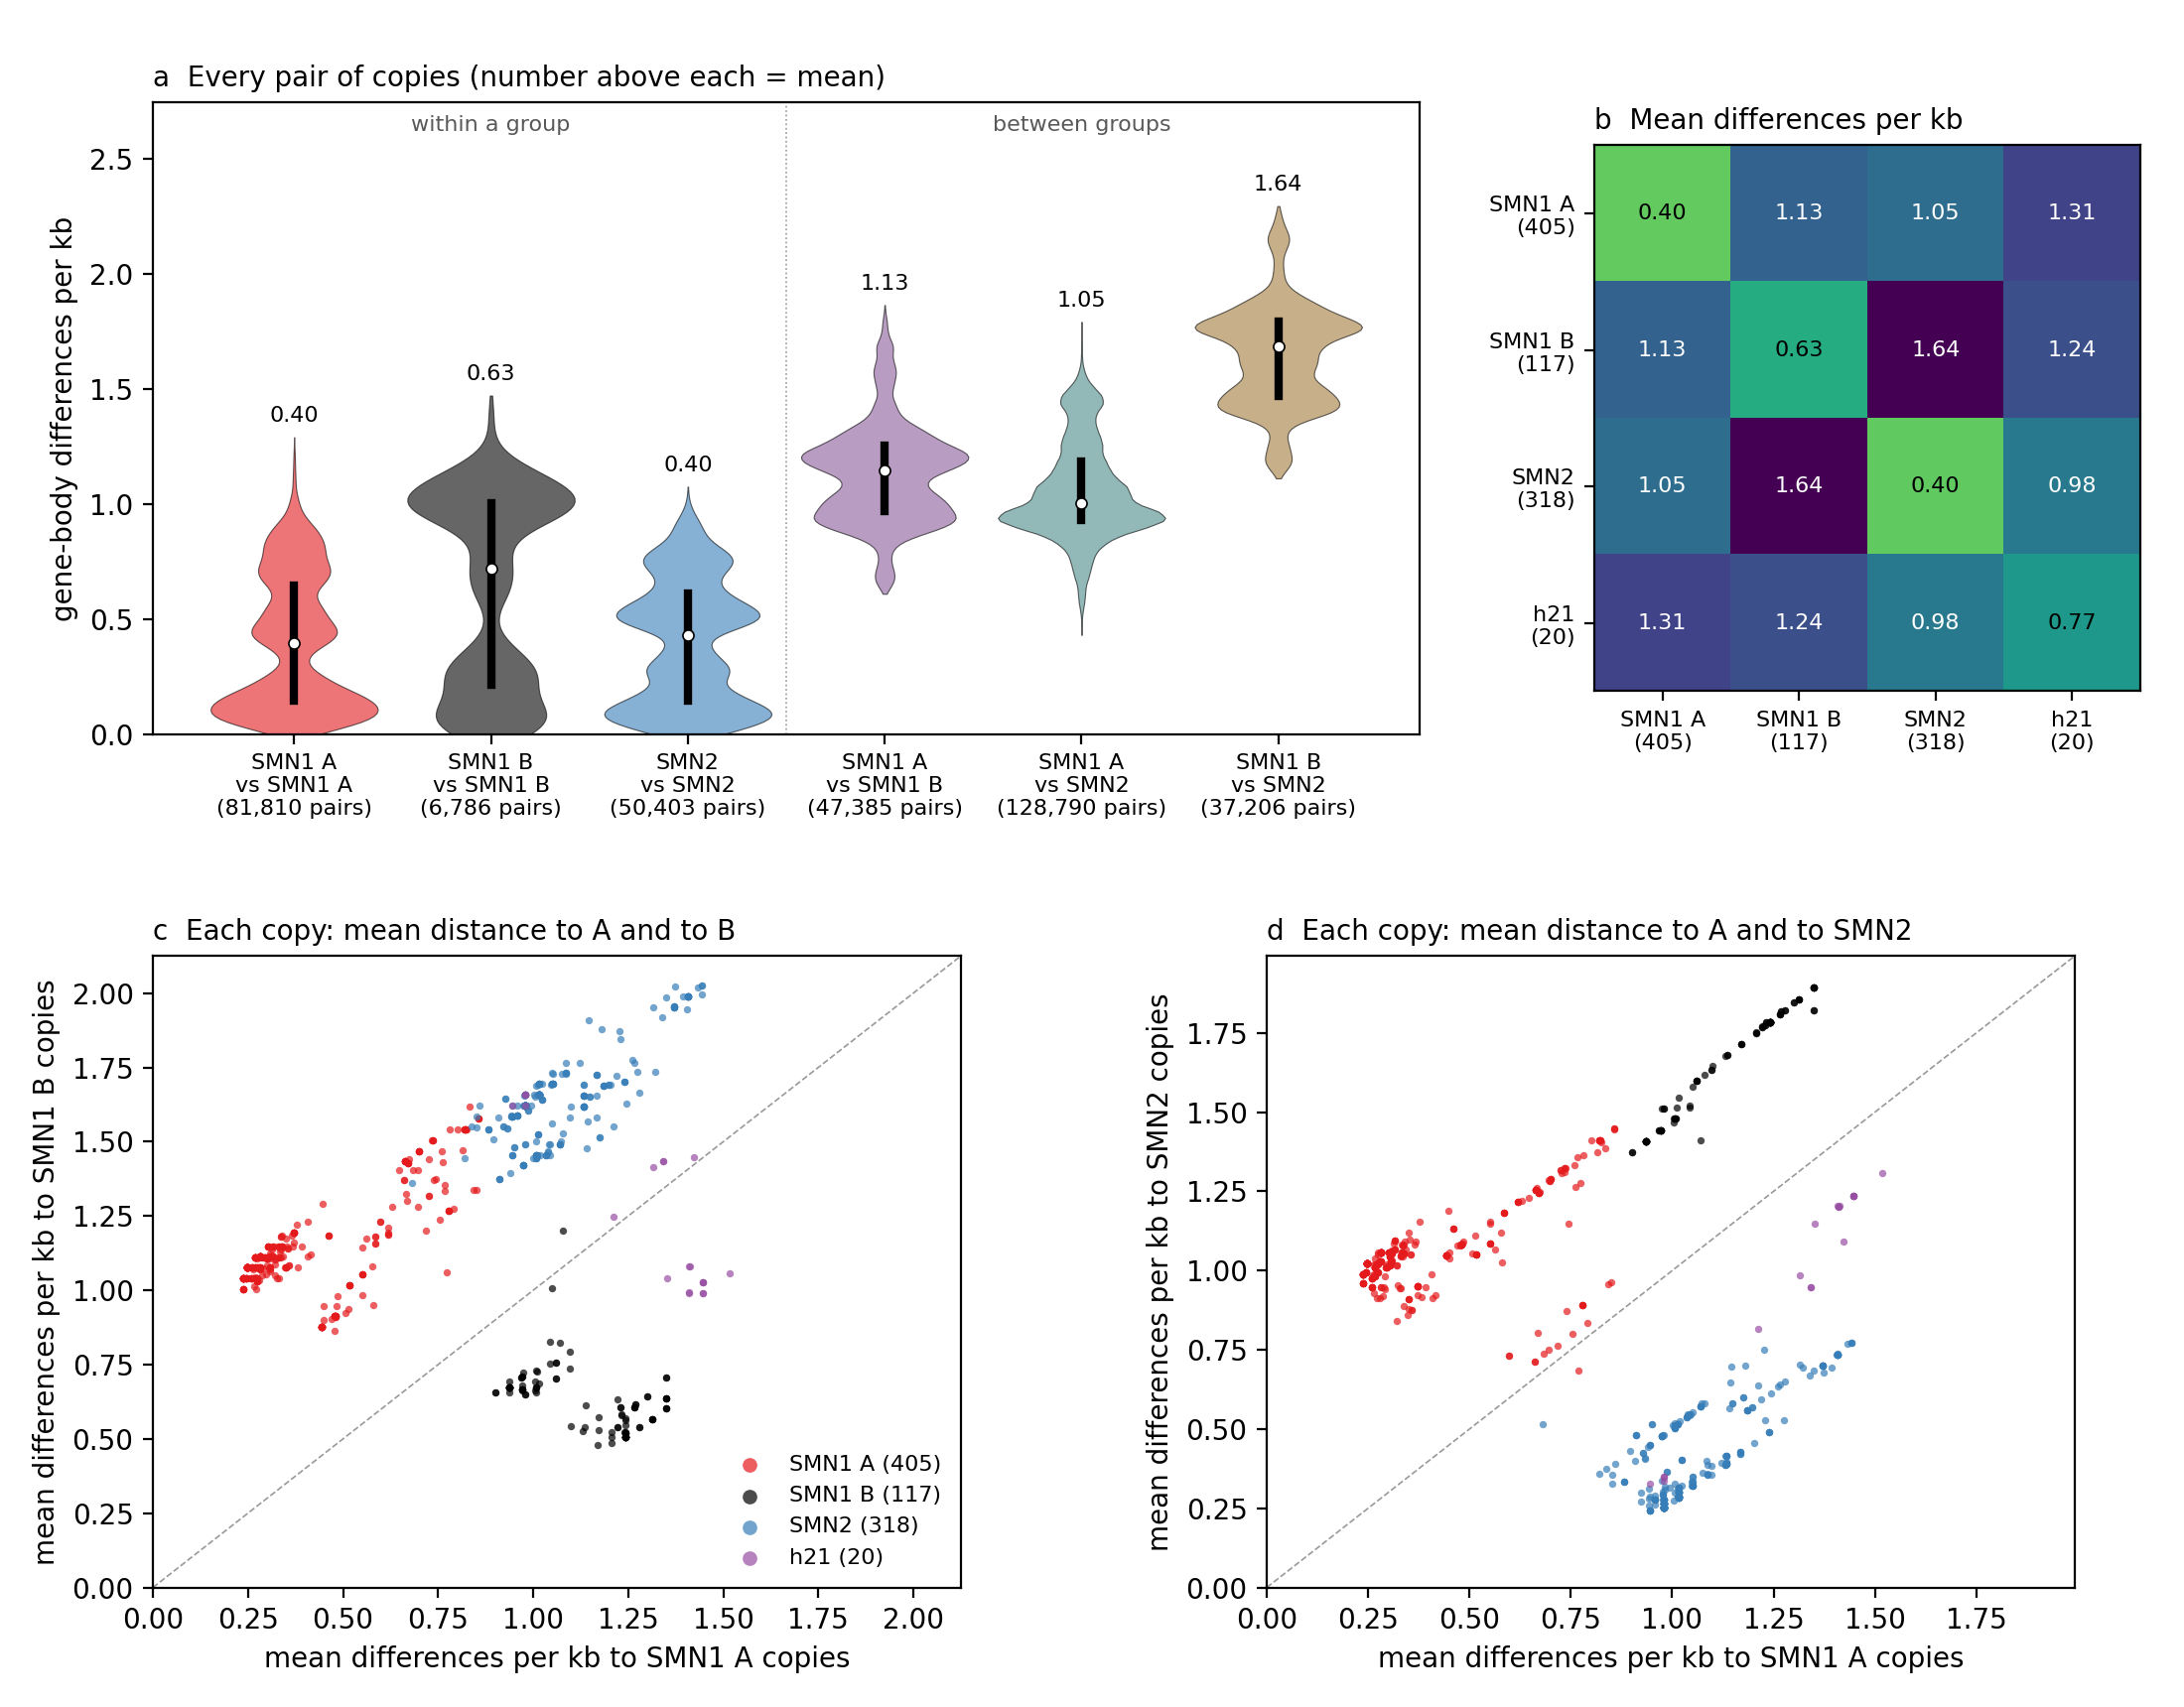
\includegraphics[width=\linewidth]{../figures/group_distances.png}
\caption{Gene-body distances between every pair of copies of SMN1 lineage A (red), SMN1 lineage B (black) and SMN2
(blue), with h21 hybrids (purple); colors as in Figs.~1--5. \textbf{a}, distribution of the distance over all pairs within each group and
between each pair of groups (violin; bar, interquartile range; dot, median; number, mean; pair counts under each).
\textbf{b}, mean distance for every pair of groups, h21 included. \textbf{c}, each copy's mean distance to the A
copies against its mean distance to the B copies; \textbf{d}, the same against the SMN2 copies (a copy's distance to
itself left out); dashed line, equal distance. B is not split into B1 and B2 here. Drawn by
\texttt{10\_group\_distances.py} from \texttt{results/sv/copies.aln.fa}.}
\label{fig:grpdist}
\end{figure}

\begin{table}[htbp]\small\centering
\caption{Gene-body distance between copies, differences per kb, for every pair of groups: pairs compared, mean,
median, 5--95th percentile, range, mean differences per pair; for pairs of different groups, the net distance (mean
minus the average of the two within-group means) and the \% of pairs closer than the larger of the two within-group
95th percentiles. Written by \texttt{40\_numbers.py} from \texttt{results/sv/group\_pair\_distances.tsv}.}\label{tab:grpdist}
\begin{tabular}{@{}lrrrrrrrr@{}}\toprule
Groups & Pairs & Mean & Median & 5--95\% & Range & Diffs & Net & \% within\\\midrule
\tabGrpDist
\bottomrule\end{tabular}
\end{table}

\subsection{Two sites separate A from B in every copy; none lies in the coding sequence (Fig.~\ref{fig:absites})}\label{sec:absites}
The lineages differ at \abCols{} gene-body columns, where the commonest state in A differs from the commonest state in B
(a gap counts as a state). Adjacent columns of one insertion or deletion merge into one event, leaving \abEvents{}
events: \abSNV{} base changes and \abIndel{} insertions or deletions (step \texttt{23\_ab\_sites.py}).
\begin{itemize}
\item \textbf{How cleanly they separate.} The \emph{separation} of an event is the share of copies carrying their own
lineage's state, taken in the lineage where that share is lower. At \abNearFixed{} events it is at least 90\%
(\emph{near-fixed}), and at \abPerfect{} it is 100\% (no copy of either lineage carries the other state):
chr5:\abPerfOnePos{} (\abPerfOneKind{} in the 5$'$ untranslated part of exon~1, \abPerfOneC; A's base on
\abPerfOneA{} of \linA{} A copies, B's on \abPerfOneB{} of \linB{} B copies) and chr5:\abPerfTwoPos{}
(\abPerfTwoKind{} in intron~1; \abPerfTwoA{} and \abPerfTwoB).
\item \textbf{Where.} Most events lie in intron~1 (\abIntronOne) and intron~6 (\abIntronSix); \abExonEvents{} touch an
exon, the one in exon~1 above and c.*211\_*212del in the 3$'$ untranslated part of exon~8. None lies in the coding
sequence.
\item \textbf{SMN2.} At \abTwoA{} events SMN2 carries A's state and at \abTwoB{} B's, which fits A and SMN2 being the
nearest pair (Section~\ref{sec:grpdist}), though these sites are only part of that distance.
\end{itemize}
The \evAB{} sites of the history (Section~\ref{sec:history}) are the near-fixed events less the one insertion or
deletion among them, since the ape bases are read at single-base sites. The lineages were cut from a tree built on this same alignment, so how cleanly a site separates
them is partly built in; copies outside the tree, or reads, would be needed to test these sites as lineage markers.

\begin{figure}[htbp]\centering
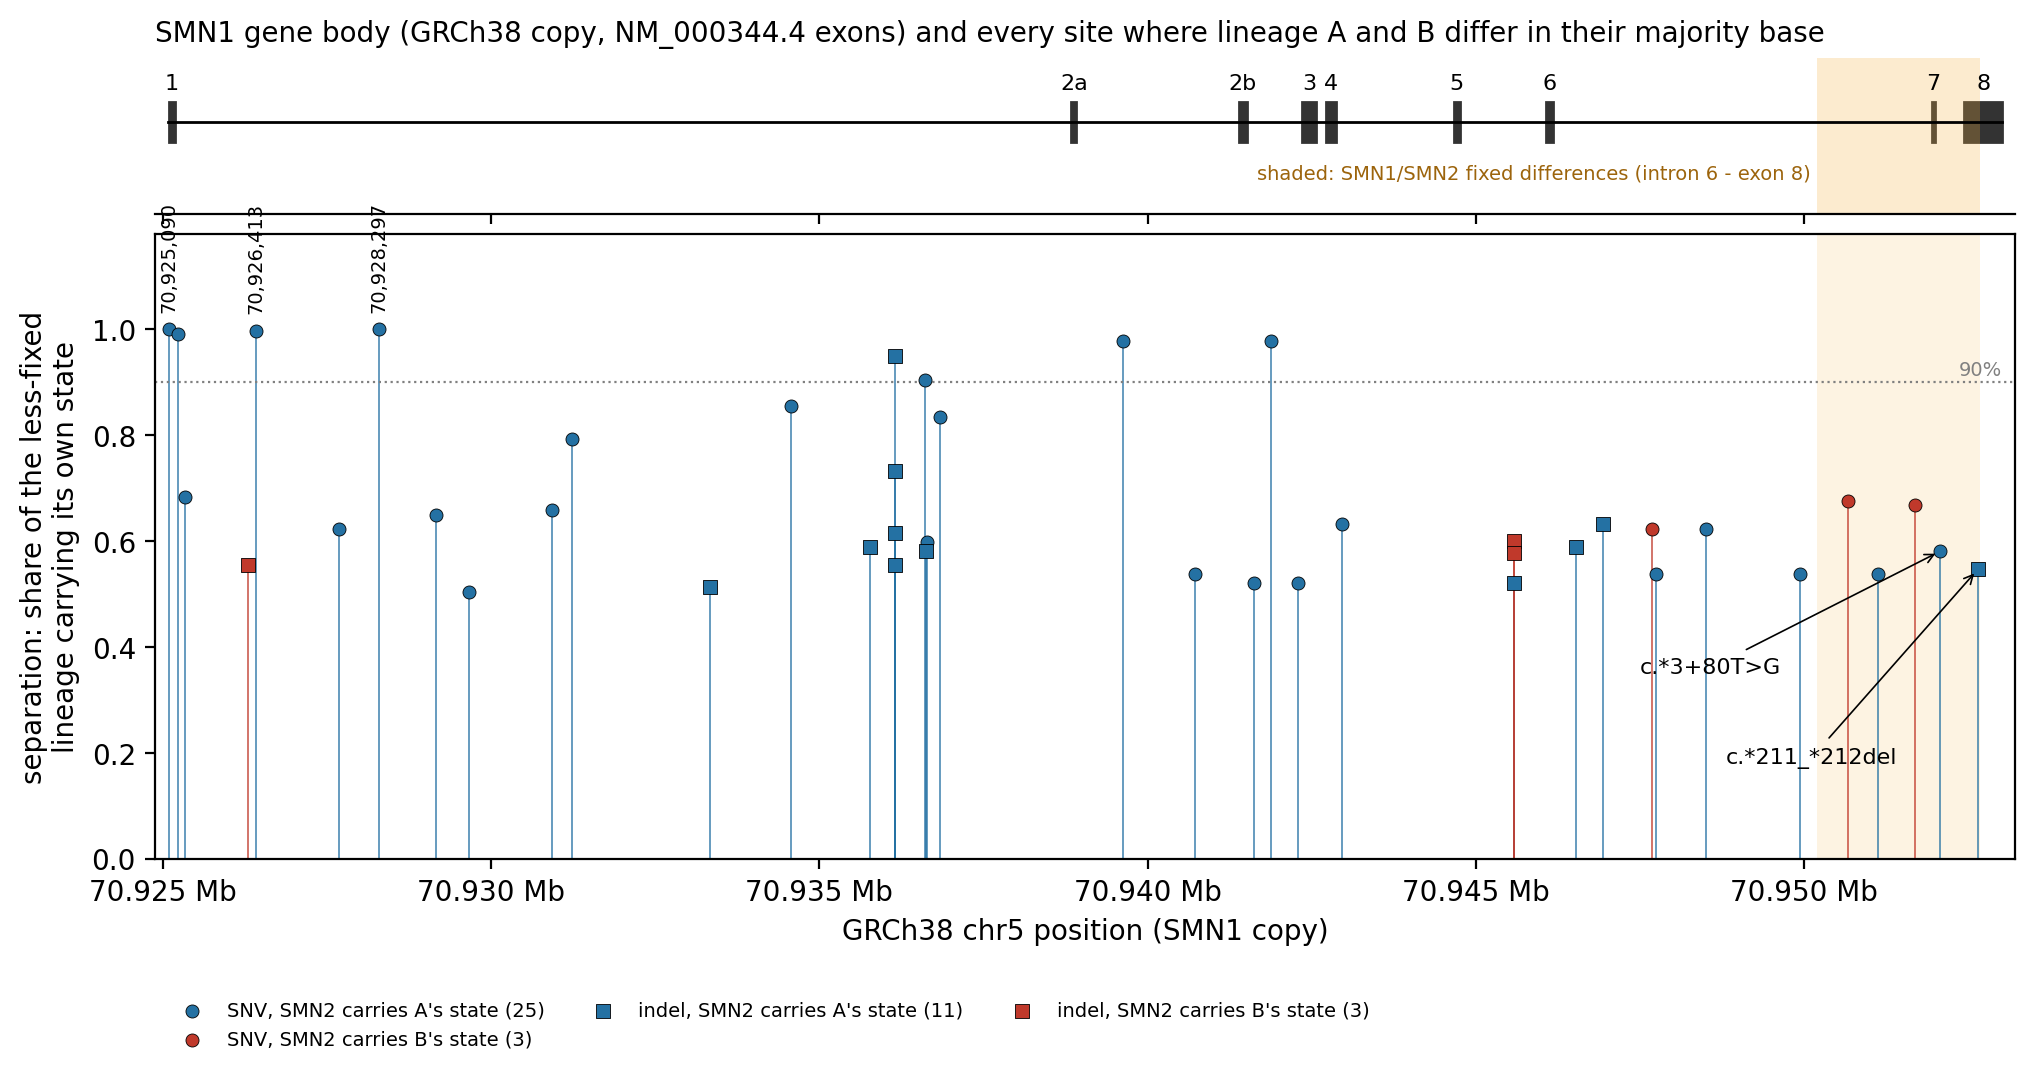
\includegraphics[width=\linewidth]{../figures/ab_sites.png}
\caption{Every gene-body site where the commonest state of lineage A differs from that of lineage B, drawn along the
SMN1 gene (GRCh38 chr5 coordinates) over the exons of NM\_000344.4: base changes and insertions or deletions, their
height the separation (share of the less-fixed lineage carrying its own state), colored by whose state SMN2 carries;
\cpe{} and c.*211\_*212del are labeled. Drawn by \texttt{23\_ab\_sites.py} (\texttt{results/sv/ab\_sites.tsv},
\texttt{results/sv/ab\_site\_events.tsv}).}
\label{fig:absites}
\end{figure}

\subsection{The duplication marker c.*3+80T>G tags B1 and part of B2}\label{sec:marker}
\cpe{} lies in intron~7, 80 bases after the end of exon~7 (chr5:70{,}952{,}074 on the GRCh38 SMN1 copy), so it does not
change the protein. Luo et al.\ sequenced \emph{SMN1} in Ashkenazi Jewish and African American carriers of duplication
alleles and reported six variants on the major Ashkenazi duplication allele: g.27134T>G in intron~7 (\cpe{}) and
g.27706\_27707delAT in exon~8 (c.*211\_*212del), which in every case they examined lay together on one \emph{SMN1} copy, and
four changes in introns~1, 2a and~6 found with them in both groups. g.27134T>G was on 49 of 99 Ashkenazi duplication
carriers, and on duplication alleles in every group they tested, though specific to them only in their Asian
sample; finding it in a person with two \emph{SMN1} copies sharpens the residual risk of being a silent 2+0
carrier~\cite{luo2014}. Later assays genotype the two with copy number~\cite{feng2017,milligan2021,mikhalchuk2025}.
Luo et al.'s Table~4 gives GRCh37 positions. Shifted by \luoShift{} bases, the shift that puts their exon-8 deletion at
c.*211 of the GRCh38 copy and at which each of their reference bases is the GRCh38 base, five of the six fall on
lineage B1 (step 23b, \texttt{results/sv/luo\_variants.tsv}): each is on \luoBoneLo--\luoBoneHi{} of the \linBone{} B1
copies and on no A or SMN2 copy, while B2 carries only the intron-7 change (\luoBtwoMk{} copies, without the
deletion), so here the two do not always travel together. The sixth, an intron-1 G>T at the end of a run of G next to
the run of 14 T that ends at \rdUnresSite{} and leaves one A/B site unresolved in the apes (Section~\ref{sec:history}), is on no copy as written; \luoIntronOneB{} B1 copies carry that run of G
shortened by one base at its other end, which may be the same change placed differently, and we leave it open. The
duplication haplotype Luo et al.\ described is thus, as far as these sites show, the haplotype of B1.
It tags only some duplication alleles: Chen et al.\
report that it carries a silent-carrier risk of 1.7--3.0\%, against 88.5\% for the S1-8 with S1-9d haplogroup pair, and
Mikhalchuk et al.\ found it in a small share of Russian duplication carriers~\cite{chen2023,mikhalchuk2025}. Here it is
on \linBoneMk{} of the \linBone{} B1 copies, \linBtwoMk{} of the \linBtwo{} B2 copies and no A copy: it marks
sub-lineage B1 nearly completely and B2 only in part, so a two-copy allele made of B2 copies, or a B1 copy without it,
is missed.

\subsection{Copy order and strand: A is telomeric, B1 centromeric and reversed, B2 telomeric and forward}\label{sec:posstrand}
A \emph{copy} is one SMN gene in the window: an SMN1, SMN2, hybrid (h12, h21) or $\Delta$7--8 copy (Section~\ref{sec:compared}). A copy's \emph{copy order} is which of the window's SMN genes it is, all of them
counted, from the centromeric end: \emph{centromeric} is the first copy from the centromeric end, \emph{telomeric} the last, \emph{middle} any
between, and \emph{single} the only SMN copy of the window. Copy order is counted over the whole window, so it is not the same as the cenSMN and telSMN slots of the arms of the \RU{A} pair (Section~\ref{sec:palindrome}); it is read on resolved haplotypes only. The main text and Fig.~\ref{fig:mltree} group copies by arm instead (Section~\ref{m:cen}); on the haplotypes with the pair the two agree, \coCenFirst{} of the \coCenN{} cenSMN-arm copies being first by copy order and \coTelLast{} of the \coTelN{} telSMN-arm copies last, while copy order also places the copies of haplotypes without the pair. A copy's
\emph{strand} is its orientation on the GRCh38-oriented window. Both are labels taken from the assembly, outside the
sequence comparison: every copy went into the alignment on the SMN1-gene strand, so neither label can shape the tree,
and an association between them and the lineages is not built in.

\textbf{The copies behind the counts.} Of the \linA{} A copies, \linACen{} are centromeric, \linATel{} telomeric (the
\linRef{} reference copies of GRCh38 and CHM13 among them, both forward), \linASingle{} single, \linAMid{} middle, and
\linAUnres{} sit on unresolved haplotypes and have no copy order. Of the \linB{} B copies, \linBCen{} are centromeric,
\linBTel{} telomeric and \linBSingle{} single, so none is a middle copy or on an unresolved haplotype; B1 is \linBoneCen{} centromeric, \linBoneTel{} telomeric and
\linBoneSingle{} single, and B2 \linBtwoCen{} centromeric and \linBtwoTel{} telomeric. The copy-order test below uses
the \linPosN{} centromeric and telomeric copies.

\textbf{Copy order.} A is telomeric in \linATel{} copies against \linACen{} centromeric. B as a whole is found in both
places, but its sub-lineages are not: B1 against B2, centromeric against telomeric, two-sided Fisher exact
$p=$\,\linSubPpos. On the \linMixHaps{} haplotypes with one B1 and one B2 copy (all ``1-~1+'', \linMixAfr{} of them
AFR), B1 is centromeric and reversed on \linMixBoneCenRev{} and B2 telomeric and forward on \linMixBtwoTelFwd.

\textbf{Strand mostly follows copy order, with one exception.} Every centromeric B1 copy is reversed (\linBoneCenRev{} of
\linBoneCen) and every telomeric B2 copy forward (\linBtwoTelFwd{} of \linBtwoTel). In A, \linACenRev{} of the
\linACen{} centromeric copies are reversed, and \linATelFwd{} of the \linATel{} telomeric copies forward: the first
copy of a head-to-head inverted pair reads reversed and the last forward. The exception is the \linATelRev{} telomeric
A copies that are reversed: \linATelRevTwoMOneM{} of them are on ``2-~1-'' and \linATelRevTwoPOneM{} on ``2+~1-''
haplotypes, where the SMN1 copy is not the forward member of a head-to-head pair. \linATelRevBand{} of them lie on the \linBandTwoN{} haplotypes of the S1-2 band
(Section~\ref{sec:bands}), one on each.

\textbf{How far to trust it.} Copy order does not define a lineage: \linBoneTel{} B1 copies are telomeric, \linBtwoCen{}
B2 copies centromeric, and \linACen{} A copies centromeric. \linBAfr{} of the \linB{} B copies are from AFR donors
(outside AFR, \linBNonAfrPops), so the association is mixed with ancestry and cannot be tested elsewhere. The Fisher
test treats copies as independent, though two copies of one haplotype, and haplotypes of one person, are not.

\subsection{Lineage B in populations, haplotypes and arrangements (Fig.~\ref{fig:lindetail}, Tables~\ref{tab:lincomp}--\ref{tab:linpop})}\label{sec:lindetail}
Every count here is a cross-tabulation written by \texttt{06\_lineage\_detail.py} or \texttt{40\_numbers.py}, with the
caveats above (assembled bases only, copies not independent).

\textbf{Where B occurs.} B copies are found in all \ldAfrPopsB{} of the \ldAfrPops{} African-ancestry populations; in the
\ldAfrPopsBig{} with ten or more SMN1 copies they are \ldShareMin--\ldShareMax\% of SMN1 copies (Table~\ref{tab:linpop},
Fig.~\ref{fig:lindetail}c). Outside AFR the only B copies are \linBNonAfrPops{} SMN1 copies; none of the other
\ldNonAfrNoB{} non-AFR populations carries one. B is spread across African-ancestry populations, not confined to one.

\textbf{How B sits on a haplotype} (Table~\ref{tab:lincomp}). Of the \ldHaps{} haplotypes with an SMN1 copy in the tree,
\ldCompA{} carry a single A copy and \ldCompAA{} two A copies; \ldCompB{} carry a single B copy (\ldCompBAfr{} AFR) and
\ldCompBB{} two B copies (\ldCompBBAfr{} AFR), of which \linMixHaps{} are one B1 with one B2 and \linMkOneOne{} two B1
copies; only \ldCompAB{} carry one copy of each lineage. Among resolved AFR haplotypes, those with a B copy carry two
or more SMN1 copies far more often than those without (\ldTestBMulti{} of \ldTestBN{} against \ldTestNoBMulti{} of
\ldTestNoBN; Fisher $p=$\,\ldTestP; hybrids not counted as SMN1). The table counts every haplotype with an SMN1 copy in the tree, resolved or not; this test counts resolved
haplotypes only, so its denominators are smaller than the table's AFR columns.

\textbf{B by arrangement type} (Fig.~\ref{fig:lindetail}d). B is \ldOneOnePB{} of the \ldOneOnePN{} SMN1 copies of
``1-~1+'' haplotypes and \ldTwoOnePB{} of \ldTwoOnePN{} in the commonest type ``2-~1+''. Every SMN1 copy of a
``1-~h21$\pm$'' haplotype is B (\ldHtwoOneB{} of \ldHtwoOneN), beside a telomeric h21 hybrid; the tree also places
\mlBhH{} h21 copies in the B1 clade. So B goes with two structures: the inverted SMN1 pair ``1-~1+'' (B1 with B2) and
the SMN1 + h21 pair (B1 with h21).

\textbf{Downstream context.} The lineages barely differ: an SMN1-type downstream environment for \ldEnvOneB{} of
\ldEnvAssB{} B and \ldEnvOneA{} of \ldEnvAssA{} A copies with the environment read; full-length NAIP at the 3$'$ side
for \ldNaipFullB{} of \linB{} B and \ldNaipFullA{} of \linA{} A copies. B is a difference in the SMN1 gene body, not
in the unit around it.

\begin{figure}[htbp]\centering
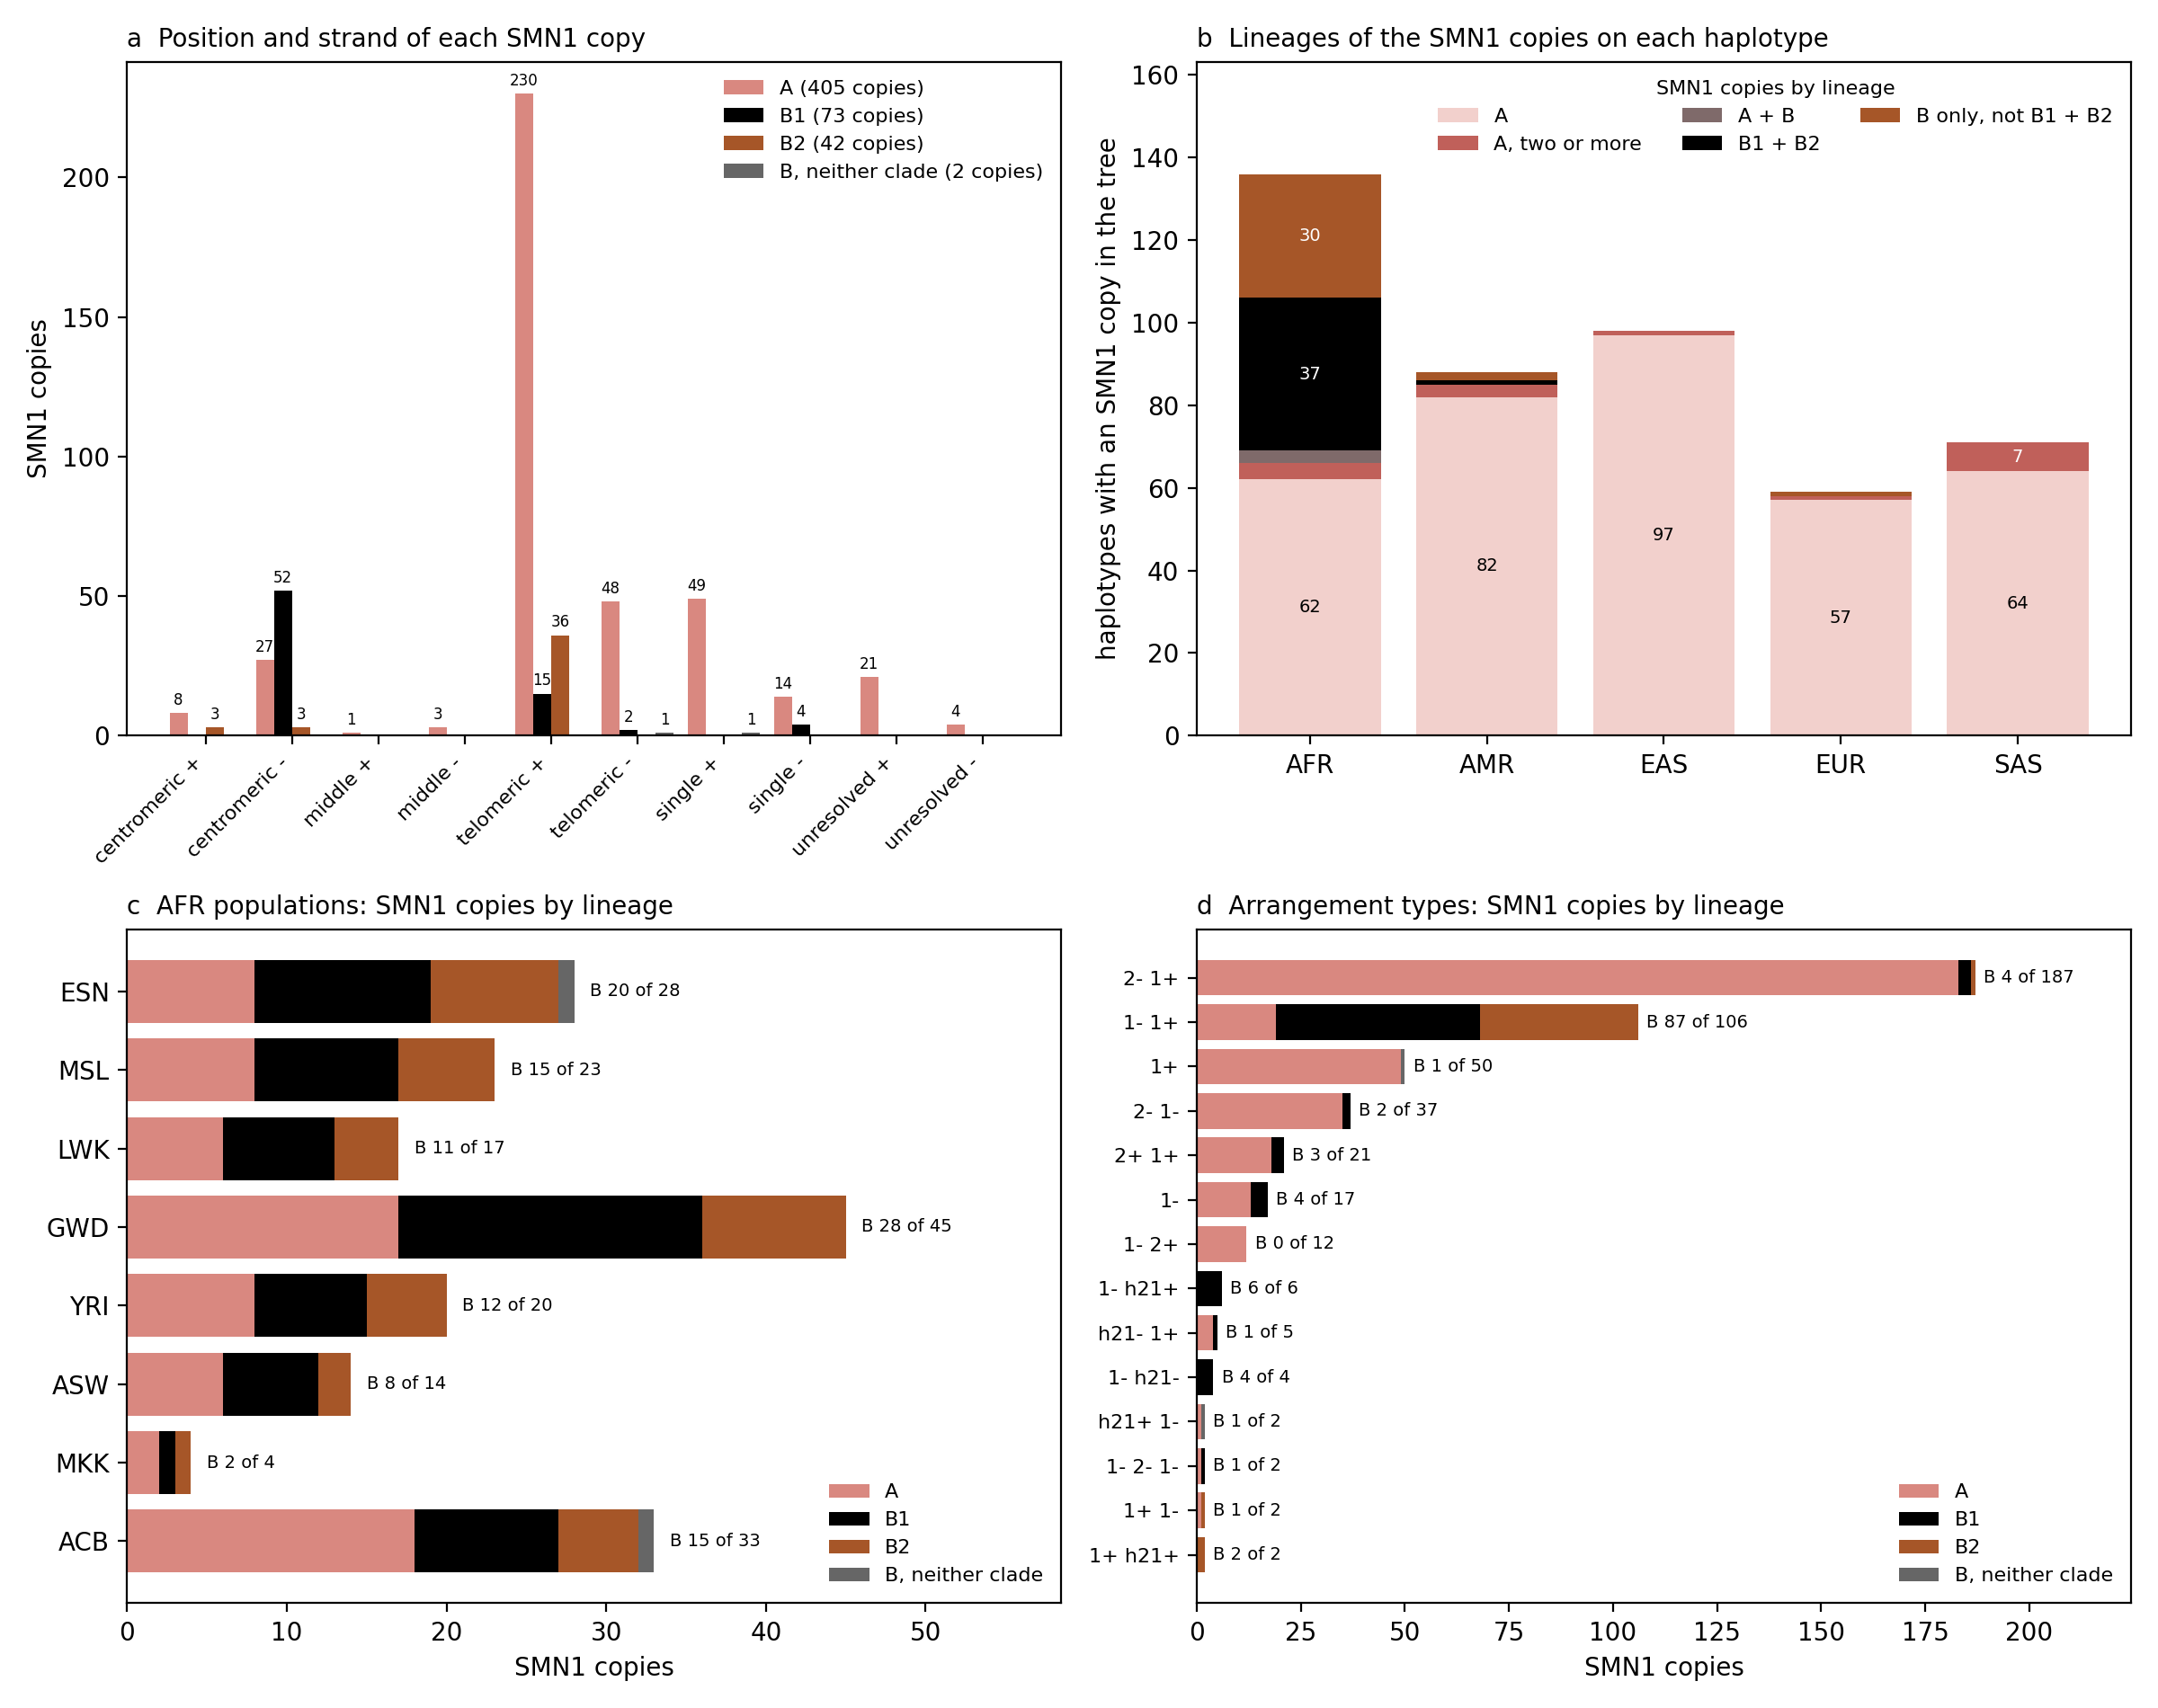
\includegraphics[width=\linewidth]{../figures/lineage_detail.png}
\caption{The two SMN1 lineages, with B split into its sub-lineages (colors as in Figs.~1--5: A red, \linA{} copies; B1 black; B2 brown; B in neither clade gray; \linB{} B copies in all).
\textbf{a}, each copy's copy order among the SMN copies of its haplotype and its strand on GRCh38 (``unresolved'': copy
on an unresolved haplotype, no copy order). \textbf{b}, haplotypes by the lineages of their SMN1 copies, per continental
group (one A copy; two or more A copies; A with a B copy; B1 with B2; one or more B copies, not B1 with B2). \textbf{c}, SMN1 copies by lineage in each African-ancestry population. \textbf{d}, SMN1 copies by lineage in
each arrangement type that holds a B copy or ten or more SMN1 copies. Drawn by \texttt{06\_lineage\_detail.py}.}
\label{fig:lindetail}
\end{figure}

\begin{table}[htbp]\small\centering
\begin{minipage}[t]{0.47\linewidth}\centering
\caption{Haplotypes by the lineages of their SMN1 copies (A; B1, B2; B (n.c.): a B copy in neither sub-clade), per
continental group; ``other'': haplotypes outside the five groups and the reference haplotypes. Written by \texttt{40\_numbers.py} from
\texttt{results/sv/marker\_lineage.tsv}.}\label{tab:lincomp}
{\setlength{\tabcolsep}{3pt}\begin{tabular}{@{}lrrrrrrr@{}}\toprule
& AFR & AMR & EAS & EUR & SAS & other & total\\\midrule
\tabLinComp
\bottomrule\end{tabular}}
\end{minipage}\hfill
\begin{minipage}[t]{0.47\linewidth}\centering
\caption{SMN1 copies by population: all copies, B copies, B as \% of SMN1 copies. The last row pools the AMR, EAS, EUR and SAS populations not listed, and ASL, which has no superpopulation label. The rows hold \ldPopRowsN{} of the \ldPopAllN{} SMN1 copies; the 2 reference copies (GRCh38, CHM13) and the \ldPopNoLabN{} copies of the two donors with no population label (HG005, HG002\_Q100; all lineage A) are not in it. MKK is the Maasai in Kinyawa, Kenya. Written by \texttt{40\_numbers.py}
from \texttt{results/sv/lineage\_population.tsv}.}\label{tab:linpop}
\begin{tabular}{@{}lrrr@{}}\toprule
Population & SMN1 & B & \% B\\\midrule
\tabLinPop
\bottomrule\end{tabular}
\end{minipage}
\end{table}

\subsection{A copy's distance to SMN2 goes mainly with its lineage; where an A copy sits shifts it a little}\label{sec:distctx}
For each SMN1 copy, \texttt{17\_distance\_context.py} takes its mean gene-body distance to the SMN2 copies and compares
it, within each lineage, across where the copy sits (medians, differences per kb; Mann--Whitney or Kruskal--Wallis
tests, descriptive only, since copies are not independent; donor copies only, so the two reference SMN1 copies are
left out). The main text gives these tests by arm (Section~\ref{m:cen}); here they are given by copy order and by whether the copy is on an arm of the palindrome.
\begin{itemize}
\item \textbf{In A, centromeric and telomeric copies are equally far.} Centromeric A copies are \dcACen{} from SMN2
(\dcACenN{} copies) and telomeric ones \dcATel{} (\dcATelN); across centromeric, telomeric and single copies the
distributions differ (Kruskal--Wallis $p=$\,\dcPAPos), from the single copies, which sit slightly further (\dcASingle).
\item \textbf{In A, the palindrome and the arrangement shift it a little.} A copies on an arm of the \RU{A} palindrome
are \dcAPalYes{} from SMN2 (\dcAPalYesN{} copies) and those elsewhere \dcAPalNo{} (\dcAPalNoN; $p=$\,\dcPAPal); across
the arrangement types with ten or more A copies the medians run from \dcAArrMin{} to \dcAArrMax{} ($p=$\,\dcPAArr).
These shifts are clear but small next to the gaps between
lineages (Section~\ref{sec:grpdist}).
\item \textbf{In B, copy order reflects the sub-lineage.} Centromeric B copies are \dcBCen{} (\dcBCenN) and telomeric
ones \dcBTel{} (\dcBTelN; $p=$\,\dcPBPos; within AFR \dcAfrBCen{} against \dcAfrBTel, $p=$\,\dcPAfrBPos). Centromeric B
copies are mostly B1 and telomeric ones mostly B2, and B1 is further from SMN2 than B2 (Section~\ref{sec:grpdist}).
Either way a B copy is further from SMN2 than any group of A copies.
\item \textbf{The palindrome does not set it.} B copies on an arm of the \RU{A} palindrome are \dcBPalYes{}
(\dcBPalYesN{} copies, the \palSmnB{} B copies of Section~\ref{sec:palindrome} and that of \palNoCopyHap, whose \RU{A} pair holds no telSMN copy) from SMN2, those elsewhere \dcBPalNo{} (\dcBPalNoN; $p=$\,\dcPBPal).
\item \textbf{The downstream unit, a hint in B.} B copies in an SMN1-type downstream environment are \dcBEnvOne{} from
SMN2 (\dcBEnvOneN{} copies); in a mixed environment \dcBEnvMixed{} (\dcBEnvMixedN) and in an SMN2-type one \dcBEnvTwo{}
(\dcBEnvTwoN; $p=$\,\dcPBEnv). With so few copies in the last two this is a hint only.
\end{itemize}
\textbf{Speculation (untested).} B1 may have become distant from SMN2 while it sat where it exchanged less sequence with
SMN2 copies. Today's copy positions cannot test this: the distance goes mainly with the lineage and sub-lineage, and where
a copy now sits shifts it by little. A dated tree and the junction sequences between paired copies would be the place to start.

\section{The \RU{A} palindrome: one SMN copy per arm, at mirror positions}\label{sec:palindrome}
Are SMN1 and SMN2 at the center of a palindrome of large repeat units (Fig.~\ref{fig:allhaps})? From the repeat units
\texttt{pangea cohort bundle repeat-units} found (\path{results/decomp/smn.repeat_units.tsv}) and the copies placed in
them, \texttt{13\_palindrome.py} looks for an adjacent inverted pair of \RU{A} units on each of the \palHaps{}
resolved haplotypes with repeat units (the other \palNoUnits{} resolved haplotypes, each with one SMN copy, have no
recurring bundle apart from the tandem-array bundle and so no unit; GRCh38, kept by the step as a reference row, is not counted).
\begin{itemize}
\item \textbf{The core is a near-symmetric palindrome.} \palAdj{} haplotypes carry an adjacent inverted \RU{A} pair:
\palHead{} head to head (\RU{A}+ \RU{A}$-$) and \palTail{} tail to tail (\RU{A}$-$ \RU{A}+; \palTailHaps, arrangements \palTailArr, each
with at most one SMN copy on either side). Of the head-to-head pairs, \palPair{} carry an SMN copy on each arm; the other
(\palNoCopyHap) has none on its telomeric arm. Those \palPair{} are the palindrome of this section, and every arm
length and copy distance is measured from their \RU{A}+ \RU{A}$-$ junction. The two \RU{A} units are a median \palArmL{} and
\palArmR{} kb long (median difference \palArmDiff{} kb), separated by a median \palGap-kb stretch no unit covers (the short one of the two clusters of Section~\ref{m:arr} is nearly always on a haplotype whose cenSMN arm carries X, \palGapShortCOne{} of \palGapShortN{} C1 against \palGapLongCOne{} of \palGapLongN{} for the long one, Fisher $p=$\,\palGapTypeP, as where a unit ends is set by what follows the core; Section~\ref{m:arms}); the axis S
lies next to it inside one of the \RU{A} units, and inside no unit of another family, on \palSinA{} of the \palGapSN{} copies of S at the axis (on \palGapSHaps{} haplotypes).
They include \palTwoOne{} ``2-~1+'' and \palOneOne{} ``1-~1+'' haplotypes.
\item \textbf{The SMN copies sit on the arms, at mirror positions, not at the center.} Every one of the \palPair{}
haplotypes has an SMN copy on each arm (\palCopies{} items, one counted copy per arm plus one truncated piece, so \palThreeCopy{} haplotype has three items). They lie
\palDmin--\palDmax{} kb from the axis (median \palDmed{} kb); the nearest copies on the two arms differ in their
distance from the axis by a median \palMirror{} kb. Inside its own \RU{A} unit a copy sits \palRelMin--\palRelMax\% of the
way from the unit's 5\(^\prime\) end (median \palRelMed\%; \palInUnit{} copies inside one \RU{A} unit), close to that end.
This is why paired copies lie about twice \palDmed{} kb apart. The truncated piece is on \palThreeHap.
\item \textbf{Beyond the core the units seldom mirror.} Of the \palRoom{} pair haplotypes with at least one more
unit on both sides, \palDeeper{} mirror one further pair (\palDeeperHap). The palindrome is the \RU{A} pair itself, not the whole region.
\item \textbf{What flanks the pair.} Family letters are those of Section~\ref{sec:compared}; families with fewer than ten occurrences are not in Table~\ref{tab:unitfam}. On the \palFlankN{} pairs, the unit next to \RU{A}+ on the centromeric side is
\palFlankLText; the unit next to \RU{A}$-$ on the telomeric side is \palFlankRText. An \RU{B} unit (mostly Xi$'$ and Xi,
Table~\ref{tab:unitfamel}) lies on both sides, \RU{B}$-$ before the pair and \RU{B}+ after it (often beyond an \RU{D}$-$ or \RU{E}+ unit), on
\palFlankBB{} haplotypes. These \RU{B} units face opposite ways but are not adjacent to the pair on both sides, so they are
not counted as a mirrored unit pair above.
\item The other \palNoPair{} haplotypes have no such palindrome (\palNoAdj{} have no adjacent inverted \RU{A} pair; among them \palNoOne{} ``1+'',
\palNoTwoMOneM{} ``2-~1-'' and \palNoTwoPOneP{} ``2+~1+'').
\end{itemize}

The units are what PANGEA found to recur within each haplotype; their ends, and so the axis, are known only to the
resolution of its bundles.
Fig.~\ref{fig:palindrome} draws this: what each arm holds in AFR haplotypes and in the other groups, the four
forms of the palindrome, every pair haplotype aligned on its axis and colored by element, and the nearest copy on each
arm against the other; one haplotype of each of the two commonest forms is drawn to scale with its genes in
Fig.~\ref{fig:locus}.

\paragraph{The arms as named elements (Table~\ref{tab:elements}).} \texttt{28b\_arm\_elements.py} puts every bundle
segment of each pair haplotype's window on the cenSMN arm (left of the axis) or the telSMN arm (right) by its midpoint,
measures it in kb from the axis, and reads it outward: its token is the bundle id with its strand as seen walking away
from the axis. Tokens are named by the sets of Table~\ref{tab:elements}, the bundles that
come and go together beyond the core. The core is the arm from the axis to the outer end of the first
end-of-core run beyond \elAstart~kb (a median \elAEnd~kb), whatever lies inside; the layout of an arm is the series of named
elements beyond the core, with runs collapsed and other bundles skipped. Pieces of one element are joined across bundle-free
gaps, which is how step 28b's element Xi spans its tandem array. The text names its two parts Xi$'$ (bundles 1 and 5, nearer the core) and Xi (the rest); every block holds bundles of one part only (\xpBlocks{} blocks, checked), and Figs.~\ref{fig:locus}, \ref{fig:palindrome} and~\ref{fig:dotplots} label blocks by part and color Xi$'$ paler than Xi.
\begin{itemize}
\item \textbf{X.} X is Xi (bundles 13 16 17 21 24 3, inverted), S and Xd, the same bundles direct: an inverted repeat centered on S. Xi$'$ (bundles 1 and 5, inverted) is not part of it; it is separated from Xi by the tandem array, and the two together hold all the core's bundles. They are parts of one inverted copy of the core, so neither is the older; the prime marks only the part outside X. On the \xSpanN{} C1 arms with the commonest layout X is of one of two lengths: \xFormShortKb~kb on \xFormShortN{} arms and \xFormLongKb~kb on \xFormLongN, with no arm in between (\xFormBigN{} arms are longer, \xFormBigKb~kb: \xFormBigHaps). The two forms carry the same bundles in the same order and differ in how much of bundle 3, which lies on either side of S, each side holds: on the Xd side a median \xFormShortBd~kb in the short form against \xFormLongBd{} in the long one (on the Xi side \xFormShortBi{} against \xFormLongBi). The short form goes with a telSMN arm that carries X as well: \xFormShortTOne{} of the \xFormShortN{} short arms are on a T1 haplotype, against \xFormLongTOne{} of the \xFormLongN{} long (Fisher $p=$\,\xFormP). The stretch from Xi$'$'s start to Xd's end is \xFullLo--\xFullHi~kb. Xi$'$ (median \xInMed~kb) and the tandem array between it and Xi (median \xGapMed~kb) carry nearly all of that spread.
\item \textbf{Types by Xd.} Wherever Xd occurs it covers at least \elXdMin~kb of bundles, so no arm sits near the cut.
On every cenSMN arm, the inverted core copy (Xi$'$ or Xi) and Xd occur together or not at all (checked; \xpCOneBoth{} of the C1 arms carry both Xi$'$ and Xi): \elCOne{} arms are C1 and \elCZero{} are C0.
On the telSMN arm every arm carries Xi and S (Xi$'$ on all but \xpTelNoPrime); \elTZero{} are T0 (no Xd) and \elTOne{} T1. The \xcNoS{} C1 arms with no S between Xi and Xd are \xcNoSNames; the window of the first holds a \gapNoSKb-kb assembly gap.
\item \textbf{Commonest layouts.} C1: core, Xi$'$, Xi, S, Xd, end of the core, E, flank (\elCOneCan{} of \elCOne); C0: core, E, flank
(\elCZeroCan{} of \elCZero); T0: core, E, end of the core, Xi$'$, Xi, S (\elTZeroCan{} of \elTZero); T1: core, E, Xi, S, Xd, end of the
core, E, flank, end of the core, Xi$'$, Xi, S (\elTOneCan{} of \elTOne). The other arms of each type carry an extra element or
lack one (E on \elEtel{} of \elHaps{} telSMN arms; on all \elEcen{} cenSMN arms); their layouts are listed in
\path{results/sv/arm_elements.tsv}.
\item \textbf{Where the elements lie} (median block ends on arms with the commonest layout, kb from the axis). C1: Xi
\elCXiLo--\elCXiHi, S \elCSLo--\elCSHi, Xd \elCXdLo--\elCXdHi, E \elCELo--\elCEHi; C0: E \elZELo--\elZEHi; T0: Xi
\elTXiLo--\elTXiHi.
\item \textbf{The forms.} C1|T0 \elFonezero{} haplotypes (\elFonezeroAfr{} AFR), C1|T1 \elFoneone{} (\elFoneoneAfr),
C0|T0 \elFzerozero{} (\elFzerozeroAfr), C0|T1 \elFzeroone{} (\elFzerooneAfr). T1 arms: \elTOneAfr{} of \elAfrHaps{} AFR
haplotypes, \elTOneEas{} EAS.
\end{itemize}

\begin{table}[htbp]\small\centering
\caption{The arm elements: the bundle tokens (bundle id of the study's decomposition, \texttt{results/decomp/smn.bed},
with its strand read outward from the axis) that name each element. Written by \texttt{28b\_arm\_elements.py}
(\texttt{results/sv/arm\_element\_sets.tsv}).}\label{tab:elements}
\begin{tabular}{@{}>{\raggedright}p{4.2cm}>{\raggedright\arraybackslash}p{10.5cm}@{}}\toprule
Element & Bundle tokens\\\midrule
\tabElements
\bottomrule\end{tabular}
\end{table}

\paragraph{The \RU{A} unit and the elements.} At the study's bundle scale the \RU{A} unit ends near the end of the core: short of it where the cenSMN arm goes on with X (C1|T0, both arms on \auCOTZeroNeither{} of \auCOTZeroN{} haplotypes) and beyond it, over the core's end and E, where both arms go on with them (C0, both arms on \auCZeroBoth{} of \auCZeroHaps); on C1|T1 haplotypes only the telSMN unit runs past (\auCOTOneTelOnly{} of \auCOTOneN; Section~\ref{m:arms}, step 28j, \path{results/sv/a_unit_length.tsv}). It reaches \elUnitLong~kb or more on \elCOneLong{} of the \elCOne{} C1, \elCZeroLong{} of the
\elCZero{} C0, \elTZeroLong{} of the \elTZero{} T0 and \elTOneLong{} of the \elTOne{} T1 arms. With finer bundles the
same program took X into the \RU{A} unit on some arms and not others, for a reason that has to do with the arms' tandem
arrays and not with their content (Section~\ref{sec:fine}); the elements are read the same way at either scale. On the \auHaps{} pair haplotypes the core reaches a median \auCore~kb from the axis (10th--90th percentile \auCoreLo--\auCoreHi~kb). What follows the core sets where the unit ends: E follows directly on every C0 cenSMN arm (\auCZeroCenE{} of \auCZeroCenN) and on \auTelE{} of the \auHaps{} telSMN arms (E is on \elEtel{} of them; on \auTelENotNext{} it lies further out), while Xi$'$ follows the core's end on \auCOneCenXi{} of the \auCOneCenN{} C1 cenSMN arms. Median unit lengths are \auCZeroUnit~kb on C0 haplotypes (\auCZeroOver~kb beyond the core), \auCOTZeroUnit~kb on C1|T0 (\auCOTZeroShort~kb short of it), and \auCOTOneTelUnit{} against \auCOTOneCenUnit~kb on C1|T1.

\paragraph{X splits NAIP.} \texttt{28b\_arm\_elements.py} places every \emph{NAIP} match of the window
(\path{results/copies/features.tsv}) on its arm by its span (\path{results/sv/arm_naip_pieces.tsv}). A whole
\emph{NAIP} crosses the end of the core on all \elNaipWholeCZero{} C0 arms, on \elNaipWholeTZero{} of \elTZero{} T0 and
\elNaipWholeTOne{} of \elTOne{} T1 arms, and ends a median \elNaipPast~kb beyond it. On \elNaipSplit{} of the
\elCOne{} C1 arms its 3$^\prime$ part (transcript bases \elNaipStartA{} or \elNaipStartB{} onward, on \elNaipFromA{} and
\elNaipFromB{} arms) ends at the end of the core and Xi$'$ begins a median \elNaipGapA{} or \elNaipGapB~kb further out;
the gene's first \elNaipTxB{} bases lie beyond X on all \elNaipFive{} C1 arms; on \elNaipWholeCOne{} C1 arms a whole gene crosses the end of the core instead. On \elNaipTZeroThree{} of the \elTZero{} T0 arms (and \elNaipTOneThree{} of the \elTOne{} T1 arms) a
3$^\prime$ part sits on the copy of the core's end just before Xi$'$: the junction of the core's end and Xi$'$ falls at the
same point of \emph{NAIP} wherever Xi$'$ follows the core's end. \texttt{28f\_naip\_exons.py} places the pieces' ends on the RefSeq transcript \nxTx{} (\nxExons{} exons)
(\path{data/refs_seq/naip_refseq_nm.gb}, fetched from NCBI): its first 31 bases map to the window position where the gene
features put the start of GRCh38's \emph{NAIP}, and every piece end in \path{arm_naip_pieces.tsv} is an exon junction of it
or the transcript end the gene features use (\path{results/sv/naip_exons.json}). The 3$^\prime$ part starts at exon
\nxThreeAExon{} (codon \nxThreeACodon) or exon \nxThreeBExon{} (codon \nxThreeBCodon); the 5$^\prime$ part runs from exon 1
to exon \nxFiveExon{} (codons 1--\nxFiveCodon{} of \nxCodons), holding the protein's BIR1 and BIR2 domains whole and the start of BIR3;
the 3$^\prime$ part from exon \nxThreeAExon{} holds BIR3 whole, the one from exon \nxThreeBExon{} only the last bases of BIR3. Exons
\nxThreeAExon--\nxFiveExon{} (\elNaipOverlap{} transcript bases) are in both parts where the 3$^\prime$ part starts at exon \nxThreeAExon.
Whether either part is transcribed was not examined.

\paragraph{S by sequence.} \texttt{28c\_spacer\_sequence.py} cuts each of the \sOcc{} S occurrences (median
\sLen~kb) from its window. Its orientation by \sK-mer containment of a reference S agrees with the strand of its
bundle on all \sOrientAgree, so the orientation flips the bundle shows are real. Aligned end to end (edlib \verEdlib) to
the same haplotype's axis S, the S of X on the cenSMN arm is close (\sCenSa{} of \sCenAll; median \sSaMed{}
differences per kb) and the S on the telSMN arm is not (\sTelSt{} of \sTelAll; median \sStMed{} per kb; the other \sTelUntyped{} of the \sTelOcc{} telSMN S, both on \sNoAxisHap, have no S at the axis to compare with); no distance
falls between \sGapLo{} and \sGapHi{} per kb, and the variants are split at \sCut. Between haplotypes, axis S copies differ by a median
\sAxisBetween{} and telSMN S copies by \sTelBetween{} per kb (\sSample{} haplotypes sampled). S sits at the main axis once on \elAxisS{} of the \elHaps{} haplotypes, twice on \sAxisTwo{} (\sAxisTwoHaps) and not at all on \sAxisNoneHaps, whose window holds a \gapNoAxisKb-kb assembly gap; at the axis \sAxisFwd{} copies lie in one orientation and \sAxisRev{} in the other. S is on the cenSMN arm of \sCenHaps{} of the \elCOne{} C1 haplotypes, once on \sCenOnce{} and more than once on \sCenMore; a T0 arm carries one S (\sTelTzeroN{} copies) and a T1 arm two, three on \sTelToneThree{} of the \sTelToneArms{} (\sTelToneN{} copies).

\paragraph{Tandem arrays.} PANGEA's \texttt{tandem-repeats} over every window (step 28) finds $\sim$20-kb arrays at
three places on the arms (\path{results/sv/arm_element_arrays.tsv}): inside the core, of \elInnerUnit-kb units; between Xi$'$ and Xi
on the cenSMN arm of C1 haplotypes (\elOutCOne{} of \elCOne{} arms; \elOutCZero{} of the C0 arms), of
\elOutCUnit-kb units, a median \elOutCCopies{} units; and between Xi$'$ and Xi on the telSMN arm, of \elOutTUnit-kb units, a
median \elOutTZeroCopies{} units on T0 (\elOutTZero{} arms) and \elOutTOneCopies{} on T1 (\elOutTOne{}; Mann--Whitney
$p=$\,\elOutTP). The copy's distance from the axis rises with the inner array (Spearman \elRhotel{} on the telSMN arm,
\elNInnertel{} arms with the array; \elRhocen{} on the cenSMN arm); the copy lies a median \elCopyAtInnerTwo, \elCopyAtInnerThree{} and \elCopyAtInnerFour~kb from the axis with two, three and four units on the telSMN arm.

\paragraph{Why the copy sits further out on C0 and T1 arms.} \texttt{28g\_copy\_position.py} splits each arm's
axis-to-copy distance into the stretch of the core covered by the inner array's bundle and the rest
(\path{results/sv/copy_position.tsv}). The copy sits \cpDiffCopycen~kb further out on C0 than on C1 arms (medians
\cpCopyCZero{} and \cpCopyCOne~kb) and \cpDiffCopytel~kb further on T1 than on T0 arms (\cpCopyTOne{} and
\cpCopyTZero~kb). At this bundle scale the array's bundle covers only part of the array, so the stretch it spans
(\cpArrCZero{} against \cpArrCOne~kb on C0 and C1 arms) does not account for the whole difference: the rest differs
too (\cpRestCZero{} against \cpRestCOne~kb). With the finer bundles the split was clean (Section~\ref{sec:fine}).

\paragraph{The palindrome in the sequence itself (Fig.~\ref{fig:dotplots}).} A dot plot of a window against itself shows
the pair without the repeat-unit calls: each dot is a shimmer (sparse minimizer pair; $w=\dpW$, $k=\dpK$, $r=\dpR$)
shared by two places in the window; a forward repeat runs parallel to the main diagonal and an inverted repeat across
it. One haplotype of each form is drawn; a and d are those of Fig.~\ref{fig:locus}. The \RU{A}+ \RU{A}$-$ pair is a line across
the diagonal through the axis on all four, with an SMN copy on each side of it. X shows in the sequence: on the cenSMN
arm beyond the core, the C1 haplotypes have \dpACen{} and \dpBCen{} dots with both ends there, the C0 haplotypes \dpCCen{} and
\dpDCen.

\begin{figure}[htbp]\centering
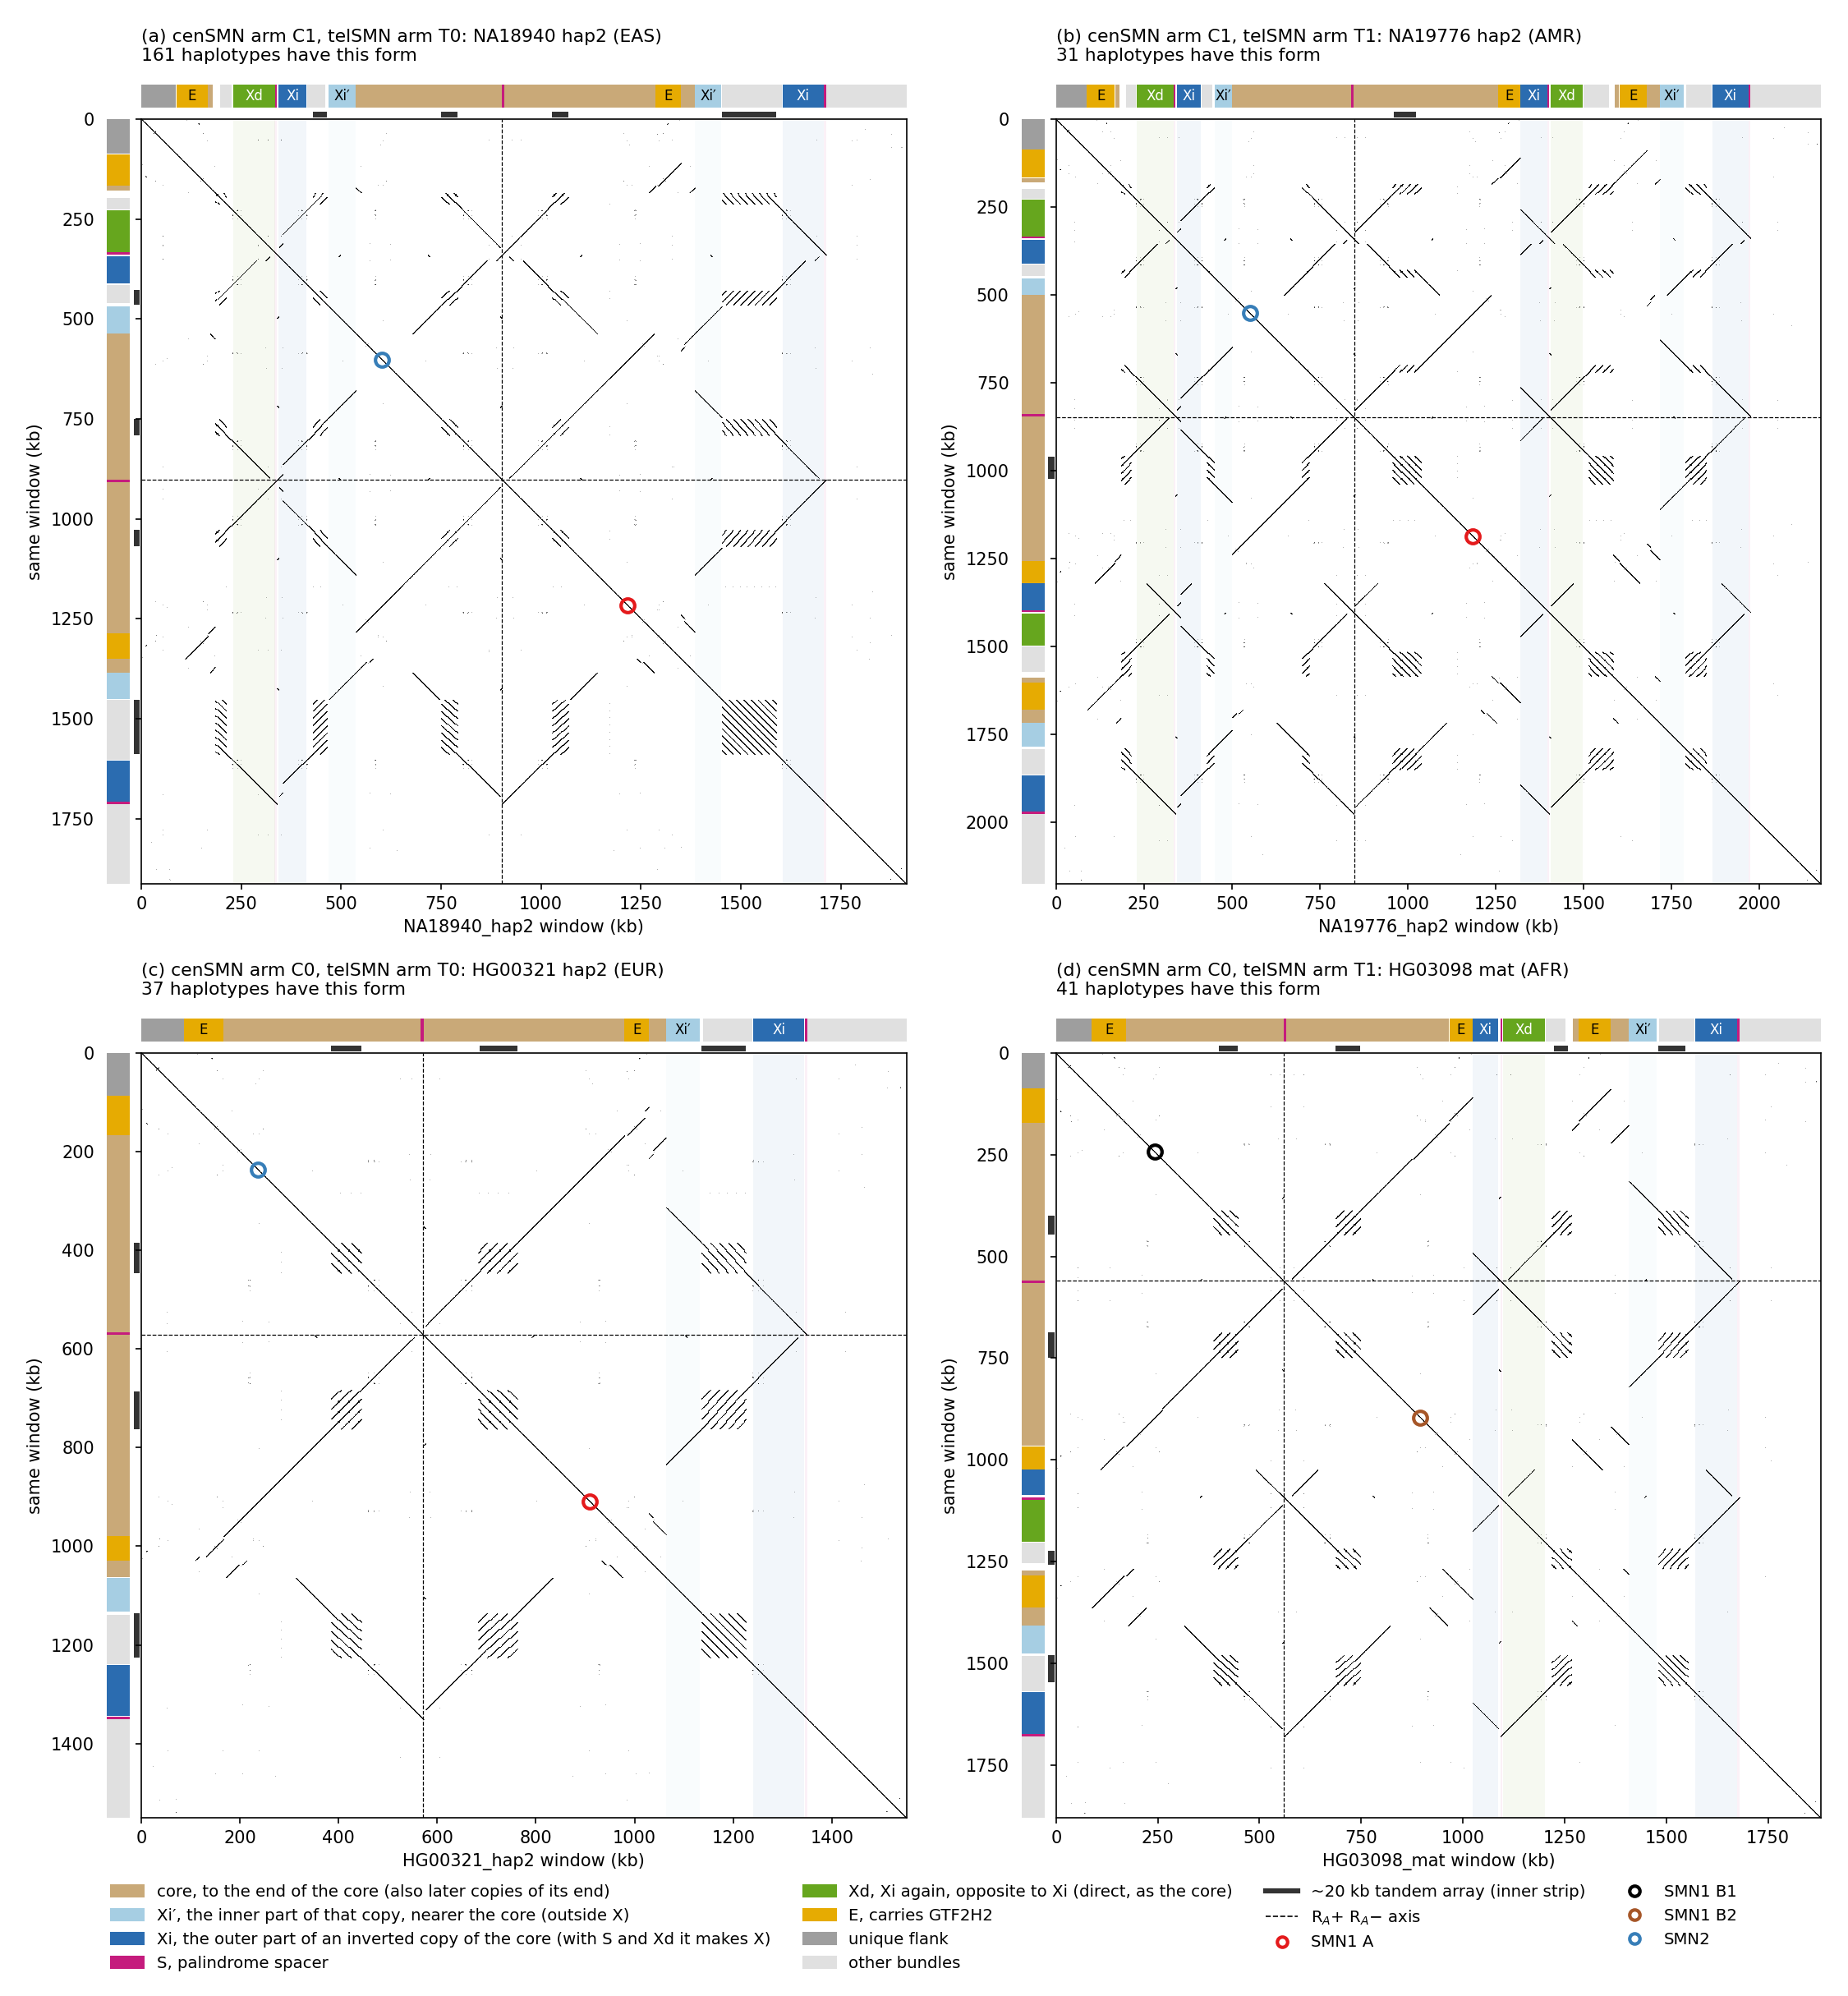
\includegraphics[width=\linewidth]{../figures/self_dotplots.png}
\caption{Self dot plots of one haplotype of each form: \textbf{a}, \dpAName{} (C1|T0; window \dpALen{} kb),
\textbf{b}, \dpBName{} (C1|T1; \dpBLen{} kb), \textbf{c}, \dpCName{} (C0|T0; \dpCLen{} kb) and \textbf{d},
\dpDName{} (C0|T1; \dpDLen{} kb). Dots: shimmers shared by two positions of the window (PANGEA's shimmer matcher, \texttt{get\_shmmr\_dots},
$w=\dpW$, $k=\dpK$, $r=\dpR$, minimum span \dpSpan). Strips along the axes: the arm elements (colors as in
Fig.~\ref{fig:palindrome}), S also at the axis, and the $\sim$20-kb tandem arrays (thin inner strip); shading marks Xi$'$, Xi,
S and Xd across the plot. Dashed lines: the axis of the \RU{A}+ \RU{A}$-$ pair. Circles: the SMN copies, on the main diagonal,
colored by gene and lineage. Drawn by \texttt{scripts/34\_dotplots\_graph.py}.}\label{fig:dotplots}
\end{figure}

\paragraph{Why X is called X (Fig.~\ref{fig:xcross}).} Drawn against itself, the cenSMN arm of a C1 haplotype shows
X directly: beyond the core, Xi and Xd form an inverted repeat, whose dots run across the main diagonal and
cross it at S (about \xcExS~kb from the axis in HG01099 mat). The element thus draws an X, and S, its center, is part of
it; the short break in the cross at S is the spacer itself, which has no partner. The C0 arm of the same donor has no
cross. Over all palindrome haplotypes, on each cenSMN arm \xcLo--\xcHi~kb from the axis we found where the off-diagonal
dots are centered (an inverted repeat centered at $c$ puts its dots on $x+y=2c$): on \xcTwenty{} of the \xcCOneS{} C1 arms
with an S in that stretch the strongest center lies within 20~kb of S, on \xcTen{} within 10~kb. The other \xcNoS{} C1 arms (\xcNoSNames) carry Xi and Xd with no S between
them and were not scored.

\begin{figure}[htbp]\centering
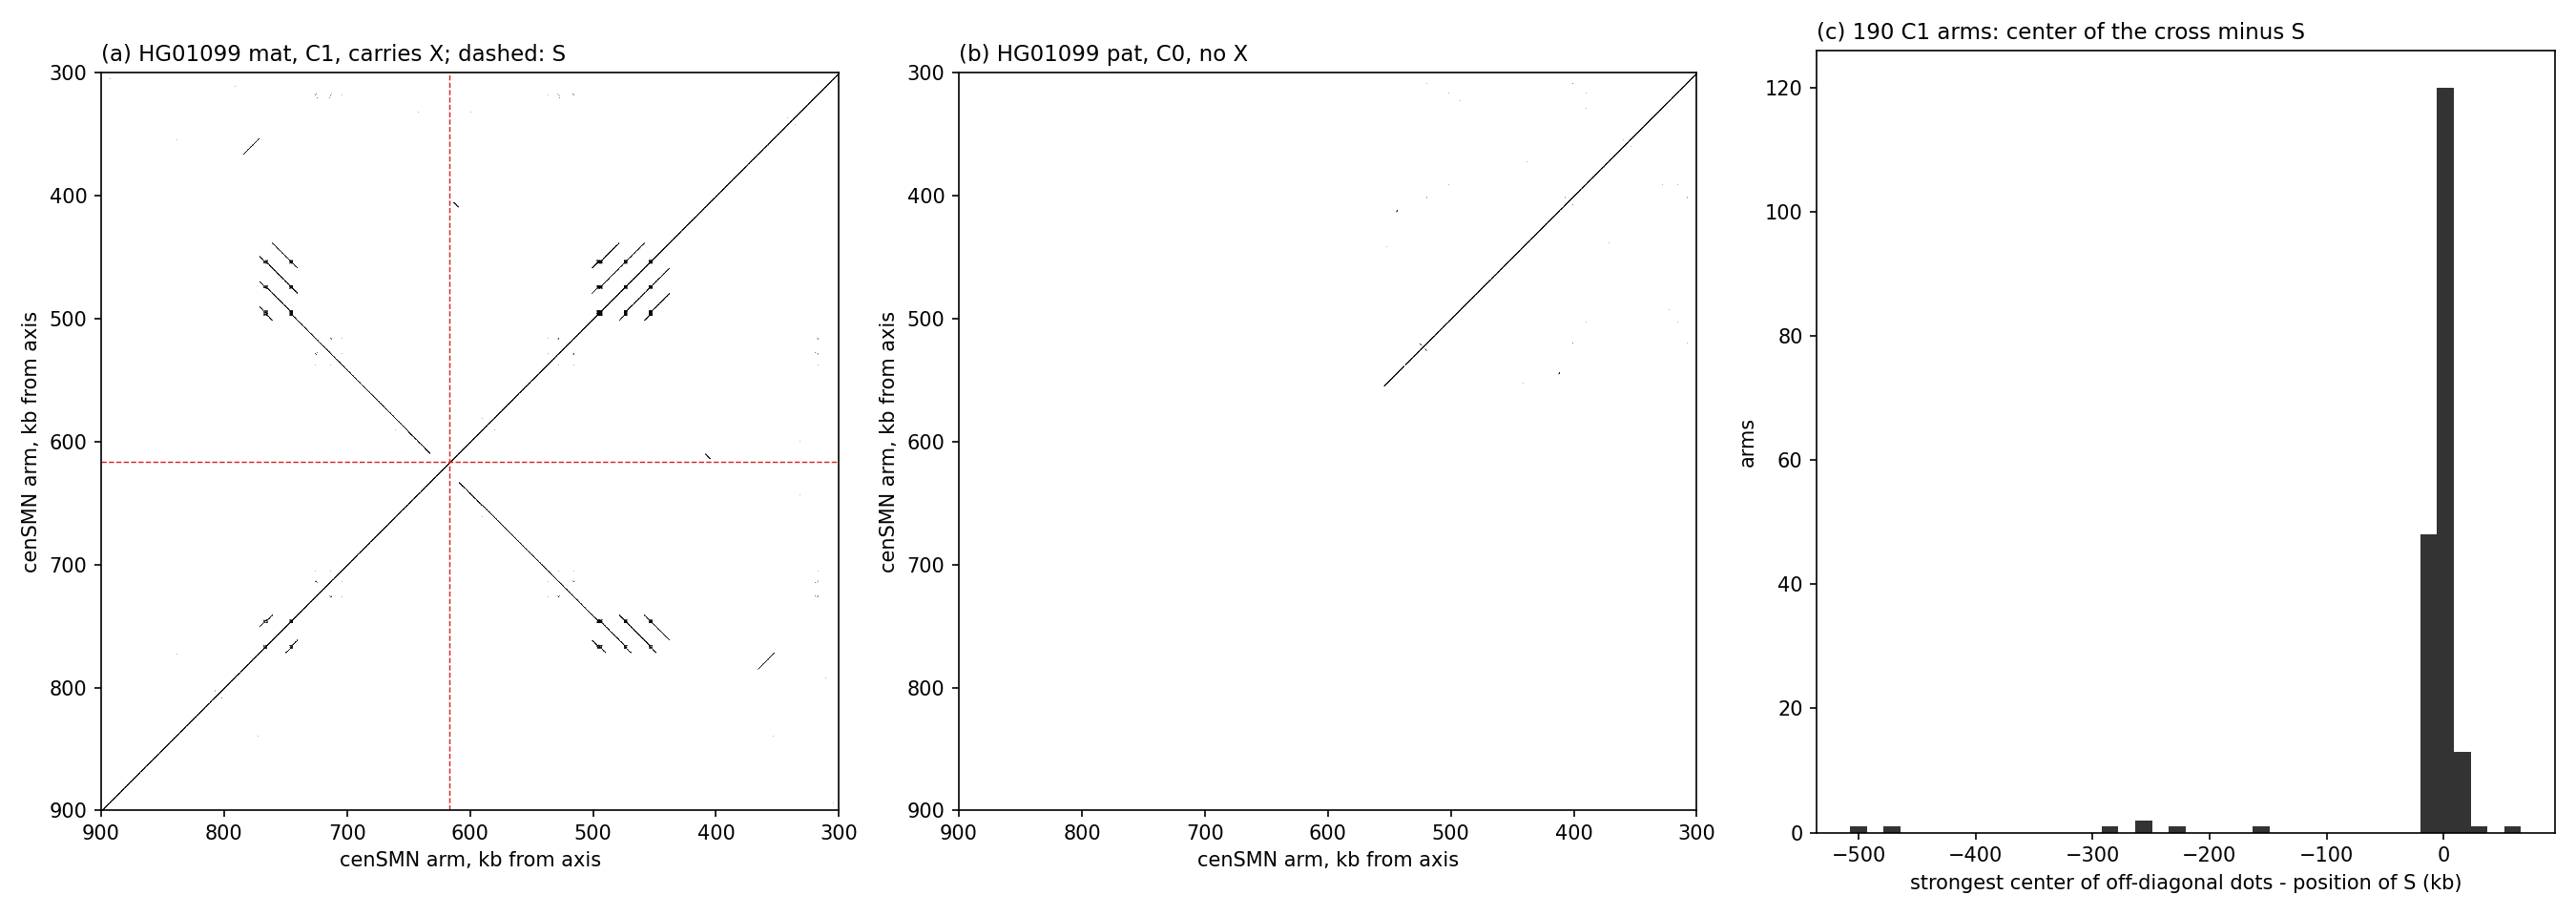
\includegraphics[width=\linewidth]{../figures/x_cross.png}
\caption{X in the sequence. \textbf{a}, \textbf{b}: self dot plots of the cenSMN arm, \xcLo--\xcHi~kb from the axis
(shimmers as Fig.~\ref{fig:dotplots}), of the two haplotypes of donor HG01099: \textbf{a}, mat, C1, whose X draws a
cross centered on S (dashed lines); \textbf{b}, pat, C0, no cross (its window ends \xcExCZeroArm~kb from the axis).
\textbf{c}: on the \xcCOneS{} C1 arms with an S in that stretch, the strongest center of the off-diagonal dots minus the
position of S. Drawn by \texttt{scripts/38\_x\_cross.py}.}\label{fig:xcross}
\end{figure}

\paragraph{SMN1 lineages on the arms.} Coloring the SMN1 copies of Fig.~\ref{fig:palindrome}c by lineage
(Section~\ref{sec:posstrand}) shows the same split as the copy positions. Of the \palSmnA{} lineage-A SMN1 copies on
the pair, \palARight{} sit on the right (\RU{A}$-$, telomeric) arm and \palALeft{} on the left. Of the \palSmnB{} lineage-B
copies, B1 sits on the left (\RU{A}+, centromeric) arm (\palBoneLeft, against \palBoneRight{} on the right) and B2 on the
right (\palBtwoRight, against \palBtwoLeft). The \elBB{} haplotypes with one B1 and one B2 copy all fall in the C0 forms
of panel c (\elBBTOne{} of them C0|T1). B copies sit somewhat further from the axis than A copies
(median \palBDist{} against \palADist{} kb; Mann--Whitney $p$~=~\palPDist{}), and the mirror is no less exact on
B-carrying haplotypes (median difference \palBMirror{} against \palOthMirror{} kb). These are descriptive: copies on one
haplotype are not independent, and B is almost only African.

\paragraph{Which copy sits on each arm (Table~\ref{tab:slots}).} Lefebvre et al.~\cite{lefebvre1995} named the two
SMN loci by position: telSMN, the telomeric copy (usually SMN1), and cenSMN, the centromeric copy (usually SMN2). On the
pair, the copy on the right (\RU{A}$-$, telomeric) arm is at the telSMN position and the copy on the left (\RU{A}+, centromeric) arm
at the cenSMN position. The right arm holds an SMN1 of lineage A in \slROthA{} of the \slROth{} haplotypes outside AFR. The left arm differs between the groups. Outside AFR it holds SMN2 in \slLOthTwo{} of
\slLOth{} (lineage A \slLOthA, lineage B \slLOthB). In AFR haplotypes it holds lineage B in \slLAfrB{} of \slLAfr{} (B1 \slLAfrBone, B2 \slLAfrBtwo),
SMN2 in \slLAfrTwo{} and lineage A in \slLAfrA: in this cohort's AFR haplotypes the commonest gene at the cenSMN
position is an SMN1 of sub-lineage B1. At the telSMN position of AFR haplotypes, B2 (\slRAfrBtwo) and A (\slRAfrA) are
about equally common, and B1 is rarer (\slRAfrBone).

This says where the copies sit today, not how they came to be there. Gene conversion
between the two loci is documented: van der Steege et al.~\cite{vandersteege1996} found hybrid genes of both kinds,
and Campbell et al.~\cite{campbell1997} report SMN1 replaced by its centromeric counterpart in milder SMA, the
opposite direction to B1. A conversion that turned a cenSMN copy into B1 would have
had to span the whole gene body, since B1 differs from SMN2 throughout it (Section~\ref{sec:grpdist}); these data do
not decide how B1 came to sit there.

\begin{table}[htbp]\small\centering
\caption{The copies and pieces on each arm of the \palPair{} pair haplotypes, by class (SMN1 split by lineage), for
AFR haplotypes and all others (``other'' includes the few ASL and unlabeled haplotypes). Column ``other'': the seven
$\Delta$7--8 copies and the one truncated piece, which shares its left arm with a counted copy (NA18959 hap1), so the
left arms hold one item more than the right (\slLOthItems{} items on the \slLOth{} left arms of the other groups). Hybrid: h12 and h21. Items: copies and pieces, not arms. From \texttt{27\_arm\_contents.py}
(\texttt{results/sv/arm\_slots.tsv}).}\label{tab:slots}
\begin{tabular}{@{}llrrrrrr@{}}\toprule
Arm & Haplotypes & SMN2 & SMN1 A & SMN1 B & Hybrid & Other & Items\\\midrule
\tabSlots
\bottomrule\end{tabular}
\end{table}

\paragraph{An arm holds one SMN copy.} \texttt{27\_arm\_contents.py} takes each of the \armN{} arms of the pair
haplotypes on its own. Every arm holds exactly one counted SMN copy (\armOneCopy{} of \armN; one left arm, NA18959 hap1,
also holds a truncated piece), inside the core on every arm (checked in step 28b); no element beyond the core holds an SMN copy.

% figure fig:palindrome is in the main text


\section{The structure differs between continental groups, most between AFR and the rest (Fig.~\ref{fig:ancestry})}\label{sec:ancestry}
\textbf{Question.} Does the large-scale structure of the region differ between the five continental groups? Unit: the
\anHaps{} resolved haplotypes of \anPeople{} people in AFR (\anNAfr), AMR (\anNAmr), EAS (\anNEas), EUR (\anNEur) and
SAS (\anNSas); ASL and unlabeled samples are left out. Every test permutes the group label of whole people (both
haplotypes together), so a person's two haplotypes are not counted as independent. Drawn and computed by
\texttt{09\_ancestry\_structure.py}.

\textbf{Answer: yes, and most of the difference is AFR against the rest, but not all of it.}
\begin{itemize}
\item \textbf{Arrangement types} (\anTypes{} types on five or more haplotypes, \anRare{} haplotypes of rarer types
pooled): $\chi^2=\anChi$, Cram\'er's $V=\anV$, permutation $p\le\anPArr$ (the floor that \anPerm{} permutations allow).
``2-~1+'' is \shTwoMOnePAfr\% of AFR haplotypes against \shTwoMOnePEur--\shTwoMOnePEas\% elsewhere (\shTwoMOnePEur\%
EUR, \shTwoMOnePSas\% SAS, \shTwoMOnePAmr\% AMR, \shTwoMOnePEas\% EAS); ``1-~1+'' is \shOneMOnePAfr\% in AFR against
at most \shOneMOnePSas\%; ``2+~1+'' (the GRCh38 type) is commonest in EAS (\shTwoPOnePEas\%); the $\Delta$7--8
type ``d2-~1+'' is seen only in AMR (\shDelTwoAmr\%) and EUR (\shDelTwoEur\%).
\item \textbf{Structural distance} (PANGEA's bundle distance): PERMANOVA over the five groups pseudo-$F=\anFAll$,
$R^2=\anRsqAll\%$, $p\le\anPAll$; over the four groups other than AFR, pseudo-$F=\anFNonAfr$, $R^2=\anRsqNonAfr\%$,
$p=\anPNonAfr$ (\anPermPA{} permutations each). Groups differ, but group explains under a tenth of the variation.
Median distance within a group is lowest in EAS (\anWEas) and highest in AFR (\anWAfr) and EUR (\anWEur), and AFR
haplotypes are about as far from each other as from any other group (between-group medians from \anAfrBetweenMin).
\item \textbf{Counts per haplotype} (group means; Kruskal--Wallis, people permuted):
the number of SMN copies per haplotype does \emph{not} differ (\anSmnAfr{} AFR to \anSmnAmr{} AMR, $p=\anPSmn$;
SERF1 $p=\anPSerf$), but what the units hold does: SMN1 by exon 7 is \anOneAfr{} in AFR against
\anOneEas--\anOneSas{} elsewhere, SMN2 \anTwoAfr{} in AFR against \anTwoEas{} in EAS ($p\le\anPOne$ and \anPTwo);
full-length NAIP follows SMN1 (\anNaipAfr{} AFR, \anNaipAmr--\anNaipEas{} elsewhere, $p=\anPNaip$); GTF2H2
(\anGtfEas{} EAS to \anGtfEur{} EUR, $p=\anPGtf$) and large repeat units (\anUnitsEas{} EAS to \anUnitsEur{} EUR,
$p=\anPUnits$) are lowest in EAS.
\end{itemize}
Read together: AFR haplotypes more often carry SMN1 where others carry SMN2 (the ``1-~1+'' type, B1 and B2 above) and are the
most varied; EAS haplotypes are the most alike; and the non-AFR groups also differ among themselves, though less.
The structural distance is PANGEA's score on the top bundles of each window, not the study's arrangement strings, and
the 1000 Genomes continental groups are coarse labels for the populations sampled.

\begin{figure}[htbp]
\centering
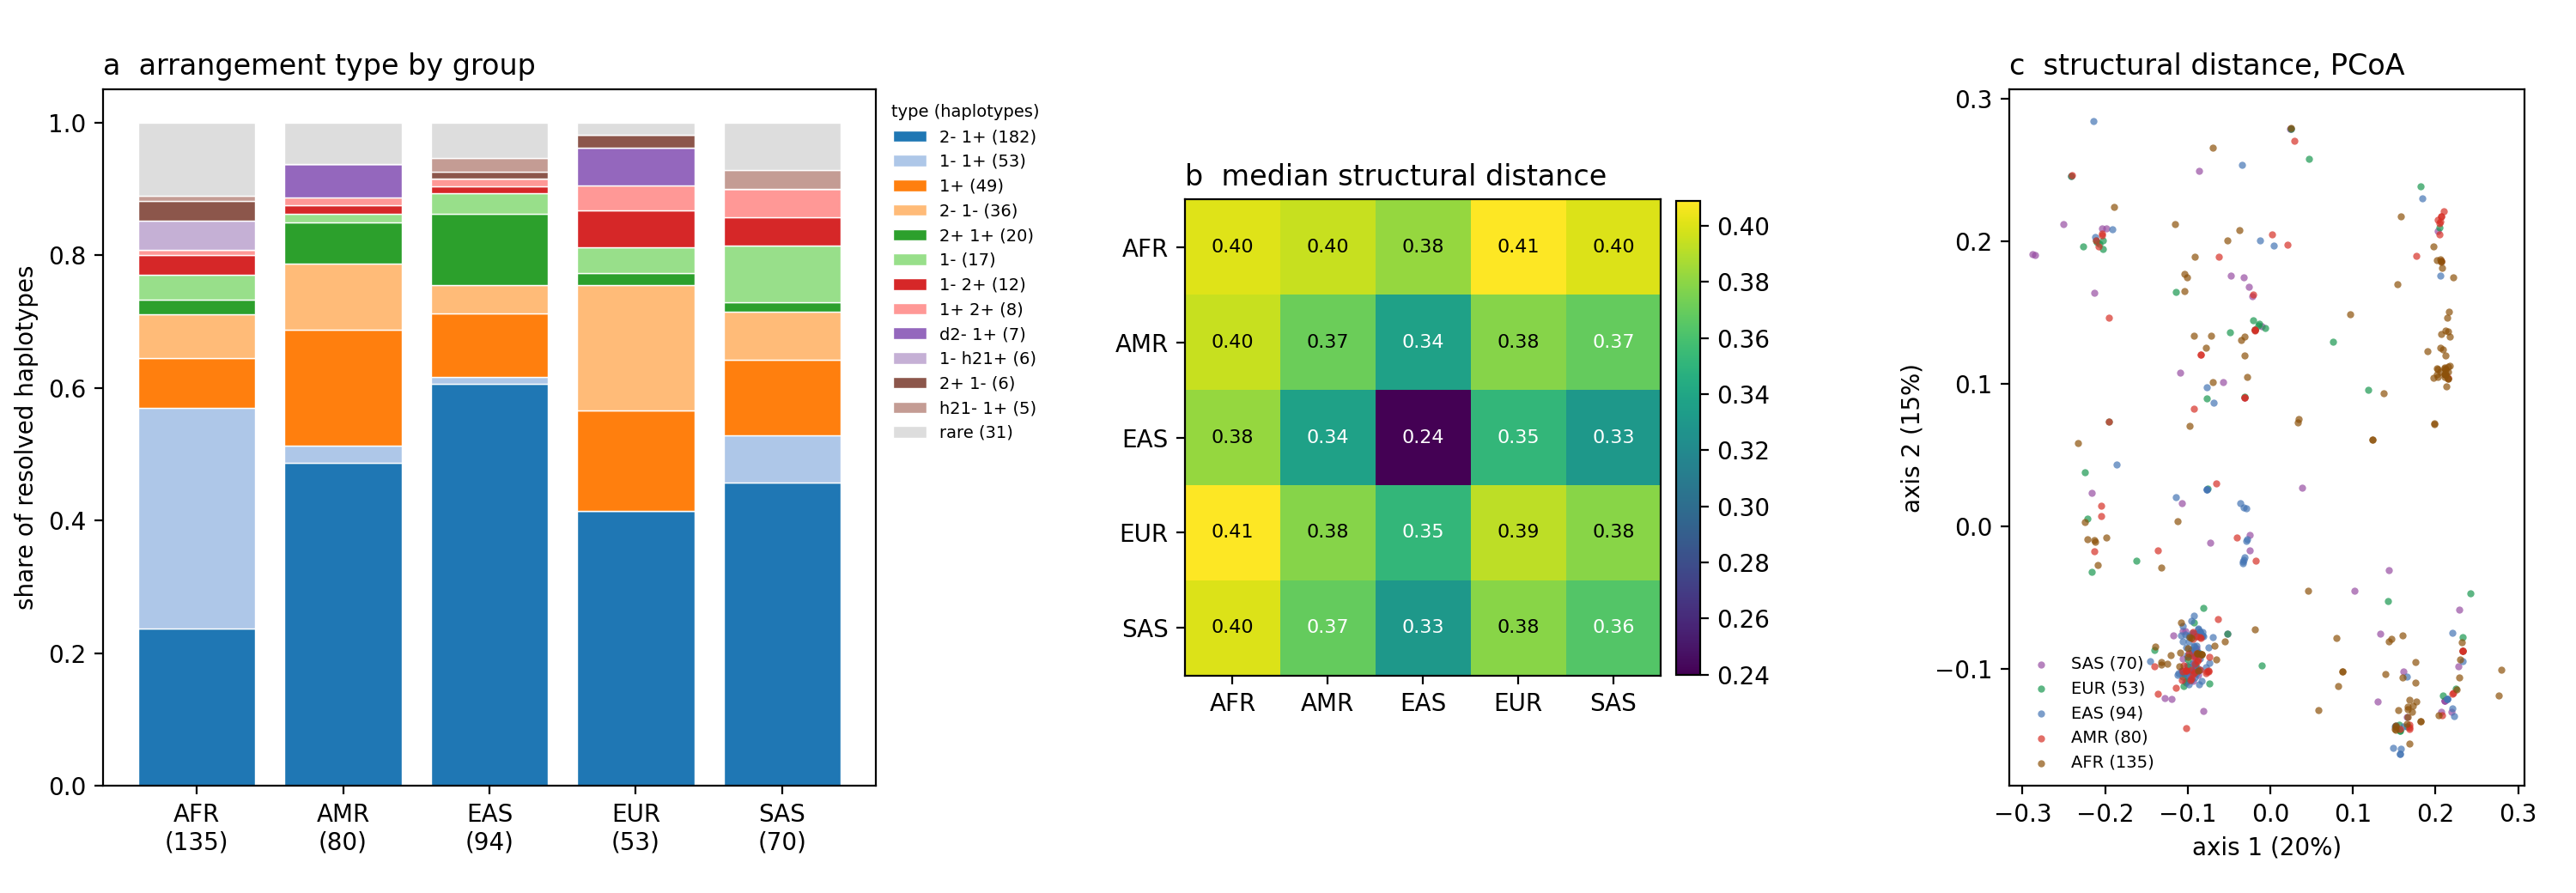
\includegraphics[width=\linewidth]{../figures/ancestry_structure.png}
\caption{Large-scale structure of the \anHaps{} resolved haplotypes by continental group. (a) Share of each
arrangement type (types on fewer than five haplotypes pooled as ``rare''; counts in the legend are over these
\anHaps{} haplotypes). (b) Median PANGEA structural distance within (diagonal) and between groups. (c) Principal
coordinates of the structural distance, one dot per haplotype, colored by group. Drawn by
\texttt{09\_ancestry\_structure.py}.}
\label{fig:ancestry}
\end{figure}

\section{Great-ape outgroups: one SMN copy per ape haplotype, and a proposed order of events (Fig.~\ref{fig:evo}, Table~\ref{tab:apes})}\label{sec:history}
\textbf{Question.} At the sites that set SMN1 lineage A, lineage B and SMN2 apart, which bases are ancestral, and
what order of events do they suggest? An outgroup is needed. Step 03 (\texttt{03\_outgroup\_alignment.sh}) adds the SMN gene body of chimpanzee, bonobo,
gorilla and orangutan (NCBI, the T2T primary assemblies of Table~\ref{tab:apes}) to the copy alignment as four more
rows, keeping its \nAlnCols{} columns (MAFFT \texttt{--add --keeplength}, which drops ape bases that would need new
columns);
\texttt{13b\_evolution\_sites.py} takes the gene-body columns where SMN1 (A and B together) and SMN2 are each at least
90\% fixed for different bases (\evS{} sites, ``paralog sites'') and those where A and B are (\evAB{} sites, ``A/B sites''),
and calls a base ancestral when at least three of the four apes carry it.

\textbf{How many SMN copies do the apes carry?} \texttt{14\_ape\_copies.py} and \texttt{15\_ape\_copies\_hap2.py}
search 5~Mb of each primary haplotype and 8~Mb (18~Mb for gorilla, whose chromosome is 7.7~Mb shorter) of each ape's
second haplotype for dense runs of SMN gene-body 25-mers. Each of the \apeHaps{} haplotypes holds exactly one copy
(\apeCopies{} copies), and a search at a lower density finds nothing outside these copies (on the second orangutan haplotype it returns \apeRelaxExtra{} further hit, inside that copy's own span; Table~\ref{tab:apes}). Across each whole genome, NCBI Gene lists
\apeGeneFull{} full-length SMN genes, one per ape at that locus, and \apeGeneShort{} other SMN-like records of
\apeShortMin--\apeShortMax{} bp elsewhere, which this study did not examine. Every ape copy carries SMN1's base at
c.840 (C) and c.*239 (G). Rochette et al.\ (abstract only)~\cite{rochette2001} reported 2--7 SMN copies per diploid
chimpanzee genome by quantitative PCR, and no SMN2 exon~7--8 bases in non-human primates. The one-copy finding in these
four individuals does not fit an SMN duplication that predates the human--chimpanzee split; whether the duplication is
human-specific or ape copy number varies between individuals is left open.

\textbf{Do the apes carry the large repeats? (Figs.~\ref{fig:apeself} and~\ref{fig:apehum}).} \texttt{35\_ape\_structure.py}
takes a 3-Mb stretch centered on each ape haplotype's SMN copy and plots it against itself with PANGEA's shimmer matcher
($w=\dpW$, $k=\dpK$, $r=\dpR$, the settings of the human dot plots), and against one human window, HG01099 mat
(Fig.~\ref{fig:locus}a), whose arm elements are known. None of the ape stretches shows a long off-diagonal line: they have
\apFarLo--\apFarHi{} dots per Mb more than 50~kb off the diagonal, the human window \apFarHum{} per Mb, and the ape dots off the diagonal
form short columns, as interspersed repeats do (Fig.~\ref{fig:apeself}). Against the human window (Fig.~\ref{fig:apehum}),
chimpanzee, bonobo and gorilla each place both human core arms on one ape stretch: \apShareLo--\apShareHi\% of each arm's
matches fall in the same \apWin-kb ape stretch, in the same order from the human axis (Spearman $\rho>0.9$ on each arm), so
the human plot folds into a V at the axis; Xi and Xd fold onto the same ape stretch again. In orangutan the matches are
sparse and at most \apOruShare\% fall in one stretch. S matches chimpanzee and bonobo at \apSPanLo--\apSPanHi{} times the
rate of the human window's unique flank, and gorilla and orangutan at no more than \apSOtherHi{} times it
(\path{results/sv/ape_fold.tsv}). One copy of the human core per ape haplotype, with both human arms on it, fits a
palindrome that formed in the human lineage after the split from these apes; the ape stretches are one assembly per
species and one human haplotype is the reference, and the absence of S in gorilla and orangutan is within 1.5~Mb of
the copy only.

\begin{figure}[htbp]\centering
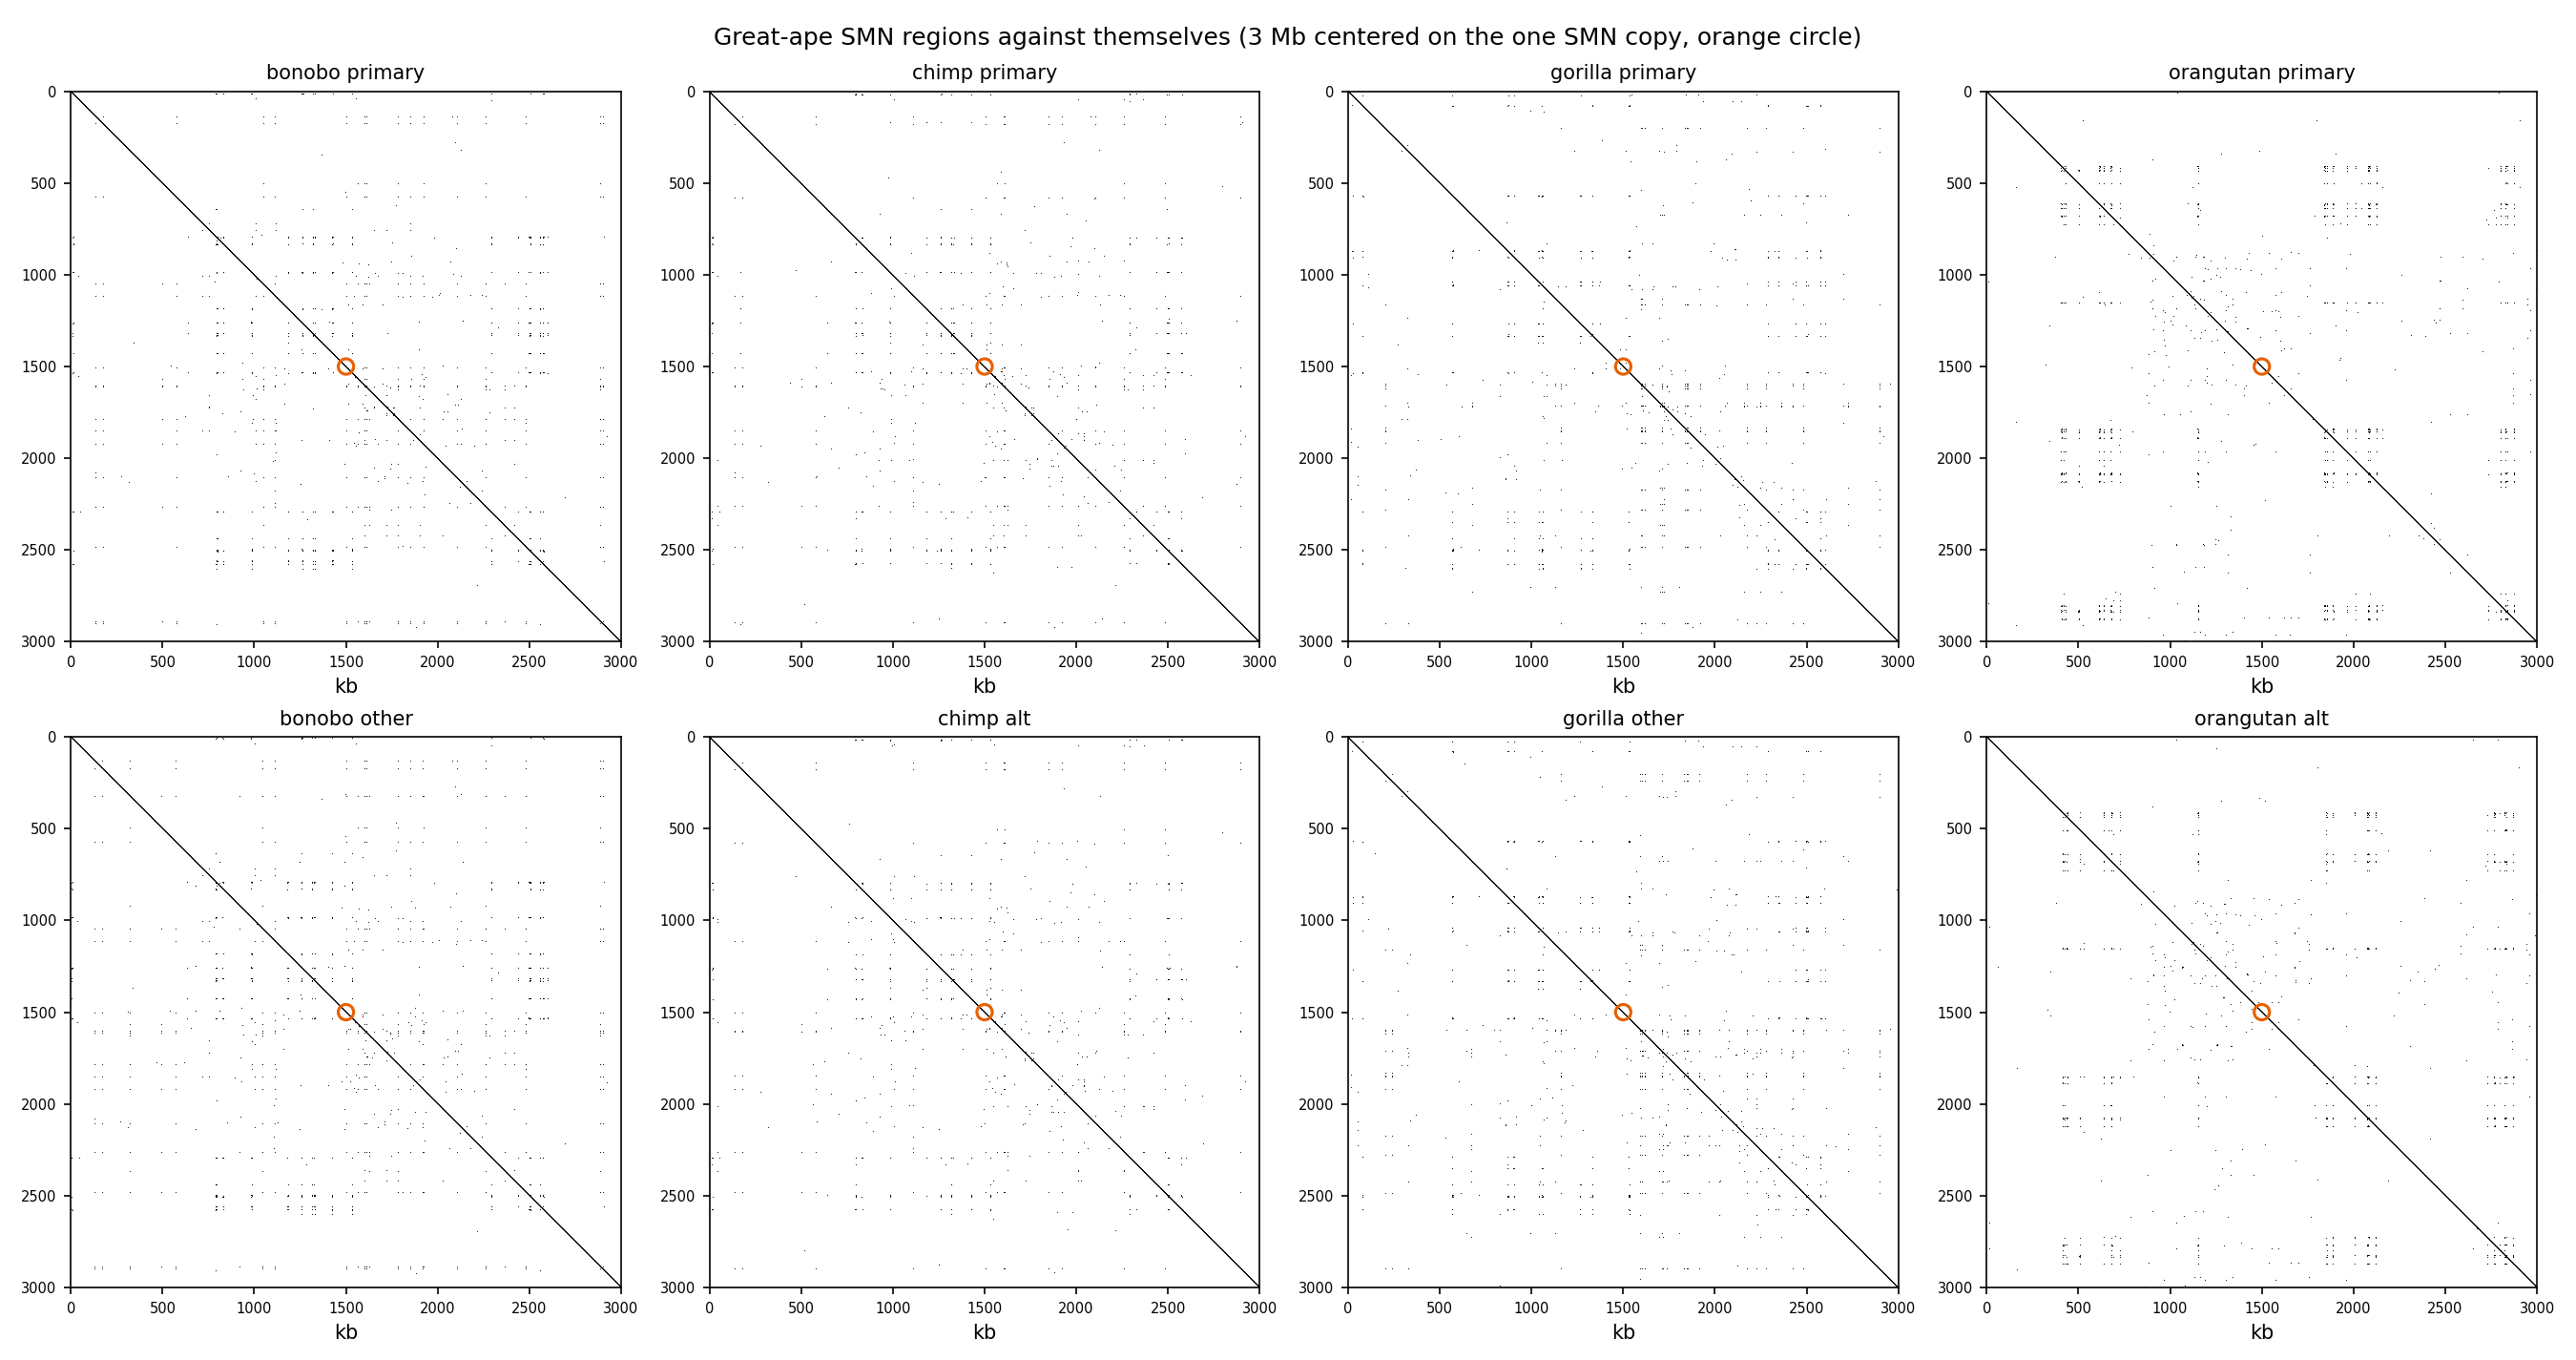
\includegraphics[width=\linewidth]{../figures/ape_self_dotplots.png}
\caption{Each great-ape haplotype's SMN region against itself: 3~Mb centered on its one SMN copy (orange circle), shimmer
matches as dots ($w=\dpW$, $k=\dpK$, $r=\dpR$). Only the main diagonal and short columns of interspersed repeats appear; no
long inverted or direct repeat. ``Other'' and ``alt'' are each ape's second haplotype assembly.}\label{fig:apeself}
\end{figure}

\begin{figure}[htbp]\centering
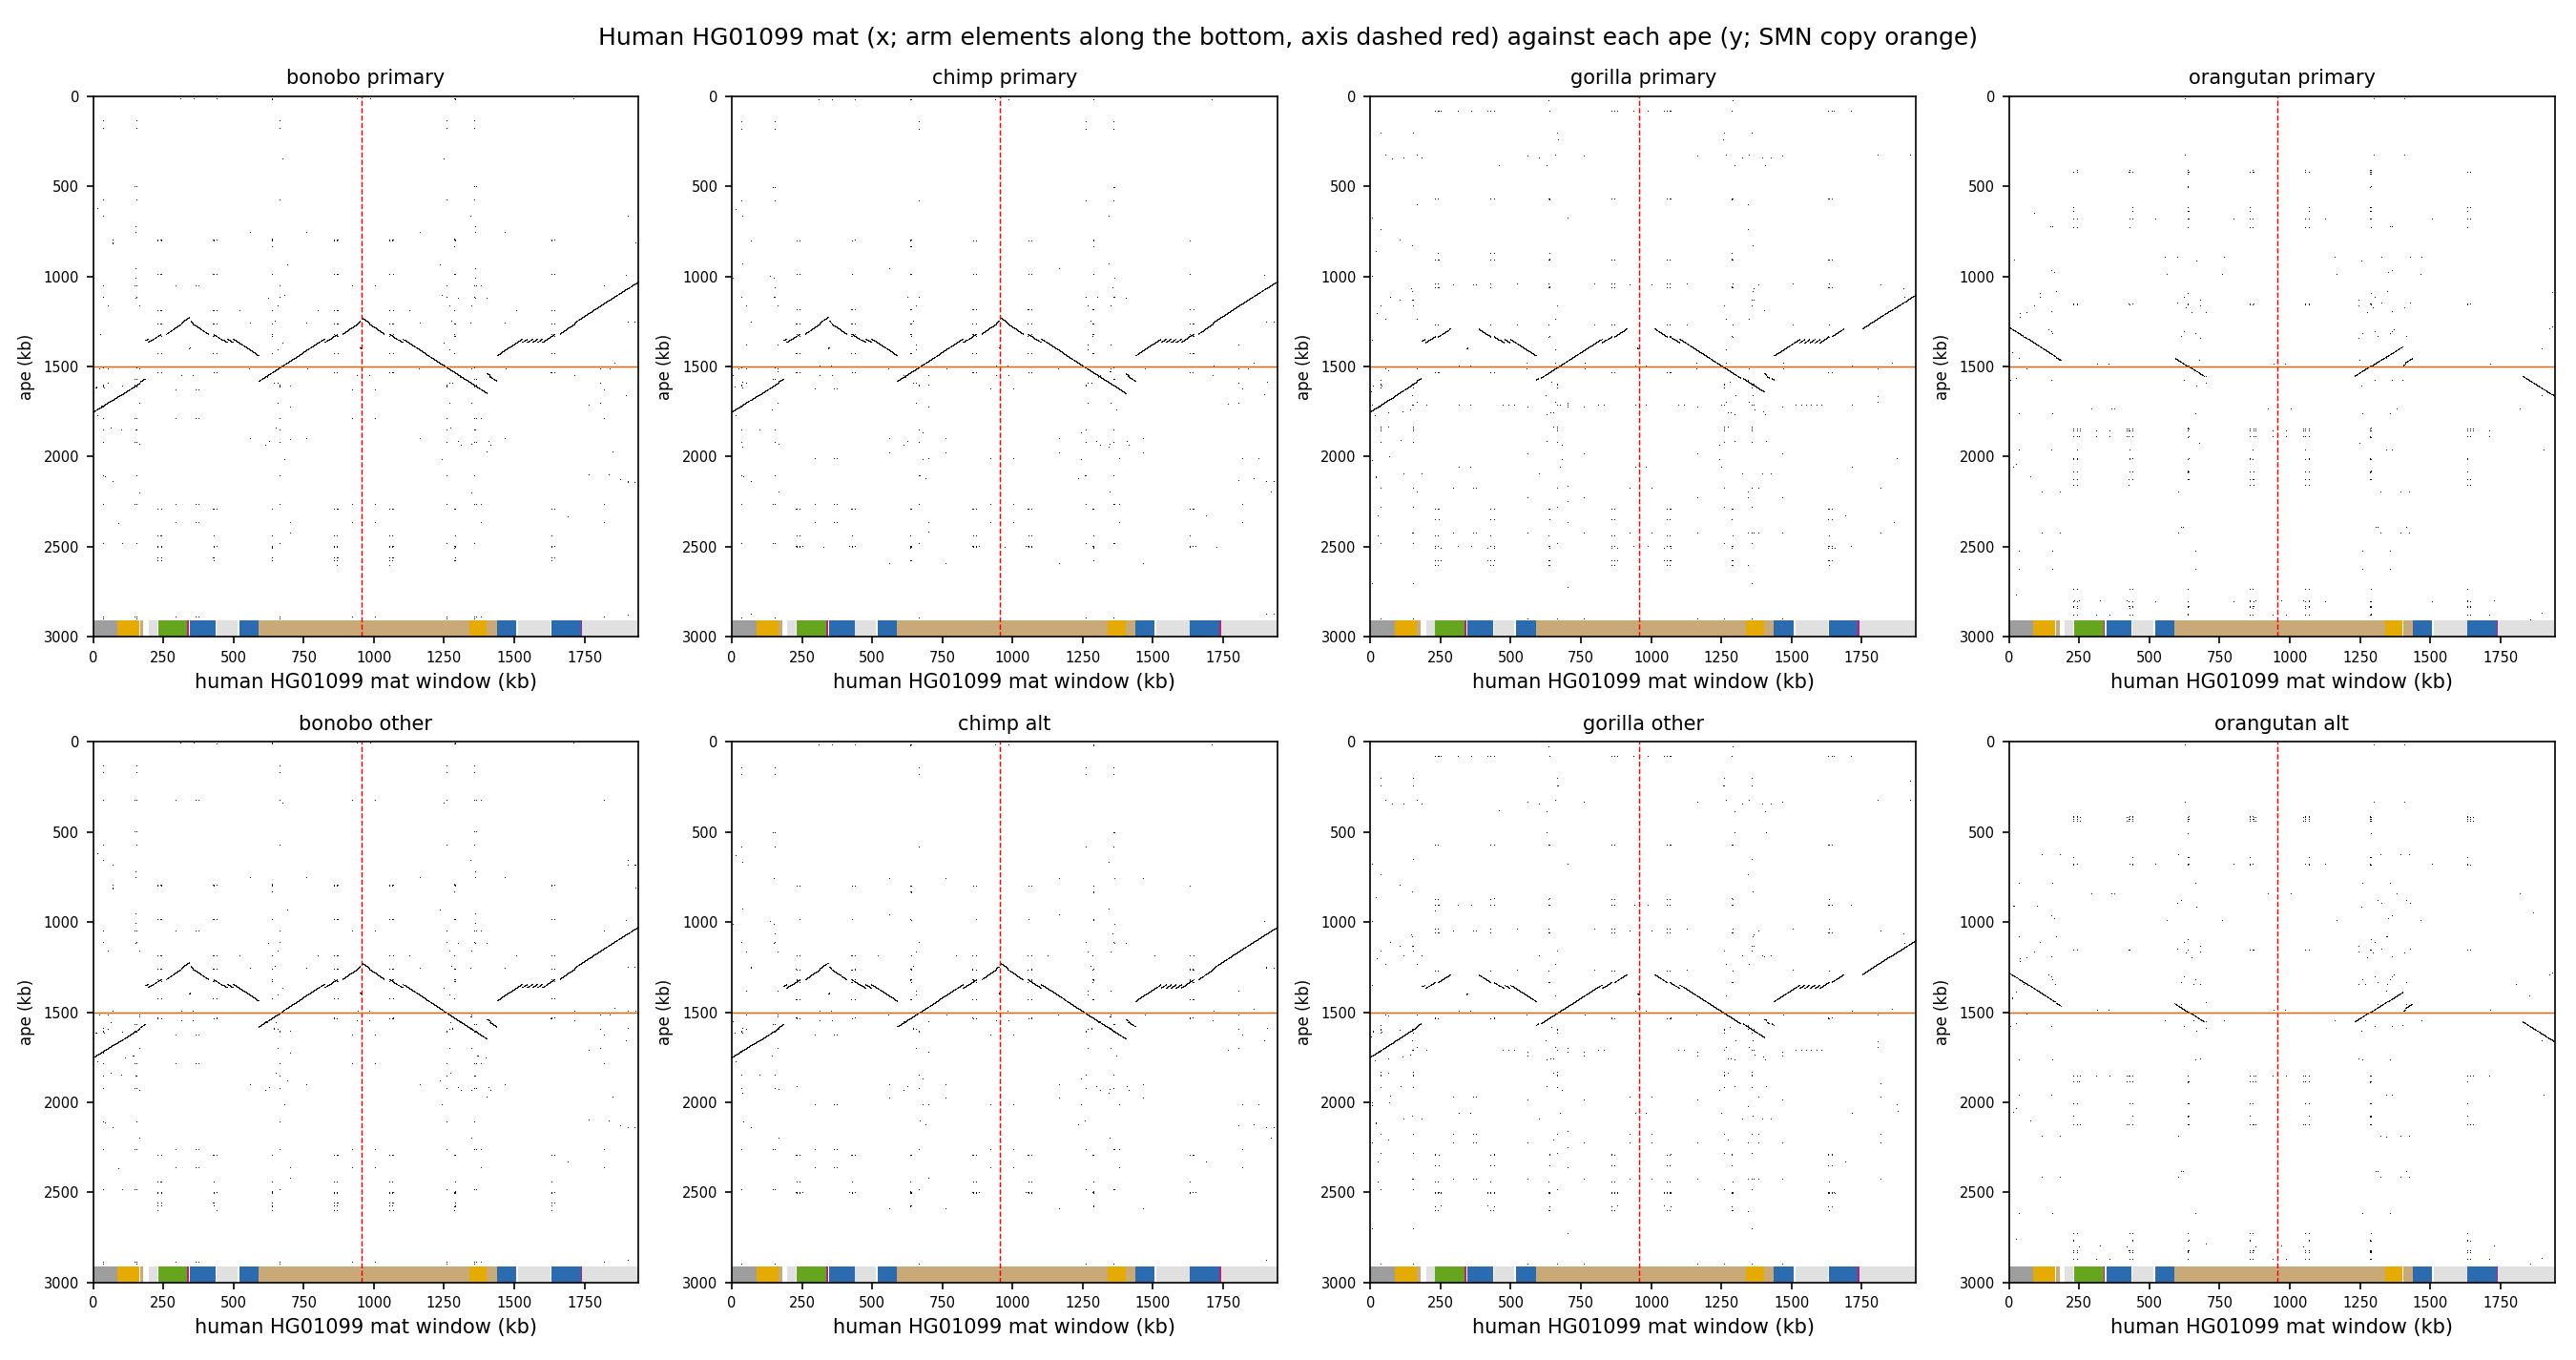
\includegraphics[width=\linewidth]{../figures/ape_vs_human.png}
\caption{The human window HG01099 mat (x; its arm elements along the bottom, colors as in Fig.~\ref{fig:palindrome};
axis of the \RU{A}+ \RU{A}$-$ pair dashed red) against each ape stretch (y; the ape SMN copy, orange line). In chimpanzee, bonobo and
gorilla both human arms run onto the same ape stretch, folding into a V at the human axis; in orangutan only short pieces
match.}\label{fig:apehum}
\end{figure}

\begin{table}[htbp]\small\centering
\caption{The SMN copy found in each great-ape haplotype searched: assembly sequence, start, strand, the bases at
c.840 and c.*239, and the base counts at the \evS{} paralog sites (SMN1/SMN2) and the \evAB{} A/B sites (A/B), each copy
aligned pair-wise to GRCh38 SMN1. Pair-wise counts can differ from the counts in the text, which use each ape's base read from its raw sequence (step~13c; see below); those read-checked counts are the last two columns, for the primary assemblies (unresolved sites counted in neither). ``Second'' is the species' other haplotype assembly. Each haplotype holds one whole SMN copy. The lower-density search finds nothing outside these copies; on the second orangutan haplotype it returns \apeRelaxExtra{} further hit, over \apeOrangPartCov{} of the gene body, which lies inside that copy's own span and on the opposite strand, and is not a second copy. From \texttt{results/sv/ape\_copies.tsv} and \texttt{results/sv/ape\_copies\_hap2.tsv}.}\label{tab:apes}
\footnotesize\setlength{\tabcolsep}{4pt}\begin{tabular}{@{}lllrlccrrrr@{}}\toprule
Ape & Haplotype & Sequence & Start & Strand & c.840 & c.*239 & paralog & A/B & paralog, read & A/B, read\\\midrule
\tabApes
\bottomrule\end{tabular}
\end{table}

\textbf{What the sites say.}
\begin{itemize}
\item \textbf{SMN1 against SMN2.} All \evS{} paralog sites lie in chr5:\evSfrom--\evSto{} (\evSspanKb{} kb, intron~6 to
exon~8). They are \bzMatch{} of the \bzPsvN{} paralogous sequence variants (PSVs) in Fig.~4 of Berzal-Serrano et al.~\cite{berzal2026}: \bzExact{} carry the same c.\ name there, and \bzOff{} in intron~6 sit \bzOffBp{} bases from theirs, with the same spacing and bases. Their PSVs \bzUnmatched{} are not among our paralog sites. The apes carry SMN1's base at \evSancOne{} (c.840 and c.*239 among them, so SMN2's bases there are new) and
SMN2's at \evSancTwo{} (unresolved \evSunres). A and B both carry SMN1's base at every paralog site, and share the newer
SMN1 base at \evSsharedAB: in this stretch A groups with B.
\item \textbf{A against B.} The \evAB{} A/B sites lie in chr5:\evABfrom--\evABto, between exon~1 (5$'$ untranslated part) and intron~2, upstream of that
stretch. The apes carry B's base at \evABancB{} and A's at \evABancA{} (unresolved \evABunres). Per ape, A's base at
\evABAChimp{} (chimpanzee), \evABABonobo{} (bonobo), \evABAGorilla{} (gorilla) and \evABAOrang{} (orangutan) sites. These ape bases are read from each ape's raw primary-assembly sequence, not from the multiple alignment: the 101-bp GRCh38 context of each site is aligned locally to the ape's region and the read kept when it covers the site at identity $\geq$0.85 with no gap within 3 bases (step~13c; \rdAcc{} of \rdN{} ape--site reads kept; a read not kept leaves the alignment's base only where the two agree). The kept reads differ from the multiple alignment in \rdMsaDiffN{} cases, \rdMsaDiff; the alignment had placed those orangutan bases wrongly. The weakest kept read is orangutan at chr5:\rdWeakSite: its best local match scores \rdWeakScore{} against \rdWeakSecond{} for the next best (\rdWeakOthLo--\rdWeakOthHi{} for the other three apes there). Set aside, the site would still carry B's base in chimpanzee, bonobo and gorilla; a second assembly per species would settle it. At \rdUnresSite, the last base of a run of 14 T before 5 G in GRCh38, no ape aligns cleanly across the site, so it is unresolved in all four (the alignment had given G, or a gap in orangutan). Pair-wise typing (Table~\ref{tab:apes}) differs from the read sequence in \apeDiffN{} site--ape cases (\apeDiffSites); the primary orangutan copy's pair-wise match is the weakest (21-mer share \apeOrangKmer, against \apeOtherKmerLo--\apeOtherKmerHi{} for the other apes).
\item \textbf{A with SMN2 upstream.} SMN2 carries A's base at \evABtwoEqA{} of the \evAB{} A/B sites. At \evABtwoEqAanc{}
of them A's base is the ape base, which groups nothing; at the other \evABsharedATwo, where B keeps the ape base, A and
SMN2 share the newer base. Upstream, A groups with SMN2, as the maximum-likelihood tree does over the whole gene body.
\end{itemize}

\textbf{A proposed order (a hypothesis, Fig.~\ref{fig:evo}).} (1) The human and ape lineages split, with one SMN copy
in the ancestor as far as these assemblies show; (2) the single ape copy is a mix at the paralog sites (SMN2's base at
\evTwoBaseChimp, \evTwoBaseBonobo, \evTwoBaseGorilla{} and \evTwoBaseOrang{} of them in chimpanzee, bonobo, gorilla
and orangutan); (3) the human copies divide into lineage B's side and a side holding A and SMN2, which share newer bases
upstream; (4) SMN2 gains its defining bases in the \evSspanKb-kb stretch, where A and B keep or share SMN1 bases; (5)
conversion and unequal crossing-over go on, giving the hybrids. The evidence conflicts by region: \evSsharedAB{} newer
bases group A with B in the intron~6--exon~8 stretch, and \evABsharedATwo{} group A with SMN2 upstream. Gene conversion
between copies, which Suzuki et al.~\cite{suzuki2026} report as putatively biased and one-way around
SMN, would give such a regional mix under other orders too. The evidence rests on \evS{} and \evAB{} sites and one copy
per ape haplotype; the maximum-likelihood tree adds the cautions of Section~\ref{m:hist}.

% figure fig:evo is in the main text



\section{The finer bundle scale: the same comparisons on a finer decomposition}\label{sec:fine}
Beside the study's bundle decomposition (step 00), a finer one, with more and shorter bundles, is run as a check (Table~\ref{tab:decomp}). Its repeat-unit families are written \RUf{A}, \RUf{B}, \dots; their letters are assigned separately from the study's \RU{A}, \RU{B}, \dots\ and do not correspond to them. The coarse
decomposition captures the large structure with fewer, longer bundles; the finer one keeps more detail. Both are run on
the same \wfN{} windows, and the structural distances they give have rank correlation \tsStructRho{} over all pairs of
windows. The main text uses the coarse one. This section reports what the finer one gives: the association tests,
recomputed on its distance (steps 01b and 28i), and the bands, arm forms, repeat-unit families and copy positions on it (step 37,
\path{results/sv/fine/}). Its set of
pair haplotypes (\fafTOneAll{} with a T1 and \fafTZeroAll{} with a T0 arm) differs slightly from the coarse one, so its counts are of its own set.

\begin{table}[htbp]\small\centering
\caption{The two bundle decompositions: every setting of \texttt{pangea cohort bundle decomp} (given on the command
line, or PANGEA's default where marked), and the result. Both are run on all windows together; \texttt{repeat-units}
is run on each at its default settings and \texttt{dist} with \texttt{--top-n \setTopN}. From
\texttt{results/sv/decomp\_params.tsv} (step 28i), the commands read from each BED file's header and the defaults from
\texttt{decomp --help}.}\label{tab:decomp}
\begin{tabular}{@{}lrr@{}}\toprule
Setting & Coarse (main text) & Finer (this section)\\\midrule
\tabDecomp
\bottomrule\end{tabular}
\end{table}

\paragraph{The association between structure and sequence (Table~\ref{tab:twoscales}).} With the same haplotypes, the same
sequence distances and the same shuffles, the Mantel correlation is a little higher on the finer decomposition in
\tsHigherFine{} of the \tsTests{} Mantel tests, the cophenetic correlation too (\tsCophC{} against \tsCophF), and every Mantel test has $p=$\,\mantelP{} at both scales. The difference is largest
within C0 arms (\tsCZeroC{} against \tsCZeroF) and absent within T1 arms (\tsTOneC{} against \tsTOneF). Finer
bundles may hold more of the link to the bases, but how much depends on the arm type: this is an observation, not a
rule. The two correlations of a test come from the same haplotypes, and no test of their difference was made.

\begin{table}[htbp]\small\centering
\caption{Mantel correlation (Spearman) between structural and SMN sequence distance at the two bundle scales, and the
cophenetic correlation of the structure tree (UPGMA) with the gene-body maximum-likelihood tree (Section~\ref{sec:cophen}). Arm-type rows use the SMN1 copies of haplotypes with that arm type, so the
type itself cannot make the correlation. Every Mantel $p\le$\,\mantelP{} (\nPerm{} shuffles, one seed per test shared
by both scales). From \texttt{results/sv/two\_scales.tsv} (step 28i).}\label{tab:twoscales}
\begin{tabular}{@{}lrrr@{}}\toprule
Test & Haplotypes & Coarse & Finer\\\midrule
\tabTwoScales
\bottomrule\end{tabular}
\end{table}

\paragraph{Bands (Table~\ref{tab:twoscalebands}).} With the same structure cut (\setK{} clusters) and the same
sequence clusters, the finer decomposition gives four bands. Three are the coarse bands again: the B1\,+\,B2 band
(all \fbABinCoarse{} of its \fbABn{} haplotypes are in the coarse one), the S1-2 band (\fbTwoinCoarse{} of its
\fbTwon{}, and all of the coarse one's) and the bulk (\fbBulkinCoarse{} of its \fbBulkn). The fourth is an S1-3 band of
\fbThreen{} haplotypes (\fbThreeexp{} expected, $p=\fbThreep$), mostly ``2-~1+'' and ``1+'', each with one forward
SMN1 copy of haplogroup S1-3. On the coarse decomposition these haplotypes fall in the bulk's structure cluster
(\fbThreeToBulk) and the B1\,+\,B2 band's (\fbThreeToAB), and form no band.

\begin{table}[htbp]\small\centering
\caption{The bands at the two bundle scales (sequence side from the supported maximum-likelihood clades in both).
$n$, haplotypes; exp., expected by chance; $p$, Bonferroni-corrected hypergeometric. Coarse: \texttt{results/sv/ml\_vs\_upgma\_bands.tsv};
finer: \texttt{results/sv/fine/ml\_vs\_upgma\_bands.tsv}.}\label{tab:twoscalebands}
\begin{tabular}{@{}lrrrrrr@{}}\toprule
& \multicolumn{3}{c}{Coarse} & \multicolumn{3}{c}{Finer}\\\cmidrule(lr){2-4}\cmidrule(lr){5-7}
Band & $n$ & exp. & $p$ & $n$ & exp. & $p$\\\midrule
Bulk & \cbBulkn & \cbBulkexp & $\cbBulkp$ & \fbBulkn & \fbBulkexp & $\fbBulkp$\\
S1-2 band & \cbTwon & \cbTwoexp & $\cbTwop$ & \fbTwon & \fbTwoexp & $\fbTwop$\\
S1-3 band & -- & -- & -- & \fbThreen & \fbThreeexp & $\fbThreep$\\
B1\,+\,B2 band & \cbABn & \cbABexp & $\cbABp$ & \fbABn & \fbABexp & $\fbABp$\\\bottomrule
\end{tabular}
\end{table}

\paragraph{The structure clusters against arm form.} On the finer decomposition the S1-3 and B1\,+\,B2 bands shared one
structure cluster (\fafMixClu{} haplotypes), and the clusters split by the telSMN arm type rather than the cenSMN one:
all \fafMixPair{} haplotypes with the pair in that cluster had a T1 arm (\fafMixCOne{} C1|T1, \fafMixCZero{} C0|T1),
and none of the \fafBulkPair{} in the bulk's cluster (\fafBulkClu{} haplotypes; Fisher $p=$\,\fafP). The S1-3 band held
\fafThreePair{} haplotypes with the pair, all C1|T1, and \fafThreeNoPair{} without it; the B1\,+\,B2 band's
\fafABCZTOne{} were all C0|T1. So the cenSMN arm separates the two large clusters on the coarse decomposition, and the
telSMN arm on the finer one; which arm the structural distance weighs most depends on the bundle scale.

\paragraph{Family~\RUf{G} and the S1-3 band.} On the finer decomposition a repeat-unit family~\RUf{G}, a unit of median \sGkb{} kb,
was on all \sBandG{} S1-3 band haplotypes and on \sCenG{} of the \sCen{} in the bulk; restricted to ``2-~1+''
haplotypes, \sBandTwoOneG{} of \sBandTwoOneN{} against \sCenTwoOneG{} of \sCenTwoOneN{}.
Family~\RUf{C} was on \sBandC{} of \sBand{} against \sCenC{} of \sCen, and family~\RUf{D} on \sBandD{} against \sCenD. Across the
\sHaps{} resolved haplotypes with an SMN1 copy, \sGandT{} of the \sTall{} carrying an S1-3 copy had an \RUf{G} unit, but so
did \sGnotT{} others, so \RUf{G} was not specific to S1-3. Among \RUf{G} carriers, the S1-3 haplotypes (\sGThreeC{} of \sGThreen{}
with \RUf{C}) and the S1-2 haplotypes (\sGTwoC{} of \sGTwon{}) shared the \RUf{C} units and mostly lacked \RUf{D}, while the
S1-8/S1-9/S1-6 haplotypes carried \RUf{D} (\sGEightD{} of \sGEightn) and rarely \RUf{C} (\sGEightC). In elements, \RUf{G} was Xi with S
(\ffeGcombo{} of its \ffeGocc{} occurrences on haplotypes with the pair), on \fafGTOne{} of the \fafTOneAll{}
haplotypes with a T1 arm and \fafGTZero{} of the \fafTZeroAll{} with T0: the T1 arm under another name. On the coarse decomposition the family that
marks the T1 arm is \RU{\afSigFam} (Section~\ref{sec:bands}).

\paragraph{Why the copy sits further out on C0 and T1 arms.} On the finer decomposition the stretch of the core between
bundles 40 and 16 holds the inner $\sim$20-kb array. It was a median \fcpArrCZero~kb on the \fcpNCZero{} C0 arms
against \fcpArrCOne~kb on the \fcpNCOne{} C1 arms (the arms on which both bundles were found), one unit more, while the rest of the axis-to-copy distance was the
same (\fcpRestCZero{} and \fcpRestCOne~kb): the C0 copy's extra \fcpDiffCopycen~kb was the stretch
(\fcpDiffArrcen~kb). On the telSMN arm, T1 against T0, the stretch was \fcpArrTOne{} against \fcpArrTZero~kb and the
rest \fcpRestTOne{} against \fcpRestTZero~kb. The stretch took few lengths, \fcpModes~kb, one array unit apart
(Spearman correlation of copy distance with the stretch \fcpRhocen{} on the cenSMN and \fcpRhotel{} on the telSMN
arm; \path{results/sv/fine/copy_position.json}).

\paragraph{Why the finer unit call split \RUf{A} into long and short.} On the finer decomposition PANGEA's \texttt{repeat-units} called an \RUf{A} unit long (\elUnitLong~kb or more, the same cut as in Section~\ref{sec:palindrome}) on some arms and short on others, and the two did not follow the arm elements. HG03816 pat and HG01099 mat (the top two windows of Fig.~\ref{fig:pgraph}) carry the same arm elements in the same order, yet with the finer bundles PANGEA called a short \RUf{A}+ unit with \RUf{B}$-$
beyond it in the first and one long \RUf{A}+ unit in the second. Only the tandem arrays differ: the outer array of the telSMN arm
has \grPatTel{} units of 18~kb in the first against \grMatTel{} in the second, and that of the cenSMN arm \grPatCen{}
against \grMatCen{} units of 20.5~kb.

Applying the chain score of step~2 of the algorithm (Section~\ref{sec:compared}) to these two windows shows that the call turned on how unequal the tandem arrays on the two arms are,
not on a difference in content. It is one case of the general rule given in Section~\ref{m:arms} and Fig.~\ref{fig:locus}:
an \RU{A} unit ends where the two arms, read outward from the axis, stop matching each other, earlier on some
haplotypes and later on others; the elements do not move
(Section~\ref{sec:palindrome}).


\section{How each figure and number is made}\label{sec:provenance}
Every figure is drawn, and every number of this document is written, by a numbered step of the pipeline
(\texttt{scripts/run\_all.sh} runs them in order). Fig.~\ref{fig:provenance} shows, step by step, which inputs each one
reads, which earlier steps' files it reads, which figures it draws and how many of the document's numbers read its
files. The reads and writes of the Python steps are not declared by hand: \texttt{scripts/trace\_io.py} runs each step
and records every project file it opens, through Python's audit hook (\texttt{results/sv/provenance\_io.tsv}); the four
shell steps, which run PANGEA, MAFFT and IQ-TREE, declare theirs in \texttt{41\_provenance.py}, which checks that the
files exist. Rerunning all Python steps under this trace reproduced every result table and figure byte for byte.
\texttt{40\_numbers.py} writes the \pvNumbers{} numbers as macros, each with the script line that computes it, the
files it reads and the checks that guard the sentence around it (\texttt{note/numbers.json}); the build stops if a
check fails. Table~\ref{tab:numsrc} lists, for each of the \pvFiles{} files the numbers read, the step that writes it,
how many numbers read it and where in the document it is used. A number that reads several files (\pvMulti{} of
them) is counted under each.

\begin{figure}[htbp]\centering
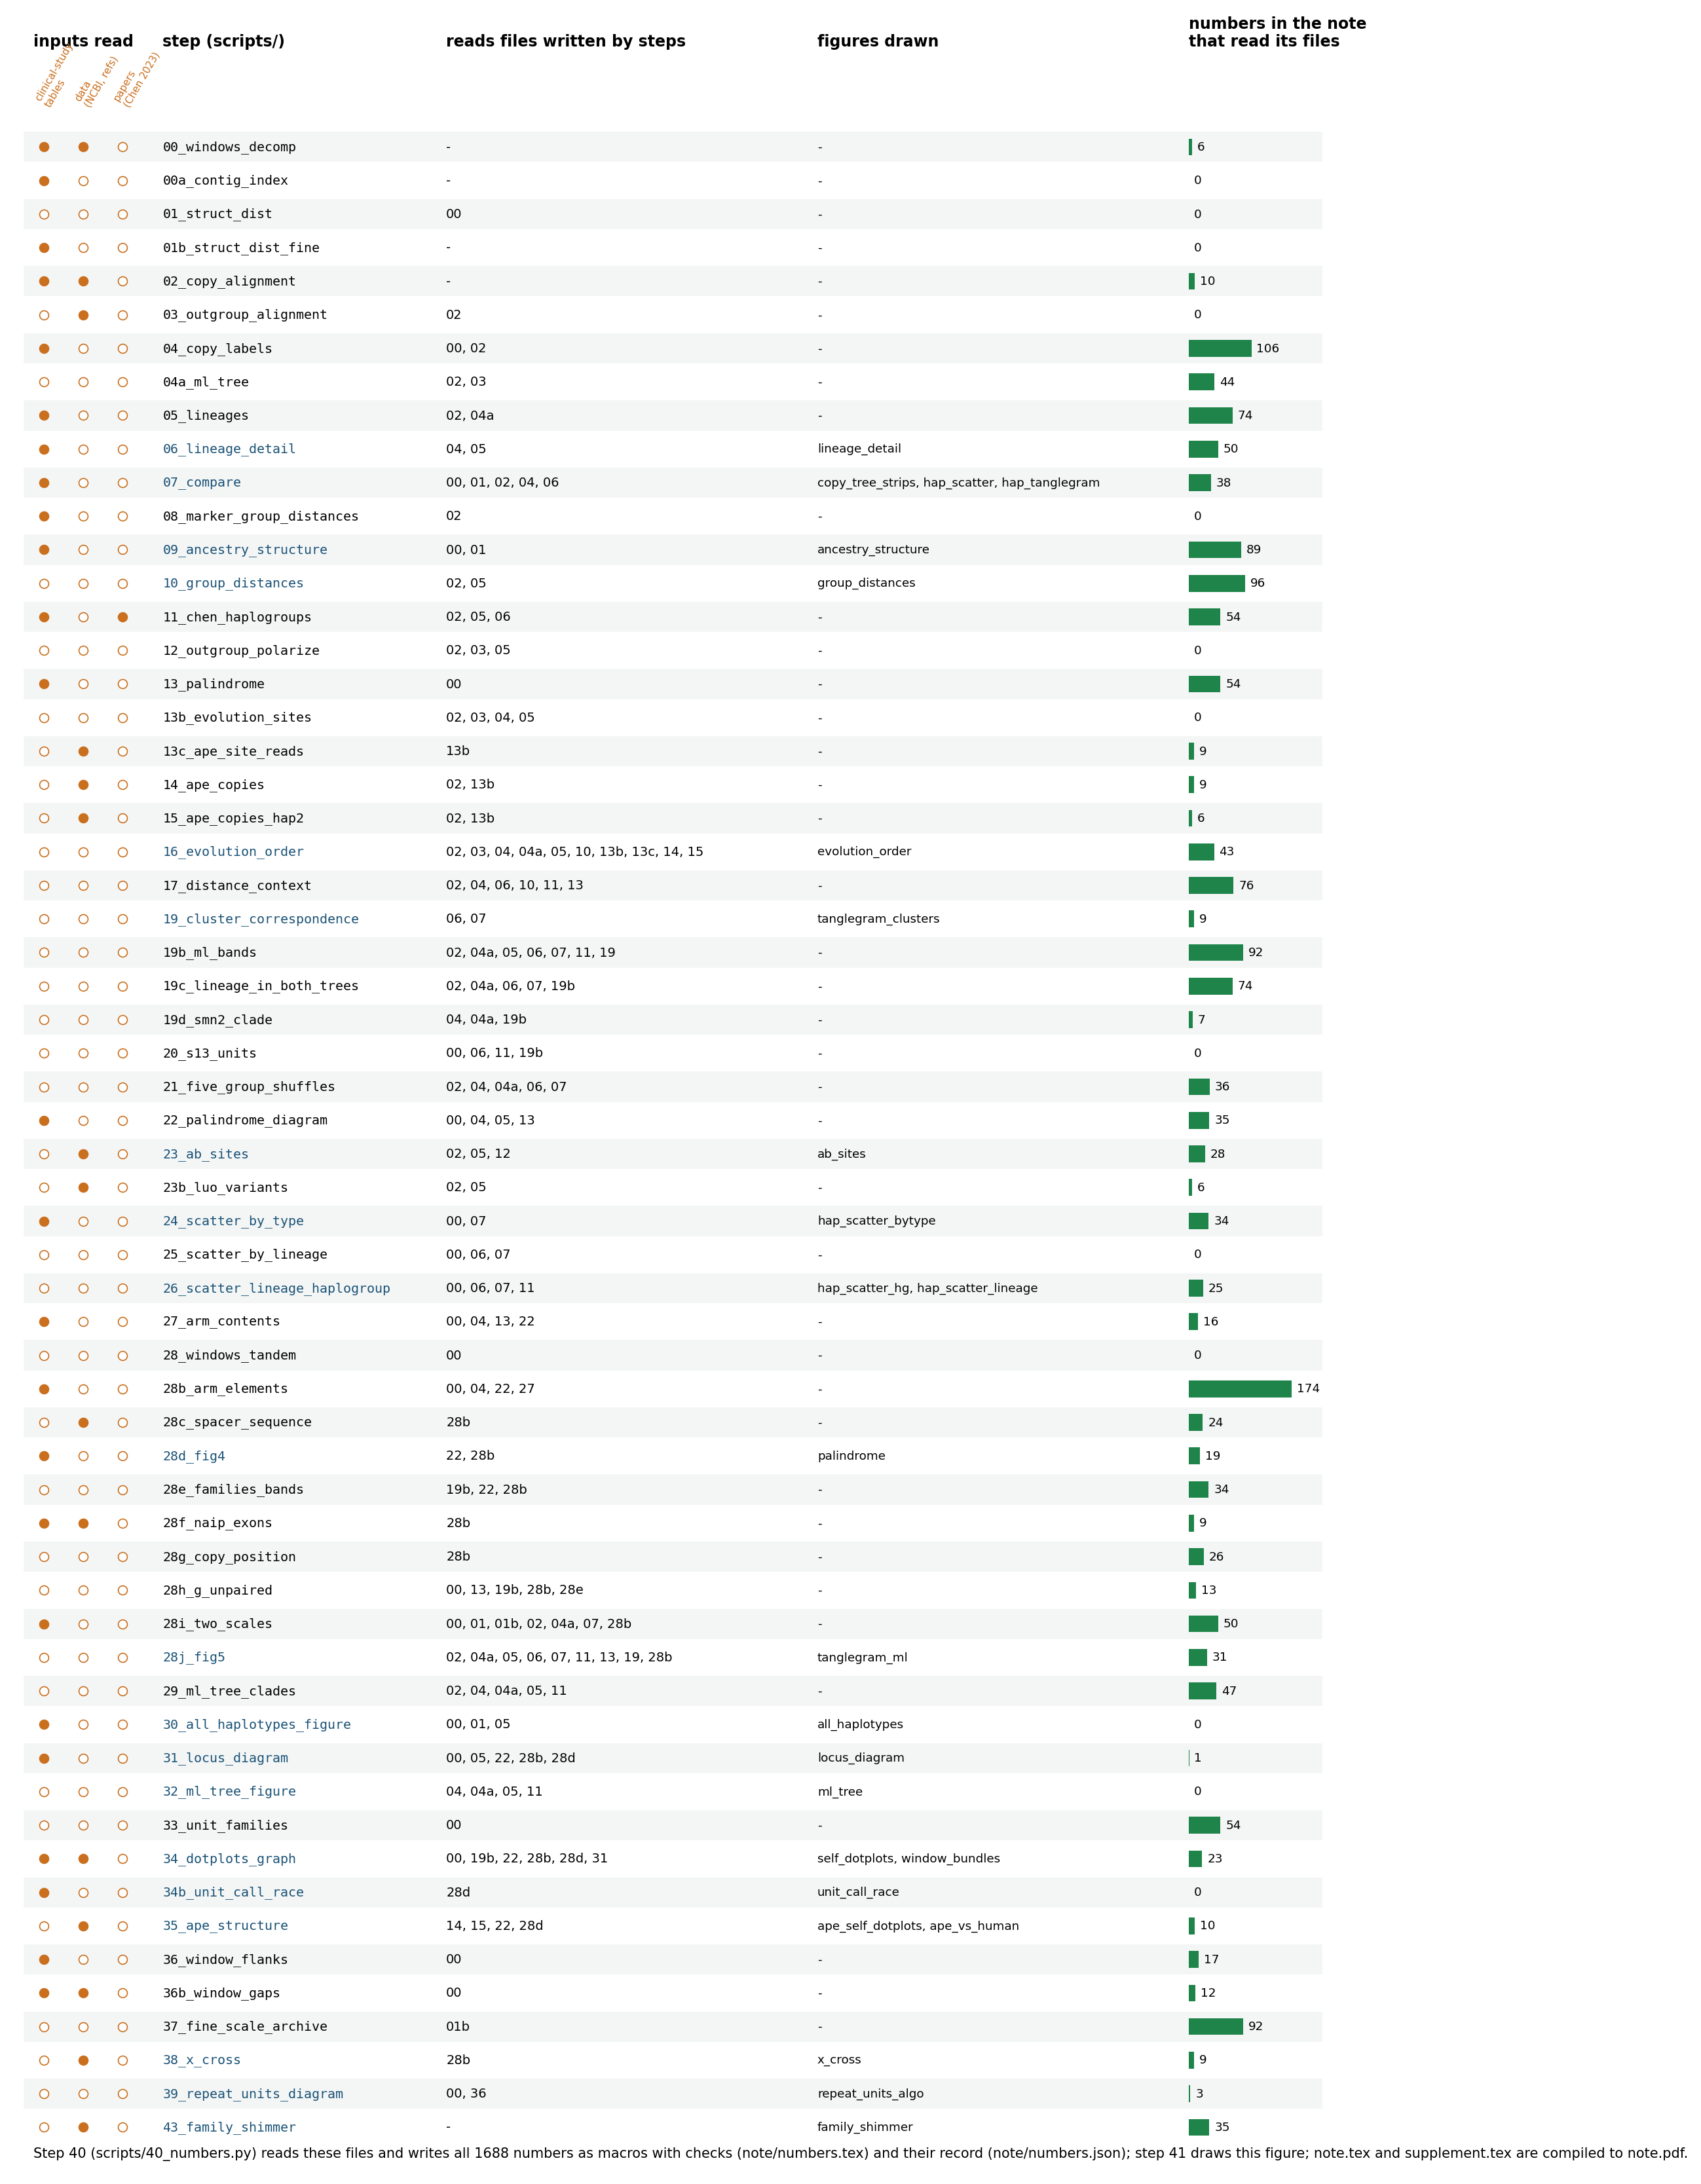
\includegraphics[width=\linewidth]{../figures/provenance.png}
\caption{The pipeline, one row per step in run order. Left, the inputs each step reads (orange dots: the clinical
study's tables, NCBI data and references, Chen et al.'s supplementary tables); then the earlier steps whose files it
reads; the figures it draws (step names in blue); and how many of the document's numbers read its files (green bars).
Python steps' reads and writes are traced at run time; shell steps' are declared. Drawn by
\texttt{41\_provenance.py} from \texttt{results/sv/provenance\_io.tsv} and \texttt{note/numbers.json}.}
\label{fig:provenance}
\end{figure}

{\footnotesize
\begin{longtable}{@{}>{\raggedright}p{5.6cm}>{\raggedright}p{1.4cm}r>{\raggedright}p{4.2cm}>{\raggedright\arraybackslash}p{2.2cm}@{}}
\caption{Where the numbers come from: each file the document's numbers read (in \texttt{results/sv/} unless a path is given), the step that writes it (``input'':
not written by this pipeline; ``setting'': a method setting read from a script), how many numbers read it, two of
them by macro name, and where the file is used (from \texttt{results/ledger.tsv}). Written by
\texttt{41\_provenance.py} from \texttt{note/numbers.json}.}\label{tab:numsrc}\\
\toprule
File & Step & Numbers & Example macros & Used in\\\midrule\endfirsthead
\toprule
File & Step & Numbers & Example macros & Used in\\\midrule\endhead
\tabNumSrc
\bottomrule
\end{longtable}}
